\documentclass[14pt,a4paper]{report}
\usepackage[utf8]{inputenc}
\usepackage[vietnamese=nohyphenation]{hyphsubst}
\usepackage[vietnamese]{babel}
\usepackage{titlesec, blindtext, color}
\usepackage[table,xcdraw]{xcolor}
\usepackage{multibib}
\newcites{web}{Website}

\title{THIẾT KẾ HỆ THỐNG AIOT PHÁT HIỆN VÀ CẢNH BÁO BẤT THƯỜNG CHO MÁY GIẶT DÂN DỤNG SỬ DỤNG AUTOENCODER KHÔNG GIÁM SÁT TRÊN THIẾT BỊ BIÊN}
\author{Quách Ngọc Quang}

\definecolor{gray75}{gray}{0.75}
\newcommand{\hsp}{\hspace{6pt}}
\usepackage{environ}
\NewEnviron{my_equation}{%
\begin{equation}
\scalebox{1.3}{$\BODY$}
\end{equation}
}
\titleformat{\chapter}[hang]{\small\bfseries}{\thechapter\hsp\textcolor{gray75}{|}\hsp}{0pt}{\Huge\bfseries}

\usepackage[left=3cm,right=2cm,top=2.5cm,bottom=3cm]{geometry}
\setlength{\parindent}{1cm}
\usepackage{indentfirst}   
\setlength{\parskip}{6pt}

%Section and Numbering Formatting
\setcounter{secnumdepth}{3}
\setcounter{tocdepth}{2}
\renewcommand\thesubsubsection{\Alph{subsubsection}}

\usepackage{sectsty}
\chapterfont{\centering}
\renewcommand{\baselinestretch}{1.3} %format distance between lines
\usepackage{xcolor}
\usepackage[unicode]{hyperref}
\hypersetup{
colorlinks = false,
linkbordercolor = {white}
}
\usepackage{xurl}
\Urlmuskip=0mu plus 1mu
\usepackage{graphicx}
\usepackage{lmodern}
\usepackage[font=large,labelfont=bf,labelsep=newline,justification=centering]{caption} % Tên ở trên, mô tả ở dưới (sau), căn giữa

% abbreviation
\usepackage{nomencl}
\makenomenclature
\renewcommand{\nomname}{Bảng ký hiệu và chữ viết tắt}
%% This code creates the groups
% -----------------------------------------
\usepackage{etoolbox}
\renewcommand\nomgroup[1]{%
  \item[\bfseries
  \ifstrequal{#1}{T}{Chữ viết tắt}{%
  \ifstrequal{#1}{K}{Ký hiệu}}%
]}
% ------

\usepackage{kantlipsum}
\usepackage{listings}
\usepackage{subcaption}
\usepackage{bm}
\usepackage[para]{footmisc}
\usepackage{amsfonts}
\usepackage{afterpage}
\usepackage{float}
\usepackage{tikz}
\usepackage{pdfpages}
\usepackage{xspace}
\usepackage{multirow}
% \usepackage{subfiles}

\usepackage{algorithm}
% \usepackage{algorithm2e} 
\usepackage{algorithmic}

\renewcommand{\listalgorithmname}{Danh sách thuật toán}
\renewcommand{\lstlistingname}{Đoạn mã}
\renewcommand{\lstlistlistingname}{Danh sách đoạn mã}
\renewcommand{\algorithmicrequire}{\textbf{Given:}}
\renewcommand{\algorithmicensure}{\textbf{Step }\textbf{Input :}}

\usepackage{physics}
\usepackage{amsmath}
\usepackage{amssymb}
\usepackage{amsthm}
\usepackage{tabularx, booktabs, makecell, caption}
\usepackage{siunitx}
\usepackage{adjustbox}

\usetikzlibrary{calc}
\usepackage{frontespizio}
% \usepackage[perpage]{footmisc}
\usepackage{perpage}
\MakePerPage{footnote}
\usepackage{longtable}
% \usepackage[backend=biber,style=ieee,sorting=none]{biblatex}
% \addbibresource{reference.bib}
% format titile chapter section ...
\titleformat{\chapter}[display]
{\large}
{
	\large\MakeUppercase{\chaptertitlename}~\thechapter}
{1pc}
{\titlerule\huge}

\titleformat*{\section}{\normalfont \Large}
\titleformat*{\subsection}{\normalfont \large}

\newtheorem{theorem}{Định lý}
\newtheorem{proposition}{Mệnh đề}
\newtheorem{assumption}{Giả thiết}
\newtheorem{lemma}{Bổ đề}
\newtheorem{remark}{Nhận xét}
\newtheorem{definition}{Định nghĩa}

\newenvironment{vietnamesealgorithm}[1][]
  {\begin{algorithm}[#1]
    \hrule height:.8pt depth:0pt
     \selectlanguage{vietnamese}%
     \floatname{algorithm}{Thuật toán}%
      \renewcommand{\algorithmicrequire}{\textbf{Given}}%
      \renewcommand{\algorithmicensure}{\textbf{Step}}
  }
  {\end{algorithm}}

\begin{document}

%doubleshot titlepage's border
\begin{tikzpicture}[overlay,remember picture]
    \draw [line width=0.8mm]
        ($ (current page.north west) + (2cm,-1.5cm) $)
        rectangle
        ($ (current page.south east) + (-1.5cm,1.5cm) $);
    \draw [line width=0.1mm]
        ($ (current page.north west) + (2.2cm,-1.7cm) $)
        rectangle
        ($ (current page.south east) + (-1.7cm,1.7cm) $);
\end{tikzpicture}

% ================= TRANG BÌA CHÍNH =================
\begin{center}
    {\fontsize{13}{1.3}\selectfont \textbf{ĐẠI HỌC QUỐC GIA HÀ NỘI\\TRƯỜNG ĐẠI HỌC CÔNG NGHỆ}\par}
                    
    \vspace{1.0cm}
            
    
\includegraphics[clip, scale=0.2]{uet.png}
    \vspace{0.5cm}
                                
    {\fontsize{14pt}{16pt}\selectfont \textbf{Quách Ngọc Quang}\par}
    \vspace{1.5cm}
                                
    % TIÊU ĐỀ 3 DÒNG: Đã thêm \par để đảm bảo khoảng cách dòng đều tuyệt đối
    {\fontsize{18pt}{22pt}\selectfont \textbf{THIẾT KẾ HỆ THỐNG AIOT PHÁT HIỆN VÀ CẢNH BÁO BẤT THƯỜNG CHO MÁY GIẶT DÂN DỤNG SỬ DỤNG AUTOENCODER KHÔNG GIÁM SÁT TRÊN THIẾT BỊ BIÊN}\par}
    
    \vspace{1.75cm}

    {\fontsize{13pt}{15pt}\selectfont \textbf{ĐỒ ÁN TỐT NGHIỆP ĐẠI HỌC HỆ CHÍNH QUY\\ \vspace{0.23cm} Ngành: Kỹ thuật Máy tính}\par}

    \vfill
    
    {\fontsize{12}{1.3}\selectfont \textbf{HÀ NỘI - 2026}\par}
\end{center}
\pagenumbering{gobble}

% ================= TRANG BÌA LÓT =================
\pagebreak
\begin{tikzpicture}[overlay,remember picture]
    \draw [line width=0.8mm]
        ($ (current page.north west) + (2cm,-1.5cm) $)
        rectangle
        ($ (current page.south east) + (-1.5cm,1.5cm) $);
    \draw [line width=0.1mm]
        ($ (current page.north west) + (2.2cm,-1.7cm) $)
        rectangle
        ($ (current page.south east) + (-1.7cm,1.7cm) $);
\end{tikzpicture}

\begin{center}
    {\fontsize{13}{1.3}\selectfont \textbf{ĐẠI HỌC QUỐC GIA HÀ NỘI\\TRƯỜNG ĐẠI HỌC CÔNG NGHỆ}\par}
                    
    \vspace{1.55cm}
                                
    {\fontsize{14pt}{16pt}\selectfont \textbf{Quách Ngọc Quang}\par}
    \vspace{1.5cm}
                                
    % TIÊU ĐỀ 3 DÒNG: Đã thêm \par để đảm bảo khoảng cách dòng đều tuyệt đối
    {\fontsize{18pt}{22pt}\selectfont \textbf{THIẾT KẾ HỆ THỐNG AIOT PHÁT HIỆN VÀ CẢNH BÁO BẤT THƯỜNG CHO MÁY GIẶT DÂN DỤNG SỬ DỤNG AUTOENCODER KHÔNG GIÁM SÁT TRÊN THIẾT BỊ BIÊN}\par}

    \vspace{2.5cm}

    {\fontsize{13pt}{15pt}\selectfont \textbf{ĐỒ ÁN TỐT NGHIỆP ĐẠI HỌC HỆ CHÍNH QUY\\ \vspace{0.23cm} Ngành: Kỹ thuật Máy tính}\par}
    
    \vspace{1.8cm}

    {\fontsize{13pt}{16pt}\selectfont
    \begin{tabular}{rl}
        \textbf{Cán bộ hướng dẫn:} & \textbf{TS. Nguyễn Kiêm Hùng} \\
        \textbf{Cán bộ đồng hướng dẫn:} & \textbf{TS. Mai Linh}
    \end{tabular}\par}
    \vfill
    
    {\fontsize{12}{1.3}\selectfont \textbf{HÀ NỘI - 2026}\par}
\end{center}
\pagenumbering{gobble}


\pagenumbering{roman}
\chapter*{TÓM TẮT}
\addcontentsline{toc}{chapter}{TÓM TẮT}
\fontsize{13}{15}\selectfont

\begin{sloppypar}
Đồ án với đề tài \textit{"Thiết kế hệ thống AIoT phát hiện và cảnh báo bất thường cho máy giặt dân dụng sử dụng Autoencoder không giám sát trên thiết bị biên"} tập trung xây dựng hệ thống AIoT phát hiện và cảnh báo bất thường cho máy giặt dân dụng. Hệ thống tích hợp cảm biến âm thanh INMP441 và cảm biến gia tốc ADXL345, xử lý dữ liệu trực tiếp trên vi điều khiển Seeed Studio XIAO ESP32-S3 theo kiến trúc ba trạng thái cho ba pha vận hành GENTLE, STRONG và SPIN.
\end{sloppypar}

Về mặt thuật toán, đồ án xây dựng mô hình tự mã hóa đối xứng, kết hợp trích xuất đặc trưng tín hiệu số, lượng tử hóa INT8 và cơ chế phân tách mô hình theo từng pha vận hành. Cách tiếp cận này giúp hệ thống học quy luật của trạng thái bình thường, sau đó phát hiện bất thường thông qua sai số tái tạo mà không cần tập dữ liệu lỗi được gán nhãn đầy đủ.

Về mặt triển khai, hệ thống được hoàn thiện theo mô hình từ biên đến ứng dụng. Kết quả suy luận tại vi điều khiển Seeed Studio XIAO ESP32-S3 được truyền qua MQTT trên HiveMQ Cloud, lưu lịch sử bằng Firebase Firestore và hiển thị trên ứng dụng di động Flutter; nhờ đó người dùng có thể theo dõi trạng thái máy giặt và nhận cảnh báo gần thời gian thực.

Kết quả thực nghiệm cho thấy mô hình đạt F1-Score lần lượt 0,9898, 0,9892 và 0,9967 cho ba pha GENTLE, STRONG và SPIN; AUC đều lớn hơn 0,98. Độ trễ suy luận trung bình trên vi điều khiển Seeed Studio XIAO ESP32-S3 đạt 6,4 ms, dữ liệu đo xa được gửi với tần suất 1 Hz, độ trễ từ biên đến ứng dụng dưới 2 giây, trong khi firmware hoàn chỉnh sử dụng khoảng 1,20 MB Flash và 62 KB SRAM. Các kết quả này cho thấy giải pháp có khả năng vận hành ổn định trên phần cứng tài nguyên thấp và phù hợp để tích hợp vào các hệ thống giám sát máy giặt dân dụng.

\vspace{0.5cm}
\textbf{\textit{Từ khóa:}} \textit{AIoT, TinyML, Mạng nơ-ron tự mã hóa, Phát hiện bất thường, ESP32-S3.}

\chapter*{LỜI CẢM ƠN}
\addcontentsline{toc}{chapter}{LỜI CẢM ƠN}
\fontsize{13}{15}\selectfont
Trong suốt quá trình thực hiện đồ án tốt nghiệp, em đã nhận được sự quan tâm, hướng dẫn và hỗ trợ tận tình từ nhiều cá nhân và tập thể. Nhân dịp này, em xin bày tỏ lòng biết ơn chân thành và sâu sắc nhất.

Trước tiên, em xin gửi lời cảm ơn trân trọng đến TS. Nguyễn Kiêm Hùng — cán bộ hướng dẫn chính — và TS. Mai Linh — cán bộ đồng hướng dẫn — đã tận tình định hướng đề tài, dành thời gian trao đổi chuyên môn và đưa ra những nhận xét xác đáng trong suốt quá trình nghiên cứu. Những chỉ dẫn của thầy cô về xử lý tín hiệu số, tối ưu hóa mô hình trên nền tảng TinyML và quản lý tài nguyên bộ nhớ trên vi điều khiển là nền tảng quan trọng giúp em hoàn thành đồ án này.

Em xin trân trọng cảm ơn toàn thể quý thầy cô giảng viên thuộc Khoa Điện tử Viễn thông, Ngành Kỹ thuật Máy tính, Trường Đại học Công nghệ – Đại học Quốc gia Hà Nội đã truyền đạt nền tảng kiến thức vững chắc trong suốt bốn năm đào tạo. Những kiến thức về kiến trúc máy tính, hệ điều hành thời gian thực và trí tuệ nhân tạo chính là cơ sở lý luận và thực tiễn không thể thiếu để triển khai đề tài này.

Cuối cùng, em xin gửi lời tri ân sâu sắc đến gia đình và bạn bè đã luôn đồng hành, động viên và tạo điều kiện thuận lợi trong suốt thời gian thực hiện đồ án.

Do giới hạn về thời gian và kinh nghiệm thực tiễn, đồ án không tránh khỏi những thiếu sót nhất định. em kính mong nhận được sự góp ý, chỉ bảo của quý thầy cô trong Hội đồng chấm đồ án để công trình được hoàn thiện hơn.

Em xin chân thành cảm ơn!

\vspace{0.5cm}
\begin{flushright}
    Quách Ngọc Quang\hspace*{1.3cm}
\end{flushright}

\chapter*{LỜI CAM ĐOAN}
\addcontentsline{toc}{chapter}{LỜI CAM ĐOAN}
\fontsize{13}{15}\selectfont
Tôi tên là Quách Ngọc Quang, sinh viên năm tư ngành Kỹ thuật máy tính, Trường Đại học Công nghệ – Đại học Quốc gia Hà Nội. Tôi xin cam đoan đồ án tốt nghiệp với đề tài \textit{"Thiết kế hệ thống AIoT phát hiện và cảnh báo bất thường cho máy giặt dân dụng sử dụng Autoencoder không giám sát trên thiết bị biên"} là công trình nghiên cứu của riêng tôi, được thực hiện dưới sự hướng dẫn khoa học của TS. Nguyễn Kiêm Hùng và TS. Mai Linh.

Các số liệu, kết quả thực nghiệm trình bày trong đồ án về độ trễ suy luận, sai số tái tạo (MAE) và các chỉ số lượng tử hóa mô hình là hoàn toàn trung thực và chưa từng được công bố trong bất kỳ công trình nào khác. Hệ thống phần cứng dựa trên vi điều khiển Seeed Studio XIAO ESP32-S3, mã nguồn firmware vận hành đa lõi trên FreeRTOS và ứng dụng giám sát đi kèm đều do tôi tự nghiên cứu, phát triển và tối ưu hóa. Các tài liệu tham khảo và mã nguồn mở sử dụng trong dự án đều được trích dẫn nguồn gốc rõ ràng.

Nếu có bất kỳ sự gian lận hoặc vi phạm quy chế nào về tính nguyên bản của công trình, tôi xin chịu hoàn toàn trách nhiệm trước Hội đồng bảo vệ và Ban Giám hiệu nhà trường.

\vspace{0.5cm}

\begin{flushright}
    Hà Nội, ngày ... tháng ... năm 2026\par
    Tác giả\hspace*{2.8cm}\par
    \vspace{3.5cm}
    Quách Ngọc Quang\hspace*{1.3cm}
\end{flushright}

\chapter*{PHÊ DUYỆT CỦA CÁN BỘ HƯỚNG DẪN}
\addcontentsline{toc}{chapter}{PHÊ DUYỆT CỦA CÁN BỘ HƯỚNG DẪN}
\fontsize{13}{15}\selectfont

...

\vspace{1.2cm}

\vfill

\begin{flushright}
    Hà Nội, ngày ... tháng ... năm 2026
\end{flushright}

\vspace{0.6cm}

\noindent
\begin{tabularx}{\textwidth}{>{\centering\arraybackslash}X>{\centering\arraybackslash}X}
    \textbf{Cán bộ hướng dẫn} & \textbf{Cán bộ đồng hướng dẫn} \\[3.4cm]
    \textbf{TS. Nguyễn Kiêm Hùng} & \textbf{TS. Mai Linh}
\end{tabularx}

\vspace{0.8cm}

\include{overview/contents}
\chapter*{MỞ ĐẦU}
\addcontentsline{toc}{chapter}{MỞ ĐẦU}
\fontsize{13}{15}\selectfont

\section*{1. Tính cấp thiết của đề tài}
Giai đoạn 2026--2030 được xem là thời kỳ bứt tốc của hệ sinh thái Internet vạn vật (IoT) và quá trình chuyển dịch sang Trí tuệ nhân tạo vạn vật (AIoT). Quy mô kết nối toàn cầu được dự báo đạt khoảng 21,9 tỷ thiết bị trong năm 2026 \citeweb{ref_iotinsider_2026} và có thể tăng lên khoảng 39 tỷ thiết bị kết nối vào năm 2030 \citeweb{ref_startus_iot_2030}. Sự gia tăng này không chỉ mở rộng số lượng nút cảm biến trong môi trường gia đình và công nghiệp, mà còn tạo áp lực lớn lên băng thông truyền tải, chi phí lưu trữ, độ trễ phản hồi và khả năng bảo vệ dữ liệu riêng tư. Vì vậy, kiến trúc hệ thống đang dịch chuyển từ mô hình xử lý tập trung trên đám mây sang mô hình xử lý phân tán tại thiết bị biên, nơi dữ liệu được phân tích gần nguồn phát sinh hơn \cite{ref_1_4}.

Trong chu kỳ phát triển 2026--2031, AIoT được dự báo tăng trưởng mạnh khi các mô hình AI được tích hợp trực tiếp với các điểm cuối IoT giàu cảm biến, chuyển hệ thống từ giám sát phản ứng sang trí tuệ tự trị tại biên \citeweb{ref_mordor_aiot_2031}. Đối với các hệ thống nhúng giám sát thiết bị gia dụng, trọng tâm không chỉ là bảo trì dự đoán dài hạn mà còn là phát hiện bất thường và cảnh báo thời gian thực ngay trên vi điều khiển. Các kỹ thuật TinyML cho phép thiết bị liên tục theo dõi chuỗi dữ liệu đa biến từ cảm biến âm thanh và rung động, sau đó đưa ra phản hồi tức thời mà không cần gửi toàn bộ dữ liệu thô lên máy chủ. Cách tiếp cận này phù hợp với xu hướng thiết kế AI bền vững, trong đó hiệu quả năng lượng và giảm tải hạ tầng tính toán được xem là tiêu chí quan trọng của các hệ thống AI hiện đại \citeweb{ref_wef_sustainable_ai_2026}.

Bên cạnh đó, từ năm 2027 trở đi, quá trình chuẩn bị cho mạng 6G và Massive IoT đặt ra yêu cầu mới về kết nối quy mô lớn, độ trễ thấp, khả năng vận hành tin cậy và bảo mật đầu cuối \citeweb{ref_ericsson_6g_massive_iot}, \citeweb{ref_bcg_6g_ai}. Sự xuất hiện của Trí tuệ nhân tạo tác nhân (Agentic AI) trong hạ tầng viễn thông cho thấy mạng kết nối trong giai đoạn tới sẽ ngày càng tự động hóa, tự tối ưu và phụ thuộc nhiều hơn vào các luồng dữ liệu từ thiết bị biên \citeweb{ref_covalense_agentic_ai_2026}. Đồng thời, khi số lượng thiết bị và dịch vụ tự động tăng nhanh, định danh máy móc và bảo mật thiết bị trở thành lớp phòng vệ quan trọng để bảo vệ toàn vẹn dữ liệu AIoT \citeweb{ref_deviceauthority_identity_2026}.

Trong bối cảnh đó, các thiết bị gia dụng có hệ thống truyền động cơ khí phức tạp như máy giặt là một đối tượng phù hợp để nghiên cứu AIoT tại biên. Các sự cố như mất cân bằng tải, lệch lồng giặt hay hư hỏng vòng bi thường biểu hiện qua rung động và âm thanh đặc trưng \cite{ref_1_3}. Nếu không được phát hiện và cảnh báo kịp thời, các lỗi này có thể gây hư hại phần cứng, làm giảm tuổi thọ thiết bị và tiềm ẩn nguy cơ mất an toàn cho người sử dụng \cite{ref_1_3}. Tuy nhiên, việc truyền liên tục dữ liệu âm thanh và rung động lên đám mây gây tốn băng thông, tăng độ trễ và tạo rủi ro riêng tư; trong khi dữ liệu lỗi thực tế lại khan hiếm, khiến các thuật toán học có giám sát dễ gặp vấn đề mất cân bằng dữ liệu \cite{ref_1_1}, \cite{ref_1_5}. Do đó, sự kết hợp giữa TinyML và mô hình học không giám sát trở thành hướng tiếp cận phù hợp, cho phép thiết bị học quy luật vận hành bình thường và phát hiện bất thường thông qua sai số tái tạo ngay tại nguồn dữ liệu \cite{ref_1_1, ref_1_4}.

Xuất phát từ những đòi hỏi thực tế và tiềm năng công nghệ trên, đề tài: \textit{"Thiết kế hệ thống AIoT phát hiện và cảnh báo bất thường cho máy giặt dân dụng sử dụng Autoencoder không giám sát trên thiết bị biên"} được lựa chọn nghiên cứu nhằm cung cấp một giải pháp giám sát độc lập, thời gian thực và bảo mật.

\section*{2. Ý nghĩa khoa học và thực tiễn}
Về mặt khoa học, dựa trên nền tảng lý thuyết về học sâu và các khung tối ưu hóa cho nền tảng biên, đề tài trực tiếp đề xuất kiến trúc mạng tự mã hóa đối xứng kết hợp kỹ thuật lượng tử hóa INT8 chuyên biệt để có thể hoạt động tối ưu trên dòng vi điều khiển ESP32-S3 \cite{ref_1_6, ref_1_7}. Đồng thời, nghiên cứu cũng đề xuất cơ chế phân mảnh trạng thái vận hành đa mô hình, tiến hành thực nghiệm và chứng minh hiệu quả vượt trội của cơ chế này trong việc nâng cao độ chính xác phân tách lỗi so với cấu trúc đơn mô hình \cite{ref_1_7}.

Về mặt thực tiễn, đồ án cung cấp một hệ thống kết nối đầu cuối hoàn chỉnh, bao gồm từ nút mạng AI tại biên xử lý đa lõi tại thiết bị cho đến ứng dụng di động thông minh cảnh báo tức thời cho người dùng. Giải pháp có tính linh hoạt cao, dễ dàng triển khai tích hợp trên các dòng máy giặt dân dụng hiện hành nhằm giảm thiểu rủi ro hỏng hóc lớn mà không cần can thiệp sâu vào cấu trúc phần cứng của nhà sản xuất.

\section*{3. Đối tượng và phạm vi nghiên cứu}
Đối tượng nghiên cứu của đồ án tập trung vào bài toán phát hiện bất thường trên chuỗi thời gian đa phương thức thông qua việc ứng dụng các kiến trúc mạng nơ-ron học không giám sát và các phương pháp xử lý tín hiệu số trong nền tảng công nghệ TinyML. 

Phạm vi nghiên cứu được xác định rõ trên ba khía cạnh. Về nền tảng phần cứng, hệ thống sử dụng vi điều khiển lõi kép Seeed Studio XIAO ESP32-S3 làm thiết bị biên, thực hiện thu thập dữ liệu qua cảm biến âm thanh kỹ thuật số INMP441 và cảm biến gia tốc ADXL345. Về nền tảng phần mềm, đề tài ứng dụng hệ điều hành thời gian thực để quản lý đa tác vụ, sử dụng giao thức MQTT cho hạ tầng truyền thông và phát triển ứng dụng di động giám sát trên nền tảng Flutter. Về môi trường thực nghiệm, các đánh giá được giới hạn trên các pha vận hành đặc trưng của máy giặt cửa trước dân dụng bao gồm các chế độ giặt nhẹ (GENTLE), giặt mạnh (STRONG) và vắt (SPIN).

\section*{4. Phương pháp nghiên cứu}
Đề tài áp dụng kết hợp hai nhóm phương pháp chính là nghiên cứu lý thuyết và kiểm thử thực nghiệm. Phương pháp nghiên cứu lý thuyết được thực hiện thông qua việc tổng hợp và phân tích hệ thống các tài liệu học thuật liên quan đến phân tích chuỗi thời gian, lý thuyết nén mô hình học sâu, công nghệ AIoT và các tiêu chuẩn truyền thông bảo mật hiện đại \cite{ref_1_1, ref_1_5, ref_1_6}.

Trong khi đó, phương pháp thực nghiệm đi theo hướng tiếp cận lấy dữ liệu làm trung tâm \cite{ref_1_8}. Quá trình này bao gồm việc tự xây dựng trạm thu thập để lấy dữ liệu thực tế tại hiện trường, đồng thời kết hợp các kỹ thuật tăng cường dữ liệu vật lý và giả lập lỗi để đánh giá giới hạn chịu đựng của mô hình. Hệ thống sau đó được triển khai và kiểm thử trên phần cứng thực tế bằng cách lập trình đa tác vụ song song trên vi điều khiển nhằm tối ưu hóa hiệu năng tính toán. Các chỉ số đánh giá học máy (AUC, F1-Score) và thông số sử dụng tài nguyên phần cứng (RAM/Flash, độ trễ) được tiến hành đo lường và thu thập trực tiếp từ các phiên chạy thực địa dài hạn \cite{ref_1_8}.

\section*{5. Cấu trúc của đồ án}
Để giải quyết các mục tiêu và nhiệm vụ đã đặt ra, ngoài phần Mở đầu, Kết luận và Tài liệu tham khảo, nội dung chính của đồ án được tổ chức thành 4 chương như sau:
\begin{itemize}
    \item \textbf{Chương 1: Tổng quan lý thuyết.} Trình bày cơ sở lý luận về bài toán phát hiện bất thường, mạng nơ-ron tự mã hóa và các giới hạn kỹ thuật.
    \item \textbf{Chương 2: Thiết kế hệ thống.} Mô tả toàn diện kiến trúc phần cứng, thiết kế phần mềm nhúng đa nhân và đề xuất lý thuyết về kiến trúc mạng tự mã hóa ba trạng thái.
    \item \textbf{Chương 3: Xây dựng dữ liệu và Huấn luyện mô hình.} Trình bày chi tiết quy trình xây dựng tập dữ liệu thực tế, kỹ thuật trích xuất đặc trưng và quá trình lượng tử hóa mô hình học máy.
    \item \textbf{Chương 4: Triển khai và Đánh giá kết quả.} Trình bày các kết quả thực thi mô hình trên vi điều khiển, đánh giá khả năng phát hiện lỗi thực tế, đồng thời thảo luận và phân tích các mặt hạn chế của hệ thống.
\end{itemize}


% ============================================================
% GHI CHÚ TÀI LIỆU THAM KHẢO CHO PHẦN MỞ ĐẦU
% ============================================================
%
% \bibitem{ref_1_1}
% P. P. Ray, "A review on TinyML: State-of-the-art and prospects,"
% \textit{Journal of King Saud University – Computer and Information Sciences}, vol. 34, pp. 1595–1623, 2022.
%
% \bibitem{ref_1_2}
% "Distributed Intelligence in the Artificial Intelligence of Things: A Comprehensive Review of Architectures, Applications, and Challenges,"
% \textit{Preprints.org}, 2026.
%
% \bibitem{ref_1_3}
% H. Mohammadi, "EARLY DETECTION OF IMBALANCE IN LOAD AND MACHINE IN FRONT LOAD WASHING MACHINES BY MONITORING DRUM MOVEMENT,"
% \textit{Master's Thesis, Sabancı University}, 2020.
%
% \bibitem{ref_1_4}
% X. Wang et al., "Empowering Edge Intelligence: A Comprehensive Survey on On-Device AI Models,"
% \textit{arXiv preprint arXiv:2503.06027v1}, 2025.
%
% \bibitem{ref_1_5}
% "Unsupervised Anomaly Detection for IoT-Based Multivariate Time Series: Existing Solutions, Performance Analysis and Future Directions,"
% \textit{PMC}, 2023.
%
% \bibitem{ref_1_6}
% "DEEP LEARNING FOR ANOMALY DETECTION: A SURVEY,"
% \textit{(Tài liệu tổng quan về các kiến trúc Deep Learning cho phát hiện bất thường)}.
%
% \bibitem{ref_1_7}
% E. Njor, M. A. Hasanpour, J. Madsen, and X. Fafoutis, "A Holistic Review of the TinyML Stack for Predictive Maintenance,"
% \textit{IEEE Access}, vol. 12, pp. 184861-184882, 2024.
%
% \bibitem{ref_1_8}
% M. Abdallah et al., "Anomaly Detection and Inter-Sensor Transfer Learning on Smart Manufacturing Datasets,"
% \textit{Sensors}, vol. 23, 2023.
%
% \bibitem{ref_startus_iot_2030}
% StartUs Insights, "IoT Report 2026: 39 Billion Connected Devices by 2030."
%
% \bibitem{ref_mordor_aiot_2031}
% Mordor Intelligence, "Artificial Intelligence of Things (AIoT) Market Size and Research Report 2031."
%
% \bibitem{ref_ericsson_6g_massive_iot}
% Ericsson, "Rethinking massive IoT for the 6G era."
%
% \bibitem{ref_bcg_6g_ai}
% Boston Consulting Group, "6G: The Network for the Future of AI and Immersive Connectivity."
%
% \bibitem{ref_covalense_agentic_ai_2026}
% Covalense Digital, "Top Six Telecom Trends 2026: Agentic AI, 6G, Open RAN, and More."
%
% \bibitem{ref_deviceauthority_identity_2026}
% Device Authority, "The State of IoT Identity Security in 2026: Why Machine Identity Is the New Perimeter."
%
% ============================================================

% Chữ viết tắt
\nomenclature[T]{MOT}{Multiple Object Tracking - Theo dõi đa đối tượng}
\nomenclature[T]{Radar}{Radio Detection And Ranging - Phát hiện và đo khoảng cách vô tuyến sóng vô tuyến}
\nomenclature[T]{Lidar}{Light Detection And Ranging - Phát hiện và đo khoảng cách ánh sáng}
\nomenclature[T]{RFS}{Random finite set - Tập hữu hạn ngẫu nhiên}
\nomenclature[T]{FISST}{Finite set statistics - Thống kê tập hữu hạn}
\nomenclature[T]{PDF}{Probability Density Function - Hàm mật độ xác suất}
\nomenclature[T]{PHD}{Probability Hypothesis Density - Xác suất mật độ giả thuyết}
\nomenclature[T]{GM}{Gaussian Mixture - Hỗn hợp Gauss}
\nomenclature[T]{GM-PHD}{Gaussian Mixture - Probability Hypothesis Density}
\nomenclature[T]{OSPA}{Optimal Subparttern Assignment - Phân cụm tập con tối ưu}

%Bảng ký hiệu
\nomenclature[K]{$\mathcal{N}$}{Phân bố chuẩn}
\nomenclature[K]{$w$}{Trọng số}
\nomenclature[K]{$m$}{Giá trị trung bình}
\nomenclature[K]{$P$}{Hiệp phương sai}
\nomenclature[K]{$v$}{Hàm cường độ}
\nomenclature[K]{$x$}{Vector trạng thái}
\nomenclature[K]{$X$}{Tập trạng thái}
\nomenclature[K]{$z$}{Phép đo}
\nomenclature[K]{$Z$}{Tập phép đo}
\nomenclature[K]{$p(\cdot|\cdot)$}{Hàm xác suất có điều kiện}
\nomenclature[K]{$\delta$}{Đạo hàm tập hữu hạn}
\nomenclature[K]{$p_{D}$}{Xác suất phát hiện}
\nomenclature[K]{$p_{S}$}{Xác suất sống sót}
\nomenclature[K]{$\gamma$}{Mô hình sinh}

\printnomenclature

\pagenumbering{arabic}
\fontsize{13}{15}\selectfont

\chapter{TỔNG QUAN LÝ THUYẾT}
\section{Nền tảng AIoT và xử lý tại biên}

Internet vạn vật (Internet of Things - IoT) là mô hình kết nối các đối tượng vật lý được nhúng cảm biến, bộ chấp hành và công nghệ truyền thông nhằm thu thập, trao đổi dữ liệu qua Internet \citeweb{ref_iotanalytics_2026}. Một hệ thống IoT truyền thống thường gồm ba lớp chính: lớp nhận thức thu thập dữ liệu từ môi trường vật lý, lớp mạng truyền dẫn dữ liệu, và lớp ứng dụng hoặc đám mây đảm nhiệm lưu trữ, phân tích và cung cấp dịch vụ cho người dùng. Trong bối cảnh hiện nay, quy mô kết nối toàn cầu tiếp tục tăng nhanh, với số thiết bị IoT được dự báo đạt khoảng 21,9 tỷ trong năm 2026 \citeweb{ref_iotinsider_2026}.

Sự mở rộng này làm bộc lộ hạn chế của mô hình IoT phụ thuộc hoàn toàn vào đám mây. Khi toàn bộ dữ liệu thô, đặc biệt là các tín hiệu có tần số lấy mẫu cao như rung động và âm thanh, đều được truyền lên máy chủ trung tâm, hệ thống phải đối mặt với áp lực băng thông, chi phí lưu trữ, độ trễ phản hồi và rủi ro riêng tư dữ liệu \cite{ref_1_4}. Các vấn đề này trở nên rõ rệt hơn trong bài toán giám sát tình trạng thiết bị, nơi hệ thống cần phản ứng nhanh trước các dấu hiệu bất thường về cơ khí.

Trí tuệ nhân tạo vạn vật (Artificial Intelligence of Things - AIoT) ra đời từ sự hội tụ giữa trí tuệ nhân tạo và IoT \citeweb{ref_1_2}. Thay vì chỉ thu thập và truyền dữ liệu thụ động, thiết bị AIoT có khả năng xử lý, phân tích và ra quyết định ngay tại hoặc gần nguồn phát sinh dữ liệu. Trong phạm vi đồ án, hướng tiếp cận này cho phép nút cảm biến gắn ngoài máy giặt tự trích xuất đặc trưng rung động và âm thanh, thực hiện suy luận bất thường tại chỗ, sau đó chỉ truyền kết quả cảnh báo hoặc dữ liệu đã rút gọn lên ứng dụng giám sát. Cách thiết kế này phù hợp với yêu cầu giảm tải đường truyền, giảm độ trễ và tăng tính độc lập của hệ thống khi giám sát các lỗi như mất cân bằng tải, lệch lồng giặt hoặc hư hỏng vòng bi \cite{ref_1_3}.

\subsection{Điện toán biên và suy luận tại thiết bị}

Điện toán biên (Edge Computing) là mô hình xử lý dữ liệu phân tán, trong đó dữ liệu được xử lý gần nguồn phát sinh thay vì phụ thuộc hoàn toàn vào hạ tầng đám mây \cite{ref_1_4}. So với xử lý tập trung, điện toán biên giúp giảm độ trễ truyền dẫn, tiết kiệm băng thông và hạn chế việc đưa dữ liệu nhạy cảm của người dùng ra khỏi thiết bị. Đây là cơ sở quan trọng cho các hệ thống giám sát thời gian thực trong môi trường gia dụng, nơi tín hiệu cảm biến có thể được sinh ra liên tục nhưng người dùng chỉ cần nhận các thông tin trạng thái hoặc cảnh báo đã được xử lý.

Kế thừa triết lý của điện toán biên, TinyML tập trung vào việc triển khai các mô hình học máy trên hệ thống nhúng và vi điều khiển có năng lượng thấp, bộ nhớ hạn chế và năng lực tính toán nhỏ hơn nhiều so với máy tính thông thường \cite{ref_1_1,ref_1_7}. Điểm khác biệt cốt lõi của TinyML nằm ở khả năng suy luận tại thiết bị. Mô hình sau huấn luyện được nén, lượng tử hóa và chuyển đổi sang định dạng phù hợp để thực thi trực tiếp trên vi điều khiển, qua đó giảm phụ thuộc vào kết nối Internet và máy chủ từ xa.

Trong đồ án này, vi điều khiển Seeed Studio XIAO ESP32-S3 kết hợp với TensorFlow Lite Micro được sử dụng làm nền tảng suy luận tại biên \citeweb{ref_tflite_micro}. Mô hình mạng nơ-ron tự mã hóa được lượng tử hóa về INT8 bằng kỹ thuật lượng tử hóa nhận thức huấn luyện, giúp giảm dung lượng lưu trữ và tăng hiệu quả tính toán trên phần cứng nhúng. Theo kết quả đo thực tế của firmware, tổng dung lượng ba mô hình cho ba pha vận hành là khoảng 95,3 KB, trong khi độ trễ suy luận trung bình đạt 6,4 ms. Các giá trị này cho thấy hệ thống có khả năng xử lý tại thiết bị với chi phí tài nguyên thấp, đồng thời vẫn duy trì được khả năng phản ứng thời gian thực.

\section{Bài toán phát hiện bất thường}

Phát hiện bất thường là bước nền tảng trong các hệ thống giám sát tình trạng thiết bị dựa trên dữ liệu. Trong bối cảnh Internet vạn vật (IoT) và giám sát thiết bị gia dụng, việc nhận diện sớm các dị thường trong tín hiệu cảm biến chuỗi thời gian cho phép phát hiện các sai lệch cơ khí trước khi chúng dẫn đến hỏng hóc nghiêm trọng. Bất thường, hay Điểm dị thường (Outlier), được hiểu là các mẫu dữ liệu lệch khỏi hành vi bình thường mà hệ thống đã học được \cite{ref_1_6}.

\subsection{Khái niệm và phân loại bất thường}

Dựa trên mối quan hệ không gian và thời gian giữa các điểm dữ liệu, các dị thường thường được chia thành ba dạng: Bất thường điểm (Point anomalies), Bất thường ngữ cảnh (Contextual anomalies) và Bất thường tập hợp (Collective anomalies) \cite{ref_1_6, ref_1_7}.

Bất thường điểm xảy ra khi một mẫu dữ liệu đơn lẻ có giá trị sai lệch đột biến so với phân phối chung, ví dụ như một xung gia tốc biên độ lớn xuất hiện tức thời do va đập vật lý bất ngờ vào vỏ máy. Bất thường ngữ cảnh là dạng phức tạp hơn — một điểm dữ liệu chỉ được xem là bất thường khi đặt trong một bối cảnh cụ thể; chẳng hạn, rung lắc mạnh và tiếng ồn lớn là hành vi bình thường ở pha Vắt (Spin), nhưng lại là dấu hiệu hư hỏng nếu xuất hiện trong pha Giặt nhẹ (Gentle). Bất thường tập hợp phản ánh một chuỗi điểm dữ liệu liên tiếp có hành vi sai lệch so với quy luật tổng thể, dù từng điểm đơn lẻ có thể không vượt ngưỡng cảnh báo thông thường. Do máy giặt vận hành theo chu kỳ nhiều pha với đặc trưng tín hiệu khác nhau, đồ án tập trung vào hai dạng bất thường ngữ cảnh và tập hợp thông qua cơ chế phân mảnh trạng thái vận hành \cite{ref_1_5}.

\subsection{Các hướng tiếp cận học máy và thách thức khi thiếu hụt dữ liệu lỗi}

Khi ứng dụng học máy vào bài toán chẩn đoán trạng thái thiết bị, hai hướng tiếp cận phổ biến nhất là học có giám sát (Supervised) và học không giám sát (Unsupervised) \cite{ref_1_5}. Phương pháp có giám sát đòi hỏi tập dữ liệu (Dataset) phải được gán nhãn đầy đủ cho cả trạng thái bình thường (Healthy state) và các dạng lỗi để thiết lập ranh giới quyết định. Tuy nhiên, hướng đi này gặp một hạn chế lớn trong thực tế: dữ liệu hỏng hóc cơ khí thường rất khan hiếm. Việc chủ động gây ra sự cố trên thiết bị thật để thu thập dữ liệu không chỉ tốn kém mà còn tiềm ẩn rủi ro mất an toàn \cite{ref_1_3}.

Ngược lại, phương pháp học không giám sát chỉ yêu cầu hệ thống học các đặc trưng của trạng thái bình thường — loại dữ liệu rất sẵn có và dễ thu thập trong giai đoạn đầu thiết bị vận hành. Trong quá trình hoạt động, các tín hiệu lệch khỏi phân phối bình thường đã học sẽ được hệ thống nhận diện là bất thường \cite{ref_1_4}. Do giới hạn về khả năng mô phỏng đầy đủ các lỗi vật lý trên máy giặt, đồ án này lựa chọn mạng nơ-ron tự mã hóa thuộc nhóm học không giám sát. Cách tiếp cận này giúp mô hình trích xuất hiệu quả các đặc trưng phi tuyến từ dữ liệu đa phương thức mà không phụ thuộc vào tập dữ liệu nhãn lỗi \cite{ref_1_6}.

\subsection{Phương pháp đánh giá bất thường dựa trên sai số tái tạo}

Mạng tự mã hóa phát hiện bất thường thông qua cơ chế nén và khôi phục tín hiệu. Về cấu trúc, bộ mã hóa (Encoder) nén dữ liệu đầu vào $X$ xuống một không gian ẩn (Latent space) có số chiều thấp hơn để trích xuất các đặc trưng cốt lõi. Sau đó, bộ giải mã (Decoder) tái tạo lại dữ liệu từ không gian ẩn này thành bản sao $\hat{X}$ \cite{ref_1_6}. Vì mô hình chỉ được huấn luyện trên dữ liệu bình thường, nó sẽ tái tạo rất chính xác các tín hiệu cơ học quen thuộc. Ngược lại, khi máy giặt gặp sự cố, tín hiệu cảm biến sẽ chứa các thành phần tần số hoặc biên độ lạ, khiến bộ giải mã không thể khôi phục chính xác và tạo ra sai số lớn.

Sự chênh lệch giữa đầu vào gốc $X$ và đầu ra tái tạo $\hat{X}$ chính là Sai số tái tạo (Reconstruction Error). Trong môi trường TinyML giới hạn tài nguyên như vi điều khiển Seeed Studio XIAO ESP32-S3, đồ án ưu tiên sử dụng hàm Sai số tuyệt đối trung bình (Mean Absolute Error - MAE) thay vì MSE. Lựa chọn này giúp giảm thiểu số chu kỳ tính toán của CPU trên dữ liệu số nguyên 8-bit (INT8), đồng thời tránh hiện tượng bùng nổ gradient khi tín hiệu đầu vào lẫn các Xung nhiễu (Spikes) cực đại \cite{ref_1_1, ref_1_4}. Công thức tính MAE cho một mẫu đầu vào có $N$ chiều đặc trưng được biểu diễn ở Phương trình \ref{eq:mae_theory}:

\begin{equation}\label{eq:mae_theory}MAE = \frac{1}{N} \sum_{i=1}^{N} |x_i - \hat{x}_i|\end{equation}

Hệ thống ra quyết định bằng cách so sánh MAE tức thời với một ngưỡng dị thường $\theta$ (được rút ra từ phân phối thống kê của tập huấn luyện). Nếu $MAE > \theta$, thiết bị bị coi là có bất thường. Tuy nhiên, để tránh các False Positives do nhiễu môi trường nhất thời, hệ thống được tích hợp thêm bộ lọc Lọc nhiễu thời gian (Temporal Smoothing). Thay vì cảnh báo ngay lập tức, hệ thống quan sát cửa sổ 10 mẫu gần nhất và chỉ kích hoạt báo động khi có ít nhất 5 mẫu vượt ngưỡng $\theta$.

% ============================================================
% GHI CHÚ TÀI LIỆU THAM KHẢO CHO MỤC 1.1
% ============================================================
%
% \bibitem{ref_1_1}
% P. P. Ray, "A review on TinyML: State-of-the-art and prospects,"
% \textit{Journal of King Saud University – Computer and Information Sciences}, vol. 34, pp. 1595–1623, 2022.
%
% \bibitem{ref_1_3}
% H. Mohammadi, "EARLY DETECTION OF IMBALANCE IN LOAD AND MACHINE IN FRONT LOAD WASHING MACHINES BY MONITORING DRUM MOVEMENT,"
% \textit{Master's Thesis, Sabancı University}, 2020.
%
% \bibitem{ref_1_4}
% X. Wang et al., "Empowering Edge Intelligence: A Comprehensive Survey on On-Device AI Models,"
% \textit{arXiv preprint arXiv:2503.06027v1}, 2025.
%
% \bibitem{ref_1_5}
% "Unsupervised Anomaly Detection for IoT-Based Multivariate Time Series: Existing Solutions, Performance Analysis and Future Directions,"
% \textit{PMC}, 2023.
%
% \bibitem{ref_1_6}
% R. Chalapathy and S. Chawla, "DEEP LEARNING FOR ANOMALY DETECTION: A SURVEY,"
% \textit{arXiv preprint arXiv:1901.03407}, 2019.
%
% \bibitem{ref_1_7}
% E. Njor, M. A. Hasanpour, J. Madsen, and X. Fafoutis, "A Holistic Review of the TinyML Stack for Predictive Maintenance,"
% \textit{IEEE Access}, vol. 12, pp. 184861-184882, 2024.
%
% \bibitem{ref_1_9} 
% M. Braei and S. Wagner, "Anomaly Detection in Univariate Time-series: A Survey on the State-of-the-Art,"
% \textit{arXiv preprint arXiv:2004.02051}, 2020.
%
% ============================================================

\section{Mô hình mạng nơ-ron tự mã hóa và các biến thể}

Mạng tự mã hóa là một kiến trúc mạng nơ-ron học sâu hoạt động theo cơ chế học không giám sát. Cấu trúc cốt lõi của mạng thường được thiết kế đối xứng, bao gồm hai thành phần chính: bộ mã hóa nén dữ liệu đầu vào thành một không gian ẩn có số chiều thấp hơn, và bộ giải mã khôi phục lại dữ liệu từ không gian ẩn đó sao cho đầu ra khớp nhất với tín hiệu ban đầu \cite{ref_1_6}. Trong bài toán phát hiện bất thường, cơ chế này ràng buộc mạng nơ-ron phải học cách trích xuất các đặc trưng cốt lõi và quy luật vận hành của trạng thái bình thường, đồng thời tự động loại bỏ các thành phần nhiễu không quan trọng.

\begin{figure} [H]
\centering
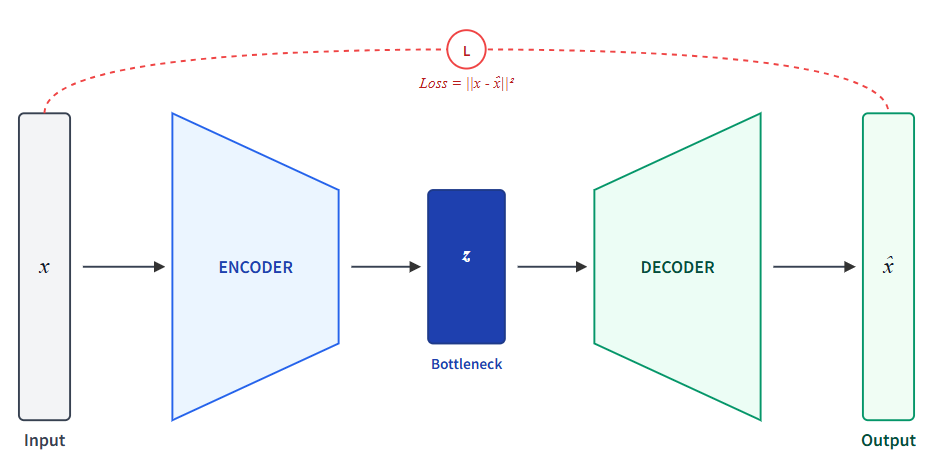
\includegraphics[width=1\linewidth]{chap1/image/Autoencoder.png}
\caption[Kiến trúc mạng nơ-ron tự mã hóa]{Kiến trúc tổng quát của mạng nơ-ron tự mã hóa.}
\label{fig:autoencoder_general}
\end{figure}

\subsection{Kiến trúc mạng Dense}

Mạng nơ-ron tự mã hóa Dense là cấu trúc cơ bản nhất của mạng tự mã hóa, trong đó mỗi nơ-ron đều được kết nối trực tiếp với toàn bộ nơ-ron ở tầng kế tiếp. Quá trình hoạt động của mạng Dense bao gồm hai giai đoạn chính. Đầu tiên, bộ mã hóa sử dụng hàm $f_{\phi}$ để ánh xạ vectơ đầu vào $x \in \mathbb{R}^d$ sang không gian ẩn $h \in \mathbb{R}^k$ (với $k < d$), như trong Phương trình \ref{eq:encoder}:

\begin{equation}\label{eq:encoder}h = \sigma(W_e x + b_e)\end{equation}

Sau đó, bộ giải mã dùng hàm $g_{\psi}$ để ánh xạ ngược từ không gian ẩn $h$ về lại không gian ban đầu, tạo ra tín hiệu phục hồi $\hat{x} \in \mathbb{R}^d$ theo Phương trình \ref{eq:decoder}:

\begin{equation}\label{eq:decoder}\hat{x} = \sigma'(W_d h + b_d)\end{equation}

Trong đó, $W_e, W_d$ là các ma trận trọng số; $b_e, b_d$ là các vectơ độ lệch (bias); và $\sigma, \sigma'$ là các hàm kích hoạt phi tuyến. Quá trình huấn luyện sẽ tối ưu hóa tập tham số $\phi$ và $\psi$ nhằm cực tiểu hóa sai số tái tạo trên dữ liệu bình thường. Với dữ liệu tín hiệu cảm biến chuỗi thời gian, hàm mất mát thường được sử dụng nhất là Sai số bình phương trung bình (Mean Squared Error - MSE):

\begin{equation}\label{eq:mse_loss}\mathcal{L}(\phi, \psi) = \frac{1}{n} \sum_{i=1}^{n} |x_i - g_{\psi}(f_{\phi}(x_i))|^2\end{equation}

Trong bài toán của đồ án, do vectơ đầu vào chỉ có kích thước 19 chiều (gồm các đặc trưng thống kê rung động và Năng lượng dải Mel - MFE\footnote{Mel-Filterbank Energy (MFE) là kỹ thuật xử lý tín hiệu âm thanh mô phỏng cách cảm nhận tần số của tai người, bằng cách nhóm các phổ tần số thu được từ biến đổi Fourier thành các dải năng lượng logarit. Chi tiết về phương pháp này sẽ được trình bày ở Mục \ref{subsec:audio_features}.}), cấu trúc Dense AE cực kỳ phù hợp. Kiến trúc nông và nhỏ gọn này giúp giải quyết hiệu quả bài toán tiết kiệm dung lượng bộ nhớ Flash và SRAM vốn rất hạn hẹp trên vi điều khiển \cite{ref_1_4}.

\subsection{Kiến trúc 1D-CNN và các giới hạn trên nền tảng nhúng}

Khác với Dense AE, mạng nơ-ron tích chập một chiều (1D-CNN) được thiết kế chuyên biệt để khai thác tính tương quan cục bộ trên dữ liệu chuỗi thời gian. Kiến trúc này sử dụng các bộ lọc (kernels) trượt dọc theo trục thời gian để trích xuất đặc trưng. Phép toán tích chập tại một vị trí $t$ với bộ lọc $w$ có kích thước $k$ được biểu diễn như Phương trình \ref{eq:conv1d}:

\begin{equation}\label{eq:conv1d}y_t = \sum_{i=0}^{k-1} w_i \cdot x_{t-i} + b\end{equation}

Về mặt lý thuyết, 1D-CNN AE rất hiệu quả trong việc nhận diện các mẫu rung động tuần hoàn hoặc các xung dị thường. Tuy nhiên, khi triển khai thực tế trên vi điều khiển, kiến trúc này bộc lộ những hạn chế lớn về mặt hiệu năng. Phép toán tích chập đòi hỏi số lượng lớn các phép nhân-cộng tích lũy (MACs), làm tăng độ trễ suy luận và tiêu tốn nhiều không gian bộ nhớ SRAM \cite{ref_1_1, ref_1_11}. Thêm vào đó, kết quả thực nghiệm của đề tài (sẽ được phân tích chi tiết tại Chương 4) còn chỉ ra một thách thức khác: sai số tái tạo của 1D-CNN AE biến động rất mạnh khi ép kiểu trọng số từ Float32 sang INT8. Điều này khiến hệ thống khó duy trì được độ tin cậy sau quá trình lượng tử hóa \cite{ref_1_1}.

\subsection{Lựa chọn kiến trúc tối ưu cho bài toán giám sát thiết bị gia dụng}

Thiết kế mô hình Trí tuệ nhân tạo tại biên (Edge AI) luôn là bài toán đánh đổi giữa độ nhạy phát hiện lỗi, độ trễ suy luận và tài nguyên bộ nhớ. Vì vậy, ở giai đoạn đầu, đồ án tiến hành so sánh ba kiến trúc mạng tự mã hóa trên môi trường mô phỏng Kaggle gồm Vanilla AE, 1D-CNN AE và LSTM AE. Các mô hình được huấn luyện trên cùng tập dữ liệu cảm biến đã tiền xử lý, sau đó được đánh giá theo sai số tái tạo, dung lượng sau lượng tử hóa INT8, độ trễ suy luận dự kiến tính toán trên Kaggle và mức ổn định khi thêm nhiễu.

Kết quả mô phỏng ban đầu xếp hạng hiệu quả theo thứ tự 1D-CNN AE, Vanilla AE và LSTM AE. Cần nhấn mạnh rằng các giá trị dung lượng và độ trễ trong giai đoạn này là số liệu dự kiến được tính toán trên Kaggle sau khi quy đổi/lượng tử hóa mô hình, chưa phải kết quả đo trực tiếp trên phần cứng. LSTM AE bị loại sớm do độ trễ suy luận dự kiến cao nhất, khoảng 129,50 ms, cùng dung lượng sau nén INT8 khoảng 368,66 KB. Vanilla AE có cấu trúc đơn giản hơn nhưng sai số tái tạo lớn nhất, với MSE đạt 0,004947, dung lượng INT8 dự kiến khoảng 375,01 KB và chỉ số bất ổn với nhiễu lên tới 793,63\%. Trong khi đó, 1D-CNN AE cho kết quả tốt nhất ở giai đoạn mô phỏng, với MSE 0,003698 và kích thước mô hình dự kiến khoảng 30,52 KB, nên ban đầu được xem là ứng viên chính cho hệ thống.

Tuy nhiên, khi chuyển sang giai đoạn triển khai trên TensorFlow Lite Micro, 1D-CNN AE bộc lộ các rào cản kỹ thuật nghiêm trọng. Kết quả suy luận giữa môi trường Python và C++ không khớp do khác biệt trong triển khai toán tử Conv1D; đầu vào dạng chuỗi làm tăng chi phí quản lý bộ đệm trên RAM; đồng thời quá trình lượng tử hóa INT8 gây rủi ro mất ổn định tham số. Từ kết quả này, đồ án chuyển sang hướng thiết kế Symmetric Dense AE kết hợp khối trích xuất đặc trưng DSP 19 chiều. Kiến trúc đối xứng giúp giảm độ phức tạp đồ thị suy luận, phù hợp hơn với giới hạn bộ nhớ của vi điều khiển Seeed Studio XIAO ESP32-S3 và trở thành kiến trúc cốt lõi cho hệ thống cuối cùng.

% ============================================================
% TÀI LIỆU THAM KHẢO TRÍCH DẪN CHO MỤC 1.2
% ============================================================
% \bibitem{ref_1_1} P. P. Ray, "A review on TinyML: State-of-the-art and prospects," 2022.
% \bibitem{ref_1_4} X. Wang et al., "Empowering Edge Intelligence: A Comprehensive Survey," 2025.
% \bibitem{ref_1_6} R. Chalapathy and S. Chawla, "DEEP LEARNING FOR ANOMALY DETECTION: A SURVEY," 2019.
% \bibitem{ref_1_10} O. K. Oyedotun and D. Aouada, "A CLOSER LOOK AT AUTOENCODERS FOR UNSUPERVISED ANOMALY DETECTION," 2022.
% \bibitem{ref_1_11} T. S. Ajani et al., "An Overview of Machine Learning within Embedded and Mobile Devices--Optimizations and Applications," Sensors, 2021.

\section{Công nghệ TinyML trên vi điều khiển}

TinyML (Tiny Machine Learning) là hướng tiếp cận đưa các mô hình học máy xuống thực thi trực tiếp trên các hệ thống nhúng và vi điều khiển với mức tiêu thụ điện năng chỉ vài miliwatt \cite{ref_1_1}. Việc tích hợp xử lý tín hiệu số (DSP) và mạng nơ-ron sâu ngay trên các thiết bị có tài nguyên hạn chế giúp dịch chuyển năng lực tính toán ra sát nguồn phát sinh dữ liệu. Phương pháp này giúp khắc phục hiệu quả các hạn chế về độ trễ, băng thông truyền tải và rủi ro bảo mật dữ liệu so với mô hình điện toán đám mây truyền thống \cite{ref_1_4}.

\subsection{Ràng buộc về tài nguyên phần cứng}

Triển khai mạng nơ-ron trên thiết bị biên như Seeed Studio XIAO ESP32-S3 yêu cầu tính toán kỹ lưỡng các giới hạn vật lý của phần cứng. Khác với môi trường đám mây, vi điều khiển phải đối mặt với ba rào cản thiết kế chính. Thứ nhất là giới hạn nghiêm ngặt về bộ nhớ, bao gồm bộ nhớ Flash để lưu trữ trọng số và bộ nhớ SRAM dành cho việc cấp phát tensor. Mặc dù ESP32-S3 sở hữu vi xử lý lõi kép Xtensa LX7 mạnh mẽ, dung lượng SRAM nội (internal SRAM) chỉ ở mức 512 KB \cite{ref_1_15}. Mức dung lượng này phải được chia sẻ đồng thời cho hệ điều hành, các ngăn xếp tác vụ (task stacks), bộ đệm truyền thông không dây và vùng nhớ cho mạng nơ-ron. Do đó, các mô hình học sâu buộc phải được nén tối ưu để tránh lỗi tràn bộ nhớ (Out of Memory) \cite{ref_1_11}.

Thứ hai là ràng buộc về độ trễ thực thi (Inference Latency). Trong bài toán giám sát máy giặt, tín hiệu rung động được lấy mẫu với tần số cao lên tới 1000 Hz. Điều này đòi hỏi mô hình phải hoàn thành quá trình suy luận (forward pass) trong một cửa sổ thời gian hẹp để đảm bảo tính thời gian thực, tránh gây thắt cổ chai dữ liệu. Cuối cùng là ràng buộc về năng lượng và năng lực xử lý; mô hình AI không được chiếm dụng quá nhiều chu kỳ CPU để đảm bảo hệ thống có thể duy trì đồng thời các tác vụ quản lý cảm biến và giao tiếp Wi-Fi/MQTT \cite{ref_1_1}.

\subsection{Kỹ thuật lượng tử hóa mô hình (Quantization INT8)}

Để vượt qua các giới hạn khắt khe về bộ nhớ và năng lực tính toán, lượng tử hóa nguyên 8-bit (INT8 Quantization) là kỹ thuật nén mô hình cốt lõi được áp dụng. Kỹ thuật này chuyển đổi các trọng số (weights) và giá trị kích hoạt (activations) từ định dạng số thực dấu phẩy động 32-bit (Float32) sang số nguyên 8-bit. Quá trình ánh xạ tuyến tính từ miền số thực $r$ sang miền số nguyên $q$ được mô tả qua Phương trình \ref{eq:quantization}:

\begin{equation}
\label{eq:quantization}
r = S(q - Z)
\end{equation}

Trong đó, $S$ (Scale) là số thực dương đại diện cho tỷ lệ thu phóng, và $Z$ (Zero-point) là giá trị số nguyên dùng để dịch tâm, tương ứng với giá trị 0 trong miền số thực \cite{ref_1_14}. Lượng tử hóa INT8 giúp giảm kích thước lưu trữ của mô hình đi khoảng 4 lần so với Float32, đồng thời giảm lượng RAM tĩnh tiêu thụ trong quá trình suy luận (inference) theo tỷ lệ tương ứng \cite{ref_1_1, ref_1_14}. Các nghiên cứu đã chỉ ra rằng khi kết hợp với phương pháp lượng tử hóa sau huấn luyện (Post-Training Quantization), mức suy giảm độ chính xác của mạng thường được kiểm soát dưới 1\% \cite{ref_1_14}. Hơn nữa, với kiến trúc lõi LX7 của ESP32-S3, dữ liệu kiểu INT8 cho phép vi điều khiển khai thác tối đa tập lệnh vector (Vector Instructions) chuyên dụng. Điều này giúp thực thi nhiều phép toán nhân-cộng tích lũy (MACs) song song, từ đó hệ thống có thể đạt được độ trễ suy luận khoảng 6,4 ms trên kiến trúc XIAO ESP32-S3 \cite{ref_1_4, ref_1_15}.

\subsection{Framework TensorFlow Lite for Microcontrollers}

Hệ thống sử dụng TensorFlow Lite for Microcontrollers (TFLite Micro) để nhúng trực tiếp mô hình tự mã hóa lượng tử hóa xuống vi điều khiển. TFLite Micro được thiết kế tối ưu cho các thiết bị biên, loại bỏ sự phụ thuộc vào hệ điều hành tiêu chuẩn và không yêu cầu cơ chế cấp phát bộ nhớ động. Việc không sử dụng các lệnh \texttt{malloc()} hay \texttt{new} trong quá trình chạy mô hình giúp ngăn ngừa rủi ro phân mảnh bộ nhớ, đảm bảo độ tin cậy cho hệ thống khi vận hành liên tục dài ngày \cite{ref_1_13}.

Framework này hoạt động bằng cách biên dịch mô hình thành một mảng byte không đổi (const byte array) lưu trên bộ nhớ Flash. Sau đó, một bộ thông dịch (Interpreter) sẽ điều phối quá trình tính toán thông qua một vùng đệm cấp phát sẵn duy nhất gọi là vùng đệm tensor (Tensor Arena) \cite{ref_1_13}. Việc tích hợp TFLite Micro trên hệ điều hành thời gian thực FreeRTOS cho phép hệ thống thực thi đa luồng độc lập. Dù tác vụ suy luận AI được gán mức ưu tiên thấp hơn các tác vụ thu thập dữ liệu phần cứng, kiến trúc đa nhân vẫn đảm bảo quá trình này đáp ứng tốt các yêu cầu về thời gian thực. Để mô hình TFLite Micro hoạt động chính xác, dữ liệu đầu vào cần đi qua một luồng xử lý tín hiệu số tối ưu, nội dung này sẽ được trình bày trong mục tiếp theo.

% --- Tài liệu tham khảo trích dẫn trong mục này ---
% \bibitem{ref_1_1} P. P. Ray, "A review on TinyML: State-of-the-art and prospects," 2022.
% \bibitem{ref_1_4} X. Wang et al., "Empowering Edge Intelligence: A Comprehensive Survey," 2025.
% \bibitem{ref_1_11} T. S. Ajani et al., "An Overview of Machine Learning within Embedded and Mobile Devices--Optimizations and Applications," Sensors, 2021.
% \bibitem{ref_1_13} Pete Warden and Daniel Situnayake, "TinyML: Machine Learning with TensorFlow Lite...", 2019.
% \bibitem{ref_1_14} B. Jacob et al., "Quantization and Training of Neural Networks...", CVPR 2018.
% \bibitem{ref_1_15} Espressif Systems, "ESP32-S3 Series Datasheet," Version 2.2, 2026.



\section{Cơ sở xử lý tín hiệu cảm biến}

Trong các hệ thống giám sát tại biên, tiền xử lý và trích xuất đặc trưng là bước quan trọng ảnh hưởng trực tiếp đến hiệu suất của mô hình. Thay vì đẩy trực tiếp dữ liệu thô với số chiều lớn vào mạng nơ-ron, quy trình trích xuất đặc trưng giúp giữ lại các thông tin cốt lõi, giảm nhiễu và hạ thấp đáng kể yêu cầu tính toán. Đối với bài toán giám sát máy giặt, hệ thống khai thác đồng thời hai nguồn dữ liệu: tín hiệu âm thanh để nhận diện biến động tần số cao và tín hiệu rung động để theo dõi trạng thái cơ khí ở tần số thấp.

\subsection{Trích xuất đặc trưng âm thanh}
\label{subsec:audio_features}

Tín hiệu âm thanh thu từ microphone INMP441 qua bus I2S có dạng chuỗi thời gian liên tục. Để mô hình tự mã hóa nhận diện được các âm thanh bất thường như lỗi ma sát hay tiếng rít động cơ, kỹ thuật năng lượng dải lọc Mel được áp dụng. Phương pháp này mô phỏng thính giác con người — nhạy cảm với các thay đổi ở dải tần số thấp hơn là tần số cao. Phép biến đổi từ tần số Hz sang thang đo Mel được tính theo Phương trình \ref{eq:mel_scale}:

\begin{equation}
\label{eq:mel_scale}
M(f) = 2595 \cdot \log_{10} \left( 1 + \frac{f}{700} \right)
\end{equation}

\begin{figure}[H]
\centering
\resizebox{\textwidth}{!}{%
\begin{tikzpicture}[
    node distance=0.55cm,
    block/.style={draw, rounded corners=2pt, align=center, minimum height=0.9cm, text width=2.25cm, font=\small},
    arrow/.style={->, thick}
]
\node[block] (raw) at (0,0) {Tín hiệu I2S\\âm thanh};
\node[block] (frame) at (2.8,0) {Chia khung\\512 mẫu};
\node[block] (hann) at (5.6,0) {Cửa sổ\\Hann};
\node[block] (fft) at (8.4,0) {FFT\\$|X(k)|^2$};
\node[block] (mel) at (11.2,0) {13 bộ lọc\\Mel};
\node[block] (log) at (14.0,0) {Log-energy\\MFE};
\draw[arrow] (raw) -- (frame);
\draw[arrow] (frame) -- (hann);
\draw[arrow] (hann) -- (fft);
\draw[arrow] (fft) -- (mel);
\draw[arrow] (mel) -- (log);
\end{tikzpicture}
}
\caption{Đường ống trích xuất đặc trưng âm thanh MFE.}
\label{fig:audio_mfe_pipeline}
\end{figure}

Quy trình xử lý trong Hình \ref{fig:audio_mfe_pipeline} bắt đầu bằng việc chia tín hiệu thành các khung dài 64 ms, tương đương 512 mẫu ở tần số lấy mẫu 8 kHz, trượt với bước nhảy 32 ms. Các tham số này được lựa chọn dựa trên sự cân bằng giữa khả năng giữ lại thông tin âm học và giới hạn tài nguyên của vi điều khiển. Tần số lấy mẫu 8 kHz cho phép giữ lại dải âm thanh 0--4 kHz theo định lý Nyquist, đủ bao phủ các thành phần tiếng ồn cơ khí chính của động cơ, vòng bi và lồng giặt, trong khi giảm đáng kể dung lượng bộ đệm và số phép tính so với các mức 16 kHz hoặc 44,1 kHz \cite{ref_shul_2023, ref_1_16}. Với 8 kHz, khung 512 mẫu tương ứng 64 ms và đồng thời là kích thước lũy thừa của 2, phù hợp để thực hiện FFT hiệu quả. Cấu hình này tạo độ phân giải tần số khoảng $8000/512 \approx 15{,}6$ Hz, đủ chi tiết để quan sát sự thay đổi phổ của tiếng ma sát hoặc tiếng rít cơ khí; nếu khung ngắn hơn, độ phân giải tần số giảm, còn nếu khung dài hơn, độ trễ và bộ nhớ đệm tăng không phù hợp với xử lý tại biên.

Bước nhảy 32 ms tạo mức chồng lấn 50\% giữa hai khung liên tiếp. Mức chồng lấn này giúp đặc trưng phổ thay đổi mượt hơn theo thời gian, hạn chế bỏ sót các bất thường ngắn nhưng vẫn không làm tăng gấp đôi tải tính toán như các mức chồng lấn dày hơn. Trước khi biến đổi, cửa sổ Hann được nhân với từng khung để làm mềm hai biên của đoạn tín hiệu, qua đó giảm hiện tượng rò rỉ phổ khi FFT giả định tín hiệu trong mỗi khung có tính tuần hoàn \cite{ref_1_16}. Nhờ vậy, các đặc trưng năng lượng Mel ổn định hơn và ít bị ảnh hưởng bởi nhiễu biên khung.

Sau đó, phép biến đổi Fourier nhanh (FFT) chuyển tín hiệu sang miền tần số, và phần năng lượng phổ được đưa qua dải 13 bộ lọc hình tam giác xếp chồng theo thang Mel \cite{ref_1_12}. Số lượng 13 bộ lọc được lựa chọn nhằm cân bằng giữa khả năng phân giải phổ và kích thước vectơ đầu vào. Giá trị này đủ để mô tả các vùng năng lượng chính của tiếng ồn cơ khí, đồng thời giữ không gian đặc trưng âm thanh ở mức nhỏ để khi kết hợp với 6 đặc trưng rung động, vectơ đầu vào cuối cùng chỉ có 19 chiều và phù hợp với vùng nhớ hạn chế của TensorFlow Lite Micro trên vi điều khiển.

Đầu ra của mỗi bộ lọc là một giá trị năng lượng logarit. Với bộ lọc Mel thứ $m$, đặc trưng năng lượng được tính theo Phương trình \ref{eq:mel_energy}:

\begin{equation}
\label{eq:mel_energy}
E_m = \log \left( \sum_{k=0}^{K-1} |X(k)|^2 H_m(k) + \epsilon \right)
\end{equation}

Trong đó, $X(k)$ là phổ sau FFT, $H_m(k)$ là đáp ứng của bộ lọc Mel thứ $m$, $K$ là số điểm tần số được xét và $\epsilon$ là hằng số nhỏ để tránh phép tính $\log(0)$. Đồ án chủ đích chọn MFE thay vì MFCC (Mel-Frequency Cepstral Coefficients) nhằm loại bỏ bước biến đổi Cosin ngược (DCT). Lựa chọn này giúp tiết kiệm chu kỳ CPU trên vi điều khiển trong khi vẫn bảo toàn đủ thông tin không gian phổ để phát hiện bất thường \cite{ref_1_1, ref_1_12}.

\subsection{Trích xuất đặc trưng rung động cơ học}

Tín hiệu rung động từ cảm biến gia tốc ADXL345 phản ánh trực tiếp các sự cố cơ học như mất cân bằng tải hay lệch trục lồng giặt. Vì các lỗi này thường bộc lộ rõ qua cường độ và độ phân tán của dao động trong miền thời gian, đồ án tiến hành trích xuất hai đặc trưng thống kê là Giá trị hiệu dụng (RMS) và Phương sai (Variance) cho từng trục (X, Y, Z).

Giá trị RMS đo lường mức năng lượng trung bình của rung động, được tính theo Phương trình \ref{eq:rms}:

\begin{equation}
\label{eq:rms}
x_{RMS} = \sqrt{\frac{1}{N} \sum_{i=1}^{N} x_i^2}
\end{equation}

Bên cạnh đó, Phương sai đánh giá mức độ biến thiên của tín hiệu quanh giá trị trung bình. Việc kết hợp phương sai giúp mô hình nhạy hơn với các xung va đập bất thường do mất cân bằng tải gây ra \cite{ref_1_3}. Công thức tính phương sai được mô tả tại Phương trình \ref{eq:variance}:

\begin{equation}
\label{eq:variance}
\sigma^2 = \frac{1}{N} \sum_{i=1}^{N} (x_i - \bar{x})^2
\end{equation}

Chỉ sử dụng các đặc trưng miền thời gian giúp hệ thống không phải tính toán các phép biến đổi miền phức tạp (như FFT), qua đó rút ngắn tối đa độ trễ suy luận và tiết kiệm dung lượng SRAM trên vi điều khiển Seeed Studio XIAO ESP32-S3 \cite{ref_1_11}.

\subsection{Kỹ thuật kết hợp dữ liệu đa phương thức}

Để đánh giá đầy đủ trạng thái vận hành của thiết bị, đồ án áp dụng kỹ thuật kết hợp dữ liệu ở mức đặc trưng. Phương pháp này giúp mô hình bắt được mối tương quan chéo giữa âm thanh và rung động; chẳng hạn, tiếng ồn tần số cao đi kèm với biên độ rung lớn thường là dấu hiệu rõ ràng của lỗi ở pha vắt.

Vectơ đầu vào $V_{input} \in \mathbb{R}^{19}$ được tạo ra bằng cách ghép các đặc trưng theo Phương trình \ref{eq:fusion}:

\begin{equation}
\label{eq:fusion}
V_{input} = [MFE_{1 \dots 13} \oplus RMS_{x,y,z} \oplus \sigma^2_{x,y,z}]
\end{equation}

Trong đó, toán tử $\oplus$ biểu diễn phép ghép nối, gộp không gian 13 chiều MFE và 6 chiều rung động thành một vectơ đặc trưng 19 chiều duy nhất.

Thao tác quan trọng nhất ở bước này là sử dụng \textbf{Chuẩn hóa hỗn hợp} để tinh chỉnh từng loại dữ liệu trước khi nạp vào mạng tự mã hóa. Với đặc trưng âm thanh MFE, do cường độ luôn bị giới hạn vật lý bởi độ nhạy của microphone, hệ thống dùng \textbf{Min-Max Scaling} để ánh xạ dải $[-80, 0]$ dB về khoảng $[0, 1]$. Ngược lại, dữ liệu rung động (RMS và phương sai) thường xuyên xuất hiện các đỉnh nhiễu cao đột biến khi có va đập. Để xử lý, hệ thống dùng \textbf{Robust Scaling} — phương pháp chuẩn hóa dựa trên trung vị và dải phân vị. Cách này đưa dữ liệu về cùng thang đo chuẩn mà không làm lu mờ thông tin của các đỉnh giá trị bất thường \cite{ref_1_8}.

Đường ống tiền xử lý và chuẩn hóa hỗn hợp này không chỉ cung cấp dữ liệu sạch cho mô hình trí tuệ nhân tạo mà còn là nền tảng để hệ thống chạy đa nhân song song ổn định trên FreeRTOS. Các nghiên cứu liên quan và những hạn chế mà hệ thống này khắc phục sẽ được tổng kết ở cuối chương.

% --- Ghi chú Tài liệu tham khảo ---
% \bibitem{ref_1_1} P. P. Ray, "A review on TinyML...", 2022.
% \bibitem{ref_1_3} H. Mohammadi, "EARLY DETECTION OF IMBALANCE IN LOAD...", 2020.
% \bibitem{ref_1_8} M. Abdallah et al., "Anomaly Detection and Inter-Sensor Transfer Learning on Smart Manufacturing Datasets," Sensors, 2023.
% \bibitem{ref_1_11} T. S. Ajani et al., "An Overview of Machine Learning within Embedded and Mobile Devices--Optimizations and Applications," Sensors, 2021.
% \bibitem{ref_1_12} U. Muthumala et al., "Comparison of Tiny Machine Learning Techniques for Embedded Acoustic Emission Analysis," IEEE WF-IoT, 2024.



\section{Các công trình liên quan và khoảng trống nghiên cứu}

\subsection{Các công trình liên quan trong lĩnh vực giám sát và phát hiện bất thường}

Giám sát tình trạng thiết bị và phát hiện bất thường cho các hệ thống máy móc là một bài toán quan trọng trong công nghiệp. Hầu hết các hệ thống giám sát Internet vạn vật hiện nay đều vận hành dựa trên kiến trúc điện toán đám mây. Trong đó, thiết bị biên đóng vai trò thu thập và truyền dữ liệu thô qua Internet về máy chủ để phân tích. Dù tận dụng được năng lực tính toán lớn, phương pháp này bộc lộ nhiều hạn chế khi áp dụng vào thiết bị gia dụng như: độ trễ phản hồi, sự phụ thuộc vào băng thông mạng, rủi ro rò rỉ dữ liệu cá nhân và chi phí hạ tầng \cite{ref_1_1, ref_1_4}.

Gần đây, sự phát triển của công nghệ TinyML đã thúc đẩy xu hướng dịch chuyển trí tuệ nhân tạo ra vùng biên. Nghiên cứu của Mansoureh Lord (2021) \cite{ref_1_lord} đã chứng minh tính khả thi của việc chạy trực tiếp các thuật toán học máy trên vi điều khiển nhằm phát hiện dị thường. Tác giả đã thử nghiệm kiến trúc mạng nơ-ron tự mã hóa và biến phân tự mã hóa (Variational Autoencoder - VAE), trong đó mô hình tự mã hóa đạt độ chính xác 92\% khi nhận diện lỗi qua sai số tái tạo. Bên cạnh đó, một số nghiên cứu cũng đã triển khai các thuật toán máy học truyền thống như máy véc-tơ hỗ trợ (Support Vector Machine - SVM) hay rừng ngẫu nhiên trên thiết bị biên để giám sát cơ khí thời gian thực \cite{ref_1_7}. 

Ở hướng học sâu không giám sát trên thiết bị gia dụng, Castangia và cộng sự (2022) \cite{ref_castangia_2022} đề xuất sử dụng VAE để phát hiện bất thường điện dựa trên chữ ký công suất của máy rửa bát, máy giặt và máy sấy. Nhóm tác giả tạo các điểm bất thường ngẫu nhiên nhằm mô phỏng lỗi điện thực tế, sau đó so sánh VAE với One-Class SVM sử dụng hai đặc trưng thủ công là năng lượng tiêu thụ và thời lượng chu kỳ. Kết quả cho thấy VAE đạt F1-Score lớn hơn 0,90 trên toàn bộ các thiết bị thử nghiệm, chứng minh lợi thế của học sâu trong việc mô hình hóa chu kỳ vận hành bình thường so với các đặc trưng thủ công.

Đối với riêng máy giặt, Shul và cộng sự (2023) \cite{ref_shul_2023} khai thác phổ tiếng ồn vận hành để phát hiện bất thường bằng mạng DNN tự giám sát. Công trình này nhấn mạnh rằng tiếng ồn của máy giặt thay đổi mạnh theo khối lượng đồ giặt và độ mất cân bằng, khiến bài toán phát hiện bất thường khó hơn trong điều kiện thực tế. Để xử lý bối cảnh vận hành, nhóm tác giả sử dụng thêm thông tin tốc độ quay của lồng và khối lượng đồ giặt, huấn luyện mô hình dự đoán phổ tiếng ồn tương lai từ các phổ quá khứ và kiểm chứng chéo trên nhiều loại vải, khối lượng khác nhau. Mô hình đề xuất cải thiện ROC-AUC tối đa khoảng 1,4\% trên toàn bộ tập kiểm thử, cho thấy tiềm năng của dữ liệu âm thanh nhưng vẫn đòi hỏi mô hình DNN phức tạp và thông tin vận hành nội bộ từ máy giặt.

Riêng với đối tượng máy giặt, các công trình hiện hành, tiêu biểu như của Mohammadi (2020) \cite{ref_1_3}, chủ yếu phân tích phổ rung động để phát hiện lỗi mất cân bằng tải. Tuy nhiên, các nghiên cứu này đa phần dựa trên học có giám sát – phương pháp đòi hỏi tập dữ liệu có nhãn lớn về các trạng thái lỗi. Điều này gây tốn kém chi phí và khó thực hiện trong điều kiện vận hành thiết bị gia dụng thực tế. 

Hơn nữa, việc đồng bộ hóa dữ liệu từ nhiều cảm biến (âm thanh, rung động) đòi hỏi năng lực xử lý tín hiệu cao. Trong các vi điều khiển đơn nhân, việc luân phiên giữa tác vụ đọc cảm biến liên tục và suy luận AI thường gây ra hiện tượng trôi thời gian (time drift), dẫn đến mất mát dữ liệu đầu vào khi hệ thống xử lý các tác vụ có mức ưu tiên xung đột nhau \cite{ref_1_11}.

\subsection{Khoảng trống nghiên cứu và đóng góp của đồ án}

Từ các phân tích trên, đồ án nhận diện ba khoảng trống nghiên cứu khi áp dụng TinyML vào bài toán Phát hiện bất thường cho máy giặt, qua đó đề xuất các giải pháp kỹ thuật cụ thể:

Thứ nhất, rào cản về cảnh báo giả do tính chất đa trạng thái của thiết bị. Máy giặt vận hành qua nhiều pha có đặc tính vật lý thay đổi liên tục. Do đó, đồ án đề xuất cơ chế Phân luồng đa trạng thái tự động (Chuyển đổi Ba trạng thái), giúp nhận diện pha vận hành theo thời gian thực từ dữ liệu chấn động, từ đó định tuyến dòng dữ liệu vào các mô hình học máy chuyên biệt (GENTLE, STRONG, SPIN). Hướng tiếp cận này giúp giảm thiểu tình trạng cảnh báo giả khi thiết bị chuyển pha.

Thứ hai, giới hạn về dữ liệu lỗi và không gian bộ nhớ của vi điều khiển. Đồ án áp dụng kiến trúc mạng nơ-ron đối xứng không giám sát \cite{ref_1_5}, chỉ yêu cầu học từ phân phối dữ liệu bình thường. Để tối ưu hóa cho vi điều khiển Seeed Studio XIAO ESP32-S3, kỹ thuật lượng tử hóa nhận thức huấn luyện được tích hợp, giúp nén dung lượng mô hình nhưng vẫn duy trì độ chính xác trên miền số nguyên INT8.

Thứ ba, thách thức về độ trễ và mất đồng bộ khi sử dụng đa cảm biến. Việc đồng thời trích xuất đặc trưng phổ âm thanh (I2S, Mel-filterbank) và đọc dữ liệu gia tốc (I2C) dễ làm gián đoạn luồng suy luận. Đồ án giải quyết vấn đề này bằng cách thiết kế hệ thống phần mềm xử lý song song thực sự trên nền tảng FreeRTOS. Tác vụ xử lý âm thanh được phân luồng vào lõi số 0, trong khi việc thu thập rung động và suy luận AI chạy trên lõi số 1. Dữ liệu giữa các luồng được đồng bộ hóa an toàn qua Nhóm sự kiện và Hàng đợi, ngăn ngừa hiện tượng thắt cổ chai phần cứng.

Thông qua việc giải quyết đồng thời ba vấn đề trên, hệ thống được đề xuất hướng tới việc đảm bảo tính chính xác và độ phản hồi theo thời gian thực, cung cấp một phương pháp tiếp cận phù hợp cho các ứng dụng trí tuệ nhân tạo tại biên đa phương thức.

% ==============================================================================
% DANH MỤC TÀI LIỆU THAM KHẢO TRÍCH DẪN (CHI TIẾT)
% ==============================================================================
% \bibitem{ref_1_1} P. P. Ray, "A review on TinyML: State-of-the-art and prospects," Journal of King Saud University - Computer and Information Sciences, vol. 34, no. 4, pp. 1595-1623, 2022.
% \bibitem{ref_1_lord} M. Lord, "TinyML Anomaly Detection," Master's thesis, Dept. Comput. Sci., California State Univ., Northridge, CA, USA, 2021.
% \bibitem{ref_1_3} H. Mohammadi, "Early Detection of Imbalance in Load and Machine in Front Load Washing Machines by Monitoring Drum Movement," Master's thesis, Sabancı University, Istanbul, Turkey, 2020.
% \bibitem{ref_1_4} X. Wang et al., "Empowering Edge Intelligence: A Comprehensive Survey on On-Device AI Models," arXiv preprint arXiv:2503.06027, 2025.
% \bibitem{ref_1_5} "Unsupervised Anomaly Detection for IoT-Based Multivariate Time Series: Existing Solutions, Performance Analysis and Future Directions," Sensors, vol. 23, no. 1, 2023.
% \bibitem{ref_1_7} E. Njor et al., "A Holistic Review of the TinyML Stack for Predictive Maintenance," IEEE Access, vol. 12, pp. 2450-2475, 2024.
% \bibitem{ref_1_11} T. S. Ajani et al., "An Overview of Machine Learning within Embedded and Mobile Devices--Optimizations and Applications," Sensors, 2021.
% \bibitem{ref_1_14} B. Jacob et al., "Quantization and Training of Neural Networks for Efficient Integer-Arithmetic-Only Inference," in Proc. IEEE Conf. Comput. Vis. Pattern Recognit. (CVPR), 2018, pp. 2704-2713.



\chapter{THIẾT KẾ HỆ THỐNG}
\label{chuong_2}

\section{Kiến trúc tổng thể hệ thống}

Hệ thống được thiết kế theo mô hình kiến trúc AIoT định hướng biên, tập trung vào khả năng xử lý tại chỗ nhằm đảm bảo tính thời gian thực. Cấu trúc hệ thống được chia thành bốn tầng chức năng chính để thuận tiện cho việc quản lý và mở rộng (Hình \ref{fig:system_architecture}).

\begin{figure}[p]
    \centering
    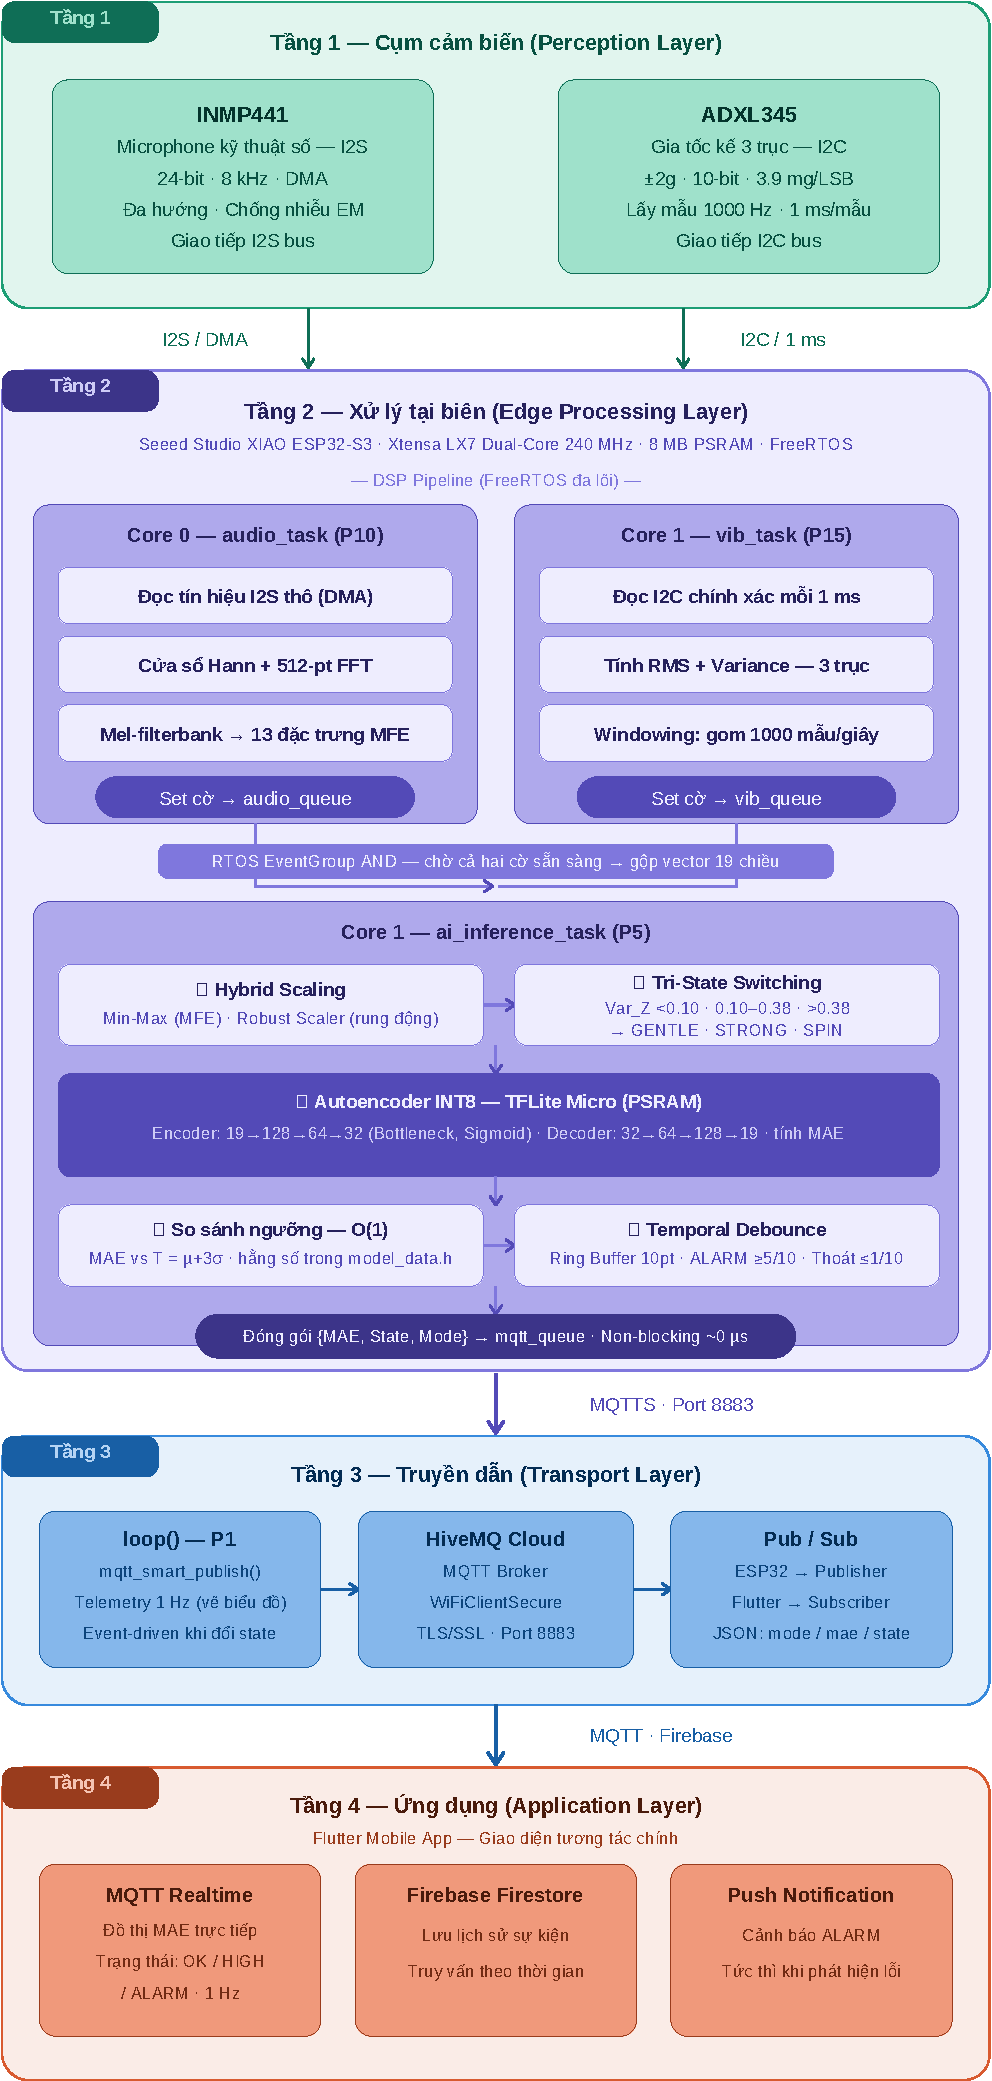
\includegraphics[width=0.65\linewidth]{chap2/image/kien_truc_4_tang_v4_cropped.pdf}
    \caption[Sơ đồ kiến trúc tổng thể hệ thống]{Sơ đồ kiến trúc tổng thể hệ thống bao gồm 4 tầng chức năng: Tầng cảm biến, Tầng xử lý tại biên, Tầng truyền dẫn và Tầng ứng dụng.}
    \label{fig:system_architecture}
\end{figure}

\subsection{Sơ đồ khối chức năng}

Các khối thành phần trong hệ thống tương tác theo luồng dữ liệu một chiều để tối ưu hóa thời gian phản hồi:

\begin{itemize}
    \item \textbf{Tầng cảm biến:} Gồm microphone kỹ thuật số INMP441 (I2S) thu tín hiệu âm thanh và cảm biến gia tốc ADXL345 (I2C) đo rung động cơ học của lồng giặt.
    
    \item \textbf{Tầng xử lý tại biên:} Sử dụng vi điều khiển Seeed Studio XIAO ESP32-S3 làm đơn vị xử lý trung tâm. Tại đây, dữ liệu thô được đưa qua đường ống xử lý tín hiệu số, trích xuất thành vector đặc trưng 19 chiều và nạp vào mô hình mạng nơ-ron tự mã hóa lượng tử hóa INT8 để suy luận \cite{ref_1_lord}. Hệ thống tận dụng kiến trúc lõi kép để thực hiện song song các tác vụ thu thập dữ liệu và tính toán mạng nơ-ron.
    
    \item \textbf{Tầng truyền dẫn:} Sử dụng giao thức MQTTS qua cổng 8883 để kết nối với HiveMQ Cloud. Đây là lớp trung gian điều phối thông tin từ thiết bị biên đến ứng dụng người dùng một cách bảo mật qua lớp mã hóa TLS/SSL.
    
    \item \textbf{Tầng ứng dụng:} Ứng dụng di động phát triển trên nền tảng Flutter đóng vai trò giao diện tương tác chính. Ứng dụng tích hợp đồng bộ dữ liệu thời gian thực qua MQTT và dữ liệu lịch sử qua Firebase Firestore. Cơ chế thông báo đẩy được sử dụng để cảnh báo người dùng kịp thời về các sự cố hỏng hóc.
\end{itemize}

\subsection{Đường ống xử lý luồng dữ liệu}

Quy trình xử lý dữ liệu được thiết kế theo cấu trúc luồng tuyến tính, đảm bảo tính toàn vẹn từ dữ liệu vật lý đến quyết định logic:

\begin{enumerate}
    \item Thu thập và Tiền xử lý: Tín hiệu âm thanh đi qua bộ lọc cửa sổ Hann và phép biến đổi Fourier nhanh 512 điểm để trích xuất 13 đặc trưng bộ lọc Mel. Song song đó, tín hiệu rung động (lấy mẫu ở tốc độ 1000 mẫu/giây) được tính toán giá trị hiệu dụng và phương sai để làm cơ sở phân tích trạng thái.
    
    \item Định tuyến trạng thái: Dựa trên phương sai trục Z của rung động, hệ thống tự động xác định máy đang vận hành ở pha nào (GENTLE, STRONG, hoặc SPIN). Từ đó, vi điều khiển thực hiện nạp và kích hoạt mô hình AI chuyên biệt tương ứng lên vùng đệm tensor.
    
    \item Suy luận AI và so sánh ngưỡng: Vector đặc trưng được đưa qua lớp chuẩn hóa kép trước khi vào mô hình mạng nơ-ron tự mã hóa để tính toán lỗi tái tạo (MAE). Hệ thống sử dụng các ngưỡng phát hiện dị thường đã được tối ưu hóa riêng biệt cho từng pha vận hành. Các giá trị này được nhúng trực tiếp dưới dạng hằng số tĩnh nhằm triệt tiêu độ trễ tính toán, cho phép nhận diện lỗi với độ phức tạp $\mathcal{O}(1)$.
    
    \item Hậu xử lý: Để triệt tiêu báo động giả do nhiễu cơ học tức thời, hệ thống áp dụng cơ chế bộ lọc cửa sổ trượt có nhớ và bộ đệm vòng lưu giữ 10 trạng thái gần nhất. Thuật toán trễ được tích hợp để thiết lập bộ quy tắc bất đối xứng: hệ thống chỉ chuyển sang trạng thái ALARM khi có ít nhất 5/10 mẫu vượt ngưỡng, và chỉ khôi phục về trạng thái bình thường khi tỷ lệ lỗi giảm xuống mức tối thiểu ($\le$ 1/10). Cơ chế có trạng thái này đảm bảo độ tin cậy tuyệt đối cho hệ thống.
\end{enumerate}

\subsection{Cơ chế điều phối đa nhiệm trên FreeRTOS}

Đồ án triển khai kiến trúc song song thực sự trên lõi kép của FreeRTOS nhằm triệt tiêu hiện tượng mất đồng bộ thời gian trong kỹ thuật kết hợp dữ liệu đa phương thức:

\begin{itemize}
    \item Lõi số 0: Chuyên trách tiền xử lý tín hiệu. Tác vụ audio\_task với mức ưu tiên 10 thực hiện đọc I2S và liên tục thực thi khối lệnh FFT/bộ lọc Mel nặng về tính toán dấu phẩy động.
    \item Lõi số 1: Đảm nhiệm hai tác vụ quan trọng. Tác vụ vib\_task được cấp đặc quyền cao nhất trong nhóm tác vụ người dùng với mức ưu tiên 15 nhằm đảm bảo chu kỳ lấy mẫu phần cứng I2C chính xác ở mức 1 ms. Tác vụ ai\_inference\_task với mức ưu tiên 5 chịu trách nhiệm vận hành mô hình TFLite Micro và chạy thuật toán phân tích cảnh báo.
\end{itemize}

Việc đồng bộ hóa giữa các lõi được thực thi qua cơ chế nhóm sự kiện (đảm bảo logic cổng AND - AI chỉ chạy khi cả hai cảm biến đã sẵn sàng) và hàng đợi luồng an toàn. Đặc biệt, hệ thống cô lập hoàn toàn khâu truyền dẫn mạng khỏi tiến trình AI. Tác vụ AI chỉ làm nhiệm vụ đóng gói cảnh báo và đẩy vào mqtt\_queue qua thao tác không chặn (mất $\sim$0 $\mu$s). Hàm loop() nội tại của vi điều khiển, chạy ngầm ở mức ưu tiên 1, đóng vai trò tiêu thụ dữ liệu từ hàng đợi này và xử lý các gián đoạn I/O mạng. Thiết kế này giúp triệt tiêu hoàn toàn rủi ro độ trễ mạng làm treo cứng tiến trình giám sát AI tại biên.

% ==============================================================================
% DANH MỤC TÀI LIỆU THAM KHẢO TRÍCH DẪN (CHI TIẾT CHO MỤC 2.1)
% Sao chép dòng dưới đây vào file .bib hoặc môi trường thebibliography của bạn
% ==============================================================================
% \bibitem{ref_1_lord} M. Lord, "TinyML Anomaly Detection," Master's thesis, Dept. Comput. Sci., California State Univ., Northridge, CA, USA, 2021.



\section{Thiết kế phần cứng}

Hệ thống phần cứng được thiết kế hướng tới sự nhỏ gọn và tiết kiệm năng lượng, đồng thời cần đảm bảo năng lực tính toán đủ để thực thi song song các luồng xử lý tín hiệu và mạng nơ-ron.

\subsection{Nền tảng vi điều khiển lõi kép XIAO ESP32-S3}

Trung tâm điều khiển và xử lý suy luận của hệ thống là mô-đun Seeed Studio XIAO ESP32-S3. Việc lựa chọn nền tảng này thay vì các dòng vi điều khiển truyền thống được dựa trên ba yếu tố kỹ thuật chính:

\begin{itemize}
    \item Kiến trúc đa nhân và tập lệnh gia tốc Trí tuệ nhân tạo (AI): Chip được trang bị vi xử lý Xtensa® 32-bit LX7 lõi kép hoạt động ở xung nhịp 240 MHz. Dòng S3 có hỗ trợ các tập lệnh mở rộng vector, giúp thực thi các phép toán nhân-tích lũy (MAC) hiệu quả hơn, phù hợp cho việc gia tốc suy luận với mô hình TensorFlow Lite Micro \cite{ref_1_15}.
    \item Hệ thống bộ nhớ phân tầng: Hệ thống sử dụng phiên bản có tích hợp sẵn 8 MB PSRAM (Pseudo-Static RAM) và 8 MB bộ nhớ Flash bên cạnh 512 KB SRAM nội bộ \citeweb{ref_2_xiao}. Dung lượng PSRAM mở rộng đóng vai trò là vùng đệm cho phép hệ thống nạp cùng lúc ba mô hình mạng nơ-ron tự mã hóa (GENTLE, STRONG, SPIN), hỗ trợ thiết bị chuyển đổi mô hình linh hoạt mà không gây quá tải bộ nhớ.
    \item Kết nối Internet vạn vật (IoT): Tích hợp sẵn Wi-Fi 2.4 GHz, cung cấp băng thông đủ để triển khai các giao thức truyền tải mã hóa (WiFiClientSecure) kết nối với máy chủ đám mây.
\end{itemize}

\subsection{Tích hợp microphone kỹ thuật số INMP441 qua chuẩn giao tiếp I2S}

Để thu thập đặc trưng âm thanh, hệ thống sử dụng microphone kỹ thuật số đa hướng INMP441. Đây là cảm biến MEMS có các đặc điểm phù hợp với môi trường dễ nhiễu động như máy giặt:

\begin{itemize}
    \item Giao tiếp I2S (Inter-IC Sound): Tín hiệu âm thanh được số hóa trực tiếp tại cảm biến với độ phân giải 24-bit và truyền về vi điều khiển Seeed Studio XIAO ESP32-S3 qua bus I2S \cite{ref_2_inmp441}. Cách tiếp cận này giúp hạn chế nhiễu điện từ môi trường — một vấn đề thường gặp ở các microphone analog khi hoạt động gần động cơ công suất lớn.
    \item Cơ chế truy cập bộ nhớ trực tiếp (DMA): Luồng dữ liệu âm thanh lấy mẫu ở tần số 8 kHz được đẩy thẳng vào vùng nhớ SRAM thông qua bộ điều khiển DMA. Kỹ thuật này giúp hệ thống thu thập dữ liệu liên tục mà không làm tăng đáng kể tải xử lý của CPU, cho phép lõi số 0 tập trung tài nguyên vào khâu tính toán đặc trưng bộ lọc Mel.
\end{itemize}

\subsection{Tích hợp cảm biến gia tốc ADXL345 qua chuẩn giao tiếp I2C}

Sự rung động vật lý của lồng giặt là dữ liệu quan trọng để nhận diện các trạng thái bất thường cơ học. Cảm biến gia tốc ba trục ADXL345 được tích hợp với cấu hình như sau:

\begin{itemize}
    \item Độ phân giải và dải đo: Cảm biến được thiết lập ở dải đo $\pm$2g. Với độ phân giải 10-bit (tương đương mức độ nhạy 3,9 mg/LSB) \cite{ref_2_adxl345}, thiết bị có thể ghi nhận được các biến động nhỏ của lồng giặt, hỗ trợ thu thập dữ liệu đầu vào ổn định.
    \item Tốc độ lấy mẫu 1000 Hz: Cảm biến giao tiếp qua bus I2C và được gán mức ưu tiên cao nhất trong hệ điều hành FreeRTOS (mức ưu tiên 15). Việc duy trì chu kỳ lấy mẫu 1 ms/mẫu giúp hệ thống tính toán chính xác giá trị hiệu dụng và phương sai của trục Z, làm cơ sở dữ liệu cho thuật toán phân luồng trạng thái tự động.
\end{itemize}

\subsection{Sơ đồ kết nối và bố trí thiết bị trên đối tượng nghiên cứu}

Việc bố trí thiết bị giám sát được thiết kế dựa trên thực nghiệm, tuân thủ sơ đồ nối dây phần cứng chi tiết (Hình \ref{fig:hardware_wiring}).

\begin{figure}[H]
    \centering
    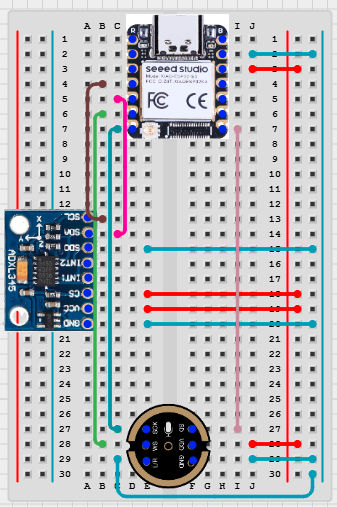
\includegraphics[width=0.3\linewidth]{chap2/image/SoDoNoiChan.png}
    \caption[Sơ đồ kết nối phần cứng]{Sơ đồ kết nối phần cứng và vị trí lắp đặt cụm cảm biến}
    \label{fig:hardware_wiring}
\end{figure}

Toàn bộ cụm mạch được đặt trong vỏ bảo vệ cách điện và gắn cố định tại mặt bên ngoài lồng giặt. Vị trí này được lựa chọn dựa trên hai yếu tố:
\begin{enumerate}
    \item Về mặt âm học: Hỗ trợ thu nhận tín hiệu âm thanh trực tiếp từ lồng máy, đồng thời giúp microphone giảm thiểu một phần các tạp âm nhiễu từ môi trường xung quanh.
    \item Về mặt cơ học: Các dao động do mất cân bằng tải hoặc lỗi trục sẽ được cảm biến gia tốc ghi nhận với biên độ rõ rệt nhất, qua đó cải thiện tỷ số tín hiệu trên nhiễu (SNR) của vector đặc trưng đầu vào.
\end{enumerate}

Với phần cứng và sơ đồ kết nối đã thiết lập, phần tiếp theo sẽ trình bày chi tiết về thiết kế phần mềm nhúng để điều phối các tác vụ và triển khai thuật toán Trí tuệ nhân tạo (AI) trên hệ thống.

% ==============================================================================
% DANH MỤC TÀI LIỆU THAM KHẢO TRÍCH DẪN (CHI TIẾT CHO MỤC 2.2)
% ==============================================================================
% \bibitem{ref_1_15} Espressif Systems, "ESP32-S3 Series Datasheet," Version 2.2, 2026.
% \bibitem{ref_2_xiao} Seeed Studio, "Getting Started with Seeed Studio XIAO ESP32S3 (Sense)," 2023. [Online]. Available: https://wiki.seeedstudio.com/xiao_esp32s3_getting_started/
% \bibitem{ref_2_inmp441} TDK InvenSense, "INMP441: Omnidirectional Microphone with Bottom Port and I2S Digital Output," Datasheet, 2014.
% \bibitem{ref_2_adxl345} Analog Devices, "3-Axis, ±2 g/±4 g/±8 g/±16 g Digital Accelerometer ADXL345," Datasheet, 2015.


\section{Kiến trúc phần mềm nhúng dựa trên hệ điều hành FreeRTOS}

Phần mềm nhúng của hệ thống được phát triển trên FreeRTOS để đáp ứng yêu cầu xử lý thời gian thực \cite{ref_2_freertos}. Trong các hệ thống nhúng đơn giản, cấu trúc vòng lặp tuần tự có thể đủ cho việc đọc cảm biến và điều khiển cơ bản. Tuy nhiên, hệ thống AIoT của đồ án phải thực hiện đồng thời nhiều tác vụ có đặc tính thời gian khác nhau, bao gồm thu thập dữ liệu âm thanh, lấy mẫu rung động, xử lý tín hiệu số, suy luận TensorFlow Lite Micro, duy trì kết nối Wi-Fi và truyền bản tin MQTT. Nếu toàn bộ luồng xử lý được đặt trong một vòng lặp duy nhất, độ trễ mạng hoặc tác vụ tính toán nặng có thể làm mất mẫu cảm biến và ảnh hưởng trực tiếp đến sai số tái tạo.

FreeRTOS cho phép chia hệ thống thành các tác vụ độc lập, mỗi tác vụ có mức ưu tiên và chu kỳ thực thi riêng. Thay vì sử dụng mô hình lập trình tuần tự, đồ án triển khai kiến trúc \textit{song song thực sự trên lõi kép}, khai thác hai lõi vật lý của Seeed Studio XIAO ESP32-S3 để phân tách độc lập luồng thu thập dữ liệu và luồng suy luận AI. Các cơ chế nhóm sự kiện, hàng đợi và ghim lõi được sử dụng nhằm đồng bộ dữ liệu, giảm tranh chấp tài nguyên và bảo vệ luồng suy luận khỏi độ trễ bất định của truyền thông mạng.

\subsection{Thiết kế luồng xử lý tín hiệu âm thanh trên lõi số 0}

Tác vụ xử lý âm thanh được gán vào lõi số 0 với mức ưu tiên 10, đảm bảo dòng dữ liệu liên tục và tránh mất mẫu. Đường ống xử lý bao gồm:

\begin{itemize}
    \item \textbf{Thu thập dữ liệu I2S-DMA:} Cơ chế DMA được sử dụng để đọc liên tục tín hiệu âm thanh từ microphone INMP441. Tần số lấy mẫu được thiết lập ở mức 8 kHz. Việc giới hạn tần số lấy mẫu này giúp tiết kiệm dung lượng bộ nhớ đệm và giảm tải khối lượng tính toán FFT, đồng thời vẫn giữ lại được các dải tần số âm học đặc trưng của động cơ (0-4 kHz).
    \item \textbf{Tiền xử lý DSP:} Tác vụ áp dụng hàm cửa sổ Hann và phép biến đổi Fourier nhanh 512 điểm thông qua thư viện \texttt{esp-dsp} \cite{ref_2_espdsp}.
    \item \textbf{Trích xuất đặc trưng Mel:} Năng lượng trên 13 dải lọc Mel được tính toán theo thang logarit để tạo thành vector đặc trưng âm thanh.
\end{itemize}

Sau khi hoàn tất, tác vụ sẽ đẩy dữ liệu vào \texttt{audio\_queue} và bật cờ hiệu \texttt{AUDIO\_READY\_BIT} trong nhóm sự kiện.

\subsection{Thiết kế luồng thu thập rung động và suy luận AI trên lõi số 1}

Lõi số 1 quản lý hai tác vụ với mức ưu tiên khác nhau, đảm nhiệm thu thập rung động và ra quyết định cảnh báo.

\textbf{Tác vụ thu thập rung động (\texttt{vib\_task}).} Tác vụ này được cấp mức ưu tiên cao nhất trong ứng dụng người dùng (mức ưu tiên 15) nhằm đảm bảo độ chính xác cho chu kỳ lấy mẫu. Thông qua hàm định thời \texttt{vTaskDelayUntil}, hệ thống duy trì chu kỳ 1 ms (1000 Hz) cho mỗi lần đọc cảm biến ADXL345 qua bus I2C. Dữ liệu sau đó được xử lý để lấy giá trị RMS và phương sai trục Z, đồng thời bật cờ hiệu \texttt{VIB\_READY\_BIT}.

\textbf{Tác vụ suy luận AI (\texttt{ai\_task}).} Được cấu hình ở mức ưu tiên 5, tác vụ này đảm nhiệm quá trình phân tích và ra quyết định với luồng thực thi như sau:
\begin{enumerate}
    \item \textbf{Đồng bộ hóa:} Đợi nhóm sự kiện (\texttt{AUDIO\_READY\_BIT} \& \texttt{VIB\_READY\_BIT}).
    \item \textbf{Chuẩn hóa hỗn hợp:} Áp dụng \textit{MinMax Scaling} cho 13 đặc trưng âm thanh và \textit{RobustScaler} cho 6 đặc trưng rung động để hạn chế ảnh hưởng của nhiễu ngoại lai trước khi suy luận.
    \item \textbf{Chuyển đổi bộ thông dịch:} Hệ thống đã cấp phát sẵn 3 vùng đệm tensor trên PSRAM. Dựa vào chỉ số phương sai rung động, hệ thống sẽ trỏ đến bộ thông dịch của mô hình tương ứng (GENTLE, STRONG, hoặc SPIN).
    \item \textbf{Suy luận:} Gọi hàm \texttt{Invoke()} của TensorFlow Lite Micro để tính toán sai số tái tạo (MAE).
    \item \textbf{Ra quyết định:} Đối chiếu giá trị MAE với các ngưỡng tĩnh đã được định nghĩa trong \texttt{model\_data.h} để xác định trạng thái bất thường.
\end{enumerate}

\subsection{Cơ chế đồng bộ hóa đa tác vụ}

Để quản lý luồng dữ liệu, hệ thống sử dụng ba cơ chế đồng bộ hóa của FreeRTOS:

\begin{itemize}
    \item \textbf{Nhóm sự kiện:} Đường ống xử lý AI chỉ được kích hoạt khi cả hai luồng dữ liệu (âm thanh và rung động) đều đã thu thập đủ mẫu, giúp loại bỏ tình trạng lệch pha thời gian giữa các cảm biến.
    \item \textbf{Hàng đợi:} Sử dụng \texttt{audio\_queue} để truyền vector đặc trưng và \texttt{mqtt\_queue} để truyền thông báo cảnh báo. Cơ chế hàng đợi giúp các tác vụ giao tiếp an toàn mà không chặn lẫn nhau.
    \item \textbf{Cô lập tác vụ truyền dẫn:} Quá trình gửi dữ liệu MQTTS được tách biệt khỏi luồng suy luận AI và đưa vào hàm \texttt{loop()} nội tại (mức ưu tiên 1). Hệ thống sử dụng phương thức \texttt{mqtt\_smart\_publish()} để gửi bản tin nhịp định kỳ (30 giây) hoặc gửi ngay lập tức khi có sự kiện cảnh báo. Cách thiết kế này tách biệt độ trễ mạng khỏi vòng lặp xử lý AI tại vùng biên, tránh gián đoạn quá trình suy luận.
\end{itemize}

% ==============================================================================
% DANH MỤC TÀI LIỆU THAM KHẢO TRÍCH DẪN (CHI TIẾT CHO MỤC 2.3)
% ==============================================================================
% \bibitem{ref_2_freertos} Real-Time Engineers Ltd., "FreeRTOS Reference Manual," v10.4.0, 2021. [Online]. Available: https://www.freertos.org
% \bibitem{ref_2_espdsp} Espressif Systems, "ESP-DSP Library Programming Guide," 2023. [Online]. Available: https://docs.espressif.com/projects/esp-dsp/


\section{Đề xuất kiến trúc phân mảnh trạng thái}

Máy giặt là một hệ thống động lực học có tính chu kỳ, trong đó các pha vận hành mang đặc tính vật lý (âm thanh và biên độ rung) thay đổi rõ rệt. Việc sử dụng một mô hình mạng nơ-ron tự mã hóa duy nhất để bao quát toàn bộ chu kỳ sẽ làm tăng độ phức tạp của không gian phân phối dữ liệu, dẫn đến tỷ lệ cảnh báo giả (False Positive) cao tại các thời điểm thiết bị chuyển pha. Các nghiên cứu trước đây thường chỉ tập trung giám sát trên một trạng thái tĩnh nhất định, bỏ qua vấn đề này \cite{ref_1_lord}. Để giải quyết bài toán này, đồ án đề xuất kiến trúc mạng nơ-ron tự mã hóa Ba trạng thái.

\subsection{Cơ sở phân tách chu trình hoạt động}

Để hệ thống có thể tự xác định trạng thái vận hành cục bộ mà không cần can thiệp vào mạch điều khiển trung tâm của máy giặt, một thuật toán phân luồng trạng thái dựa trên dữ liệu chấn động đã được thiết kế.

Thông qua phân tích tương quan thực nghiệm trên tập dữ liệu thu thập, nghiên cứu xác định được \textbf{phương sai trục Z} (đại diện cho cường độ chấn động thẳng đứng) của cảm biến ADXL345 là chỉ báo ổn định để phân loại trạng thái. Logic định tuyến được xây dựng bằng cách so sánh với các ngưỡng phân hoạch tĩnh, chia chu kỳ thành ba giai đoạn chính: \textbf{GENTLE} (Giặt/Ngâm), \textbf{STRONG} (Xả/Đảo lồng) và \textbf{SPIN} (Vắt tốc độ cao).

Các ngưỡng này được trích xuất từ phân tích phân phối thống kê của tập dữ liệu huấn luyện (trình bày chi tiết tại Chương 3). Cơ chế định tuyến này cho phép tác vụ \texttt{ai\_task} tự động trỏ con trỏ bộ thông dịch (\texttt{Interpreter}) tới vùng nhớ chứa trọng số mô hình tương ứng. Do cả ba mô hình đã được nạp sẵn trên PSRAM, quá trình chuyển đổi diễn ra tức thời, đáp ứng yêu cầu thời gian thực của hệ thống.

\subsection{Thiết kế mạng tự mã hóa Dense chuyên biệt}

Mỗi mô hình con được xây dựng theo kiến trúc mạng nơ-ron tự mã hóa Dense với cấu trúc đối xứng, giúp đơn giản hóa tính toán và cho phép tái sử dụng bộ đệm hiệu quả trong môi trường nhúng:

\begin{figure}[H]
\centering
\resizebox{0.98\textwidth}{!}{%
\begin{tikzpicture}[
    layer/.style={draw, rounded corners=2pt, align=center, minimum width=1.55cm, minimum height=1.0cm, font=\small},
    arrow/.style={->, thick}
]
\node[layer, fill=blue!8] (in) at (0,0) {Đầu vào\\19};
\node[layer, fill=green!10] (e1) at (2.0,0) {Dense\\128};
\node[layer, fill=green!10] (e2) at (4.0,0) {Dense\\64};
\node[layer, fill=orange!18] (b) at (6.0,0) {Cổ chai\\32};
\node[layer, fill=green!10] (d1) at (8.0,0) {Dense\\64};
\node[layer, fill=green!10] (d2) at (10.0,0) {Dense\\128};
\node[layer, fill=blue!8] (out) at (12.0,0) {Đầu ra\\19};
\draw[arrow] (in) -- (e1);
\draw[arrow] (e1) -- (e2);
\draw[arrow] (e2) -- (b);
\draw[arrow] (b) -- (d1);
\draw[arrow] (d1) -- (d2);
\draw[arrow] (d2) -- (out);
\node[font=\small] at (3.0,-0.9) {Khối mã hóa};
\node[font=\small] at (9.0,-0.9) {Khối giải mã};
\end{tikzpicture}
}
\caption{Kiến trúc mạng tự mã hóa Dense đối xứng dùng cho mỗi pha vận hành.}
\label{fig:symmetric_dense_ae_arch}
\end{figure}

\begin{itemize}
    \item \textbf{Lớp đầu vào:} Tiếp nhận vector đặc trưng 19 chiều (13 đặc trưng Mel-filterbank và 6 đặc trưng rung động).
    \item \textbf{Khối mã hóa:} Thực hiện nén dữ liệu qua các lớp ẩn ($19 \rightarrow 128 \rightarrow 64 \rightarrow 32$). Lớp ẩn đầu tiên được thiết kế theo hướng biểu diễn vượt quá nhằm tăng cường khả năng trích xuất các tương quan phi tuyến từ luồng tín hiệu đa phương thức \cite{ref_2_overcomplete}.
    \item \textbf{Khối giải mã:} Có cấu trúc phản chiếu đối xứng ($32 \rightarrow 64 \rightarrow 128 \rightarrow 19$), làm nhiệm vụ tái tạo lại vector đầu vào ban đầu.
\end{itemize}

\subsection{Kỹ thuật cân bằng đặc trưng với hàm mất mát MAE có trọng số}

Trong kỹ thuật kết hợp dữ liệu đa phương thức, sự chênh lệch về số lượng đặc trưng (13 chiều âm thanh so với 6 chiều rung động) có thể khiến thuật toán học máy ưu tiên giảm thiểu sai số của luồng âm học và bỏ qua các biến động cơ học nhỏ. Để khắc phục, đồ án áp dụng kỹ thuật hàm mất mát MAE có trọng số trong giai đoạn huấn luyện. Hàm mất mát được định nghĩa như sau:
\begin{equation}
    L_{WMAE} = \frac{1}{N} \sum_{i=1}^{N} w_i \cdot |x_i - \hat{x}_i|
\end{equation}
Trong đó, hệ số $w_i$ được đặt bằng $1$ đối với các đặc trưng âm thanh và bằng $5$ đối với các đặc trưng rung động. Giá trị 5 được lựa chọn theo hướng thực nghiệm có kiểm soát: nó bù lại bất lợi về số chiều của nhánh rung động (6 chiều so với 13 chiều âm thanh) nhưng vẫn không làm triệt tiêu hoàn toàn đóng góp của phổ âm thanh. Bằng cách tăng trọng số phạt trên sai số tái tạo của rung động, mô hình được định hướng biểu diễn chính xác hơn các đặc trưng cơ học, từ đó cải thiện độ nhạy với các sự cố bất thường vật lý. Hiệu quả của lựa chọn này được kiểm chứng trong nghiên cứu loại bỏ thành phần ở Chương 4, khi biến thể không dùng MAE có trọng số cho kết quả thấp hơn rõ rệt so với mô hình đề xuất.

\subsection{Đánh giá tương thích hàm kích hoạt trong môi trường lượng tử hóa}

Để triển khai hiệu quả trên vi điều khiển Seeed Studio XIAO ESP32-S3, phương pháp lượng tử hóa nhận thức huấn luyện được tích hợp. Kỹ thuật này ánh xạ toàn bộ trọng số mạng nơ-ron từ định dạng số thực Float32 sang định dạng số nguyên INT8.

Đặc biệt, tại lớp thắt cổ chai, đồ án sử dụng hàm kích hoạt Sigmoid thay cho hàm ReLU truyền thống. Quyết định thiết kế này dựa trên đặc tính hữu hạn của Sigmoid (giới hạn đầu ra trong khoảng $[0, 1]$). Khoảng giá trị này giúp quá trình lượng tử hóa ánh xạ đồng đều hơn vào 256 mức rời rạc của chuẩn INT8, qua đó giảm sai số mất mát thông tin so với hàm ReLU có dải giá trị dương không giới hạn \cite{ref_1_14}.

% ==============================================================================
% DANH MỤC TÀI LIỆU THAM KHẢO TRÍCH DẪN (CHI TIẾT CHO MỤC 2.4)
% ==============================================================================
% \bibitem{ref_1_lord} M. Lord, "TinyML Anomaly Detection," Master's thesis, CSUN, 2021.
% \bibitem{ref_2_overcomplete} Y. Bengio, A. Courville, and P. Vincent, "Representation Learning: A Review and New Perspectives," IEEE Trans. Pattern Anal. Mach. Intell., vol. 35, no. 8, pp. 1798-1828, 2013.
% \bibitem{ref_1_14} B. Jacob et al., "Quantization and Training of Neural Networks for Efficient Integer-Arithmetic-Only Inference," CVPR, 2018.


\section{Thiết kế hạ tầng truyền thông Internet of Things}

Hệ thống yêu cầu một hạ tầng mạng ổn định và tiết kiệm tài nguyên để truyền kết quả suy luận từ thiết bị biên đến người dùng. Đồ án sử dụng giao thức MQTT làm nền tảng giao tiếp, kết hợp với các cơ chế điều phối luồng tin phù hợp với giới hạn của vi điều khiển Seeed Studio XIAO ESP32-S3.

MQTT là giao thức truyền thông điệp gọn nhẹ, hoạt động theo mô hình xuất bản - đăng ký và được chuẩn hóa bởi OASIS cho các hệ thống IoT \citeweb{ref_mqtt_oasis}. Thay vì yêu cầu thiết bị biên kết nối trực tiếp đến từng ứng dụng người dùng, MQTT sử dụng một máy chủ trung gian để tiếp nhận, định tuyến và phân phối bản tin theo chủ đề. Cơ chế này giúp giảm độ phụ thuộc giữa thiết bị gửi và thiết bị nhận, đồng thời phù hợp với các nút mạng tài nguyên hạn chế nhờ kích thước bản tin nhỏ và chi phí duy trì kết nối thấp \citeweb{ref_hivemq_docs}.

\subsection{Mô hình xuất bản - đăng ký (Publish/Subscribe) và Broker}
Thay vì truyền tải dữ liệu cảm biến thô lên đám mây, kiến trúc trí tuệ nhân tạo tại biên cho phép thiết bị biên giữ lại vai trò xử lý tính toán. Nút mạng Seeed Studio XIAO ESP32-S3 đóng vai trò là một \textit{Publisher}, chỉ xuất bản các kết quả đã qua suy luận.

Hệ thống sử dụng HiveMQ Cloud làm dịch vụ máy chủ MQTT trung gian. Ứng dụng di động Flutter đóng vai trò là \textit{Subscriber}, đăng ký các chủ đề (Topic) cụ thể để nhận thông tin từ máy giặt. Mô hình xuất bản - đăng ký tách biệt logic hoạt động giữa thiết bị vật lý và phần mềm giám sát, giúp hai thành phần có thể phát triển độc lập.

\subsection{Cấu trúc bản tin chuẩn hóa JSON}
Dữ liệu giám sát được đóng gói theo định dạng JSON để tương thích đa nền tảng. Bản tin được thiết kế tối giản nhằm giảm overhead khi phân giải chuỗi (parsing) trên vi điều khiển, bao gồm 3 trường thông tin:
\begin{itemize}
    \item \texttt{mode}: Trạng thái vận hành hiện tại của máy giặt (GENTLE, STRONG, hoặc SPIN).
    \item \texttt{mae}: Giá trị sai số tái tạo do mô hình tự mã hóa xuất ra.
    \item \texttt{state}: Trạng thái đánh giá của hệ thống sau bộ lọc thời gian (OK, HIGH, hoặc ALARM).
\end{itemize}

\subsection{Kỹ thuật truyền tin hỗn hợp: Telemetry định kỳ và Hướng sự kiện}
Để cân bằng giữa yêu cầu trực quan hóa dữ liệu trên ứng dụng và giới hạn tài nguyên mạng, hệ thống triển khai hàm \texttt{mqtt\_smart\_publish()} tích hợp hai cơ chế truyền tin:

\begin{enumerate}
    \item \textbf{Truyền tin định kỳ (Dữ liệu đo xa 1 Hz):} Hệ thống thiết lập chu kỳ xuất bản bản tin 1 giây/lần. Tần số này đủ để cung cấp đồ thị sai số tái tạo (MAE) mượt mà trên ứng dụng giám sát thời gian thực, đồng thời không gây quá tải cho các tác vụ xử lý mạng của vi điều khiển.

    \item \textbf{Truyền tin hướng sự kiện:} Khi thuật toán nhận diện có sự thay đổi về trạng thái \texttt{state} (ví dụ: chuyển từ OK sang ALARM), một bản tin ngắt sẽ được xuất bản ngay lập tức mà không chờ đến chu kỳ tiếp theo, giữ độ trễ cảnh báo ở mức thấp nhất có thể.
\end{enumerate}

\subsection{Bảo mật truyền tải và Đánh đổi tài nguyên (Trade-offs)}
Hệ thống kết nối với Broker thông qua cổng 8883 để sử dụng giao thức MQTTS (MQTT qua TLS/SSL). Tuy nhiên, do phần lớn RAM của vi điều khiển Seeed Studio XIAO ESP32-S3 đã được cấp phát cho Tensor Arena của các mô hình AI, hệ thống cấu hình lớp \texttt{WiFiClientSecure} ở chế độ \texttt{setInsecure()}.

Phương pháp này vẫn mã hóa tải trọng (khối dữ liệu) trên đường truyền, nhưng bỏ qua bước xác thực chứng chỉ máy chủ Broker \cite{ref_2_tls_iot}. Đây là sự đánh đổi phù hợp với điều kiện tài nguyên hạn chế của phần cứng hiện tại; việc tích hợp xác thực chứng chỉ đầy đủ được xác định là hướng mở rộng cho các phiên bản phần cứng sau.

% \bibitem{ref_2_tls_iot} M. Frustaci, G. Pace, G. Aloi, and G. Fortino, "Evaluating Critical Security Issues of the IoT World: Present and Future Challenges," IEEE Internet of Things Journal, vol. 5, no. 4, pp. 2483-2495, 2018.


\chapter{XÂY DỰNG DỮ LIỆU VÀ HUẤN LUYỆN MÔ HÌNH}
\label{chuong_3}

Trong các hệ thống học máy tại biên (TinyML), tập dữ liệu huấn luyện chất lượng cao là yếu tố nền tảng để mô hình hoạt động tốt trên thực tế. Do bài toán phát hiện bất thường gặp vấn đề khan hiếm dữ liệu lỗi, đề tài tiếp cận theo hướng học không giám sát, yêu cầu một tập dữ liệu nền (Background Dataset) chuẩn xác phản ánh các trạng thái vận hành bình thường của thiết bị. Chương này trình bày quy trình xây dựng tập dữ liệu thực tế, các kỹ thuật tăng cường dữ liệu và quá trình huấn luyện mô hình tự mã hóa ba trạng thái.

\section{Quá trình thu thập dữ liệu thực tế}

Để xây dựng tập dữ liệu phản ánh đặc tính vật lý của máy giặt, một trạm thu thập dữ liệu chuyên dụng dựa trên vi điều khiển Seeed Studio XIAO ESP32-S3 đã được thiết kế và gắn trực tiếp lên lồng giặt để đo đạc thực địa.

\subsection{Xây dựng giao thức truyền nhận dữ liệu tốc độ cao định dạng nhị phân}

Thu thập dữ liệu đa cảm biến (âm thanh 8 kHz + gia tốc 1 kHz) qua cổng Serial bằng văn bản ASCII sẽ gây độ trễ phân giải cao, dẫn đến tràn bộ đệm và mất mẫu. Để khắc phục, đồ án triển khai giao thức truyền dẫn nhị phân (Binary Protocol) tùy chỉnh qua UART ở tốc độ baud 921600. ESP32 trích xuất vector đặc trưng 19 chiều tại thiết bị biên, sau đó đóng gói vào một cấu trúc chuẩn:

\begin{itemize}
    \item \textbf{Cấu trúc Payload:} Mỗi gói tin bắt đầu bằng hai byte đồng bộ (Sync word) \texttt{0xAA 0xBB}, tiếp theo là 19 giá trị float (76 bytes), và kết thúc bằng một byte kiểm tra lỗi (Checksum).
    \item \textbf{Hiệu năng:} Truyền trực tiếp khối nhớ nhị phân thay vì chuyển đổi sang chuỗi tiết kiệm khoảng 60\% băng thông kênh truyền, đảm bảo thu thập liên tục mà không quá tải phần cứng.
\end{itemize}

\subsection{Tự động hóa quy trình thu thập và kiểm soát chất lượng dữ liệu}

Một kịch bản Python (\texttt{dataCollection.py}) được phát triển để tự động hóa quy trình thu thập cho các chu kỳ kéo dài 45 - 90 phút.

\begin{itemize}
    \item \textbf{Tự động hóa phân mảnh (Windowing):} Kịch bản liên tục đọc luồng Serial, căn lề theo byte đồng bộ để giải mã mảng nhị phân. Mỗi tệp ghi 5 giây được tách thành 5 cửa sổ 1 giây, tương ứng 5 mẫu đặc trưng độc lập, rồi lưu trữ dưới định dạng ma trận NumPy (\texttt{.npy}).
    \item \textbf{Kiểm soát chất lượng (Data Quality Control):} Quá trình thu nhận thực hiện hai bước kiểm tra:
    \begin{enumerate}
        \item \textit{Xử lý nhiễu:} Tự động loại bỏ các mẫu chứa giá trị \texttt{NaN} hoặc \texttt{Inf} (do xung đột bus I2C hoặc nhiễu điện từ).
        \item \textit{Đồng bộ hóa dải năng lượng:} Áp dụng kỹ thuật \textit{Audio Volume Shifting}, giới hạn năng lượng phổ Mel trong dải chuẩn $[-80, 0]$ dB. Thao tác này giúp khắc phục sai lệch biểu diễn dữ liệu giữa môi trường huấn luyện (Python) và môi trường thực thi (C++).
    \end{enumerate}
\end{itemize}

\subsection{Thống kê phân phối và xử lý sự mất cân bằng dữ liệu (Data Imbalance)}
\label{subsec:data_distribution_balance}

Sau nhiều phiên đo đạc các chu trình giặt thực tế, hệ thống có tập dữ liệu gốc (Raw Dataset) gồm 14.000 mẫu (khoảng 20 giờ vận hành). Dữ liệu được phân nhóm tự động thành ba cụm trạng thái dựa trên phương sai trục Z (Hình~\ref{fig:varZ_tristate}), phản ánh mất cân bằng tự nhiên của chu trình giặt:

\begin{itemize}
    \item \textbf{Tập GENTLE (Pha giặt/ngâm):} 12.853 mẫu (khoảng 91,8\%). Tỷ trọng lớn phù hợp vì đây là pha chiếm thời gian dài nhất.
    \item \textbf{Tập STRONG (Pha xả/đảo lồng):} 551 mẫu (3,9\%). Pha này diễn ra trong thời gian ngắn khi máy đảo lồng để xả nước.
    \item \textbf{Tập SPIN (Pha vắt):} 596 mẫu (4,3\%). Pha vắt tốc độ cao kéo dài vài phút ở cuối chu trình.
\end{itemize}

\begin{figure}[H]
    \centering
    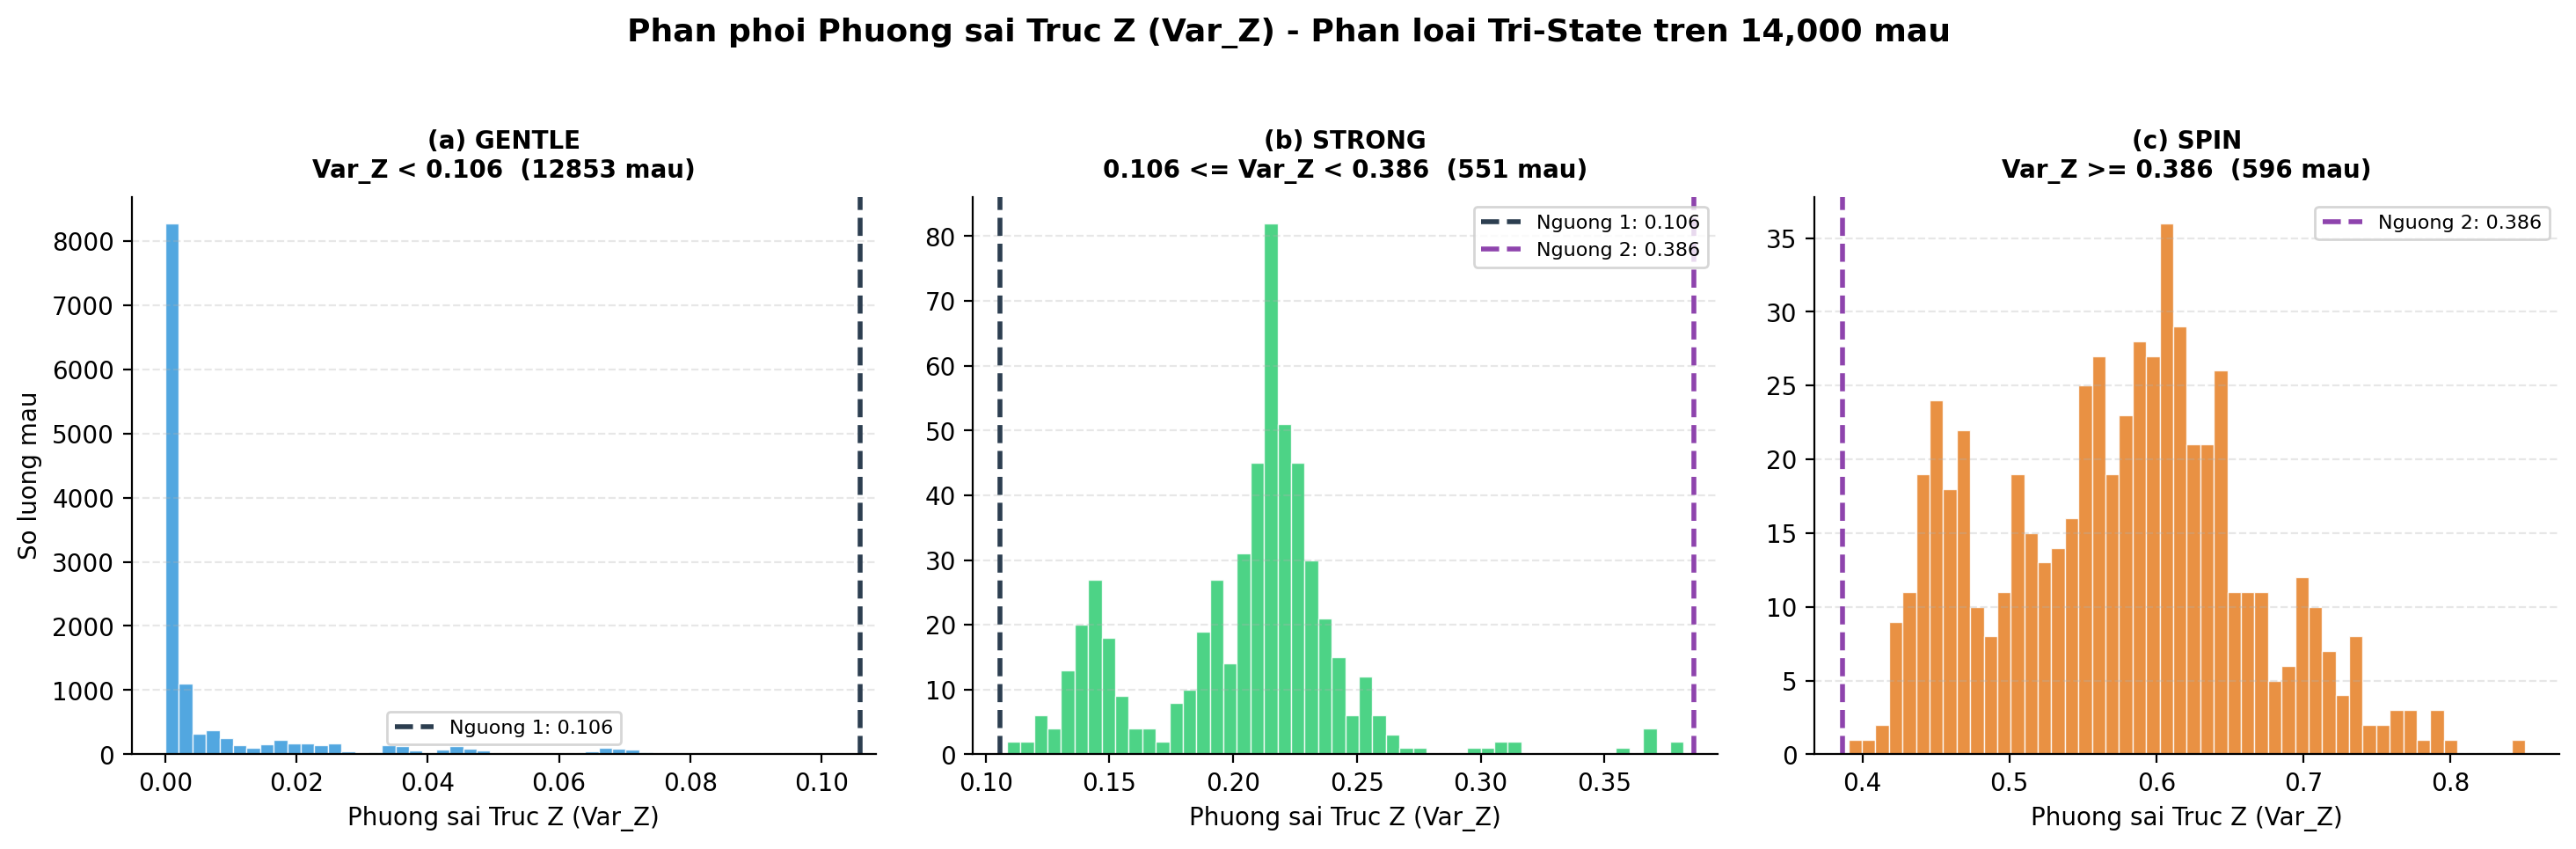
\includegraphics[width=0.95\linewidth]{chap3/image/fig_varZ_tristate.png}
    \caption[Phân phối phương sai trục Z]{Phân phối thực nghiệm của phương sai trục Z ($Var\_Z$) trên tập dữ liệu 14.000 mẫu. Hai ngưỡng phân hoạch tại 0.106 và 0.386 tạo ra ba vùng phân bố tách biệt rõ rệt.}
    \label{fig:varZ_tristate}
\end{figure}

Các ngưỡng phân hoạch trạng thái được xác định tự động thông qua thuật toán \textbf{K-Means Clustering}. Thuật toán gom cụm phương sai trục Z thành 3 nhóm, từ đó tính toán các ranh giới $\tau_1$ và $\tau_2$ tại điểm trung vị giữa hai cụm kế cận. Cách tiếp cận này cho phép hệ thống thích nghi với mức rung động khác nhau của từng loại lồng giặt.

Tuy nhiên, chênh lệch phân phối ở tỷ lệ 92:4:4 tạo vấn đề cho huấn luyện. Nếu dùng trực tiếp tập dữ liệu thô, mạng nơ-ron tự mã hóa sẽ thiên lệch về phía tập GENTLE, giảm độ chính xác tái tạo ở các pha STRONG và SPIN. Để khắc phục, thay vì giảm lấy mẫu (Undersampling), đồ án áp dụng chiến lược tăng cường dữ liệu (Data Augmentation) \cite{ref_1_8}. Ba kỹ thuật được kết hợp:

\begin{enumerate}
    \item \textbf{Magnitude Scaling:} Nhân biên độ rung với hệ số ngẫu nhiên trong khoảng $[0.8, 1.2]$ để giả lập sự thay đổi tải trọng đồ giặt.
    \item \textbf{Audio Volume Shifting:} Tịnh tiến năng lượng phổ Mel ngẫu nhiên từ $-5$ dB đến $+2$ dB nhằm giả lập sai số về khoảng cách thu âm.
    \item \textbf{Per-axis Jittering:} Thêm nhiễu Gauss độc lập vào từng trục gia tốc để tăng khả năng chống rung động vi mô.
\end{enumerate}

Sau khi tăng cường dữ liệu, các tập GENTLE, STRONG và SPIN lần lượt có 20.000, 10.000 và 10.000 mẫu, với tỷ lệ cân bằng hơn là 2:1:1 (Hình~\ref{fig:data_distribution}).

\begin{figure}[H]
    \centering
    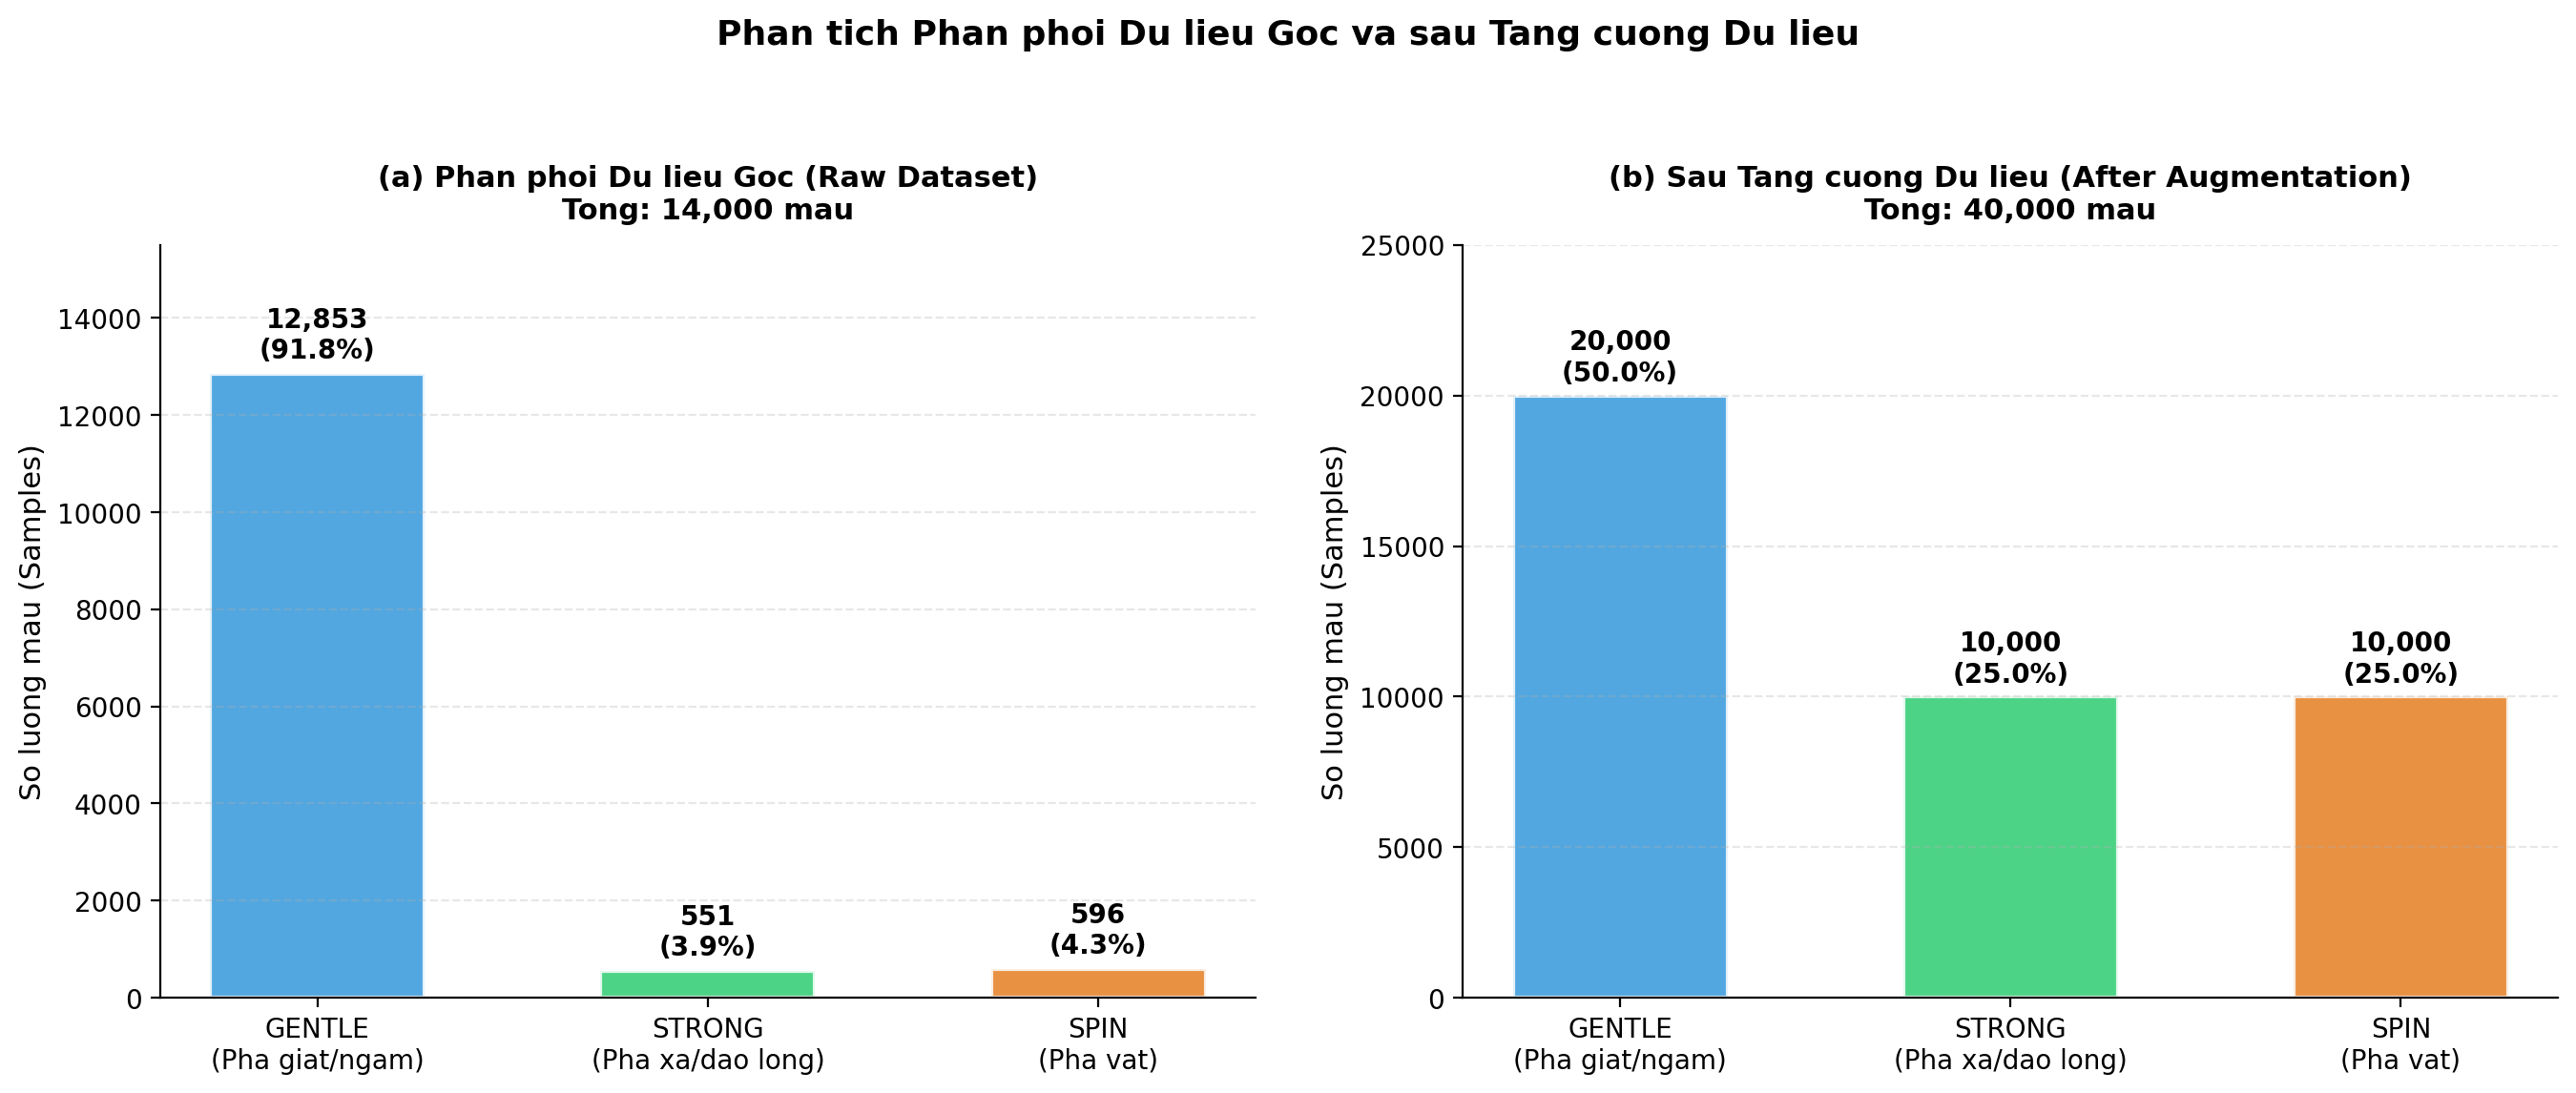
\includegraphics[width=1.0\linewidth]{chap3/image/fig_data_distribution.png}
    \caption[Phân phối dữ liệu trước và sau tăng cường]{Phân phối dữ liệu ba trạng thái trước và sau quá trình tăng cường. Tỷ lệ chênh lệch ban đầu (92:4:4) được cân bằng về mức 2:1:1.}
    \label{fig:data_distribution}
\end{figure}

% ==============================================================================
% DANH MỤC TÀI LIỆU THAM KHẢO TRÍCH DẪN (MỤC 3.1)
% ==============================================================================
% \bibitem{ref_1_8} M. Abdallah et al., "Anomaly Detection and Inter-Sensor Transfer Learning on Smart Manufacturing Datasets," Sensors, vol. 23, no. 1, p. 486, 2023.



\section{Trích xuất đặc trưng và tiền xử lý dữ liệu}

Dữ liệu thô từ các cảm biến ở dạng chuỗi thời gian chứa nhiều nhiễu nền và có số chiều lớn. Bước Trích xuất đặc trưng (Feature Extraction) giữ lại các đặc trưng tiêu biểu nhất về động lực học của máy giặt, tối ưu hóa không gian dữ liệu đầu vào cho mạng nơ-ron trên vi điều khiển.

\subsection{Thiết kế bộ lọc Mel tối ưu cho tín hiệu cơ khí}

Đối với dữ liệu âm thanh, đồ án chuyển đổi sang biểu diễn Năng lượng dải Mel (Mel-Frequency Energy - MFE). Mặc dù phổ Mel được dùng rộng rãi trong xử lý giọng nói, hệ thống tùy chỉnh cấu trúc này cho phân tích tiếng ồn cơ khí:

\begin{itemize}
    \item Tín hiệu âm thanh lấy mẫu ở tần số 8 kHz được phân khung kết hợp cửa sổ Hann để giảm hiện tượng rò rỉ phổ, sau đó áp dụng phép biến đổi Fourier nhanh 512 điểm với bước trượt 256 mẫu.

    \item Thay vì sử dụng 40 hoặc 128 dải Mel như các bài toán phân loại âm thanh tổng quát, hệ thống được tối ưu hóa xuống còn 13 dải lọc tam giác (13 Mel-bins). Các dải lọc tập trung mật độ cao ở vùng tần số thấp và trung — nơi phát ra tiếng ồn vận hành của động cơ và luồng nước — đồng thời giảm độ phân giải ở vùng tần số cao để loại bỏ nhiễu môi trường không mong muốn.

    \item Năng lượng tại mỗi dải Mel được tính theo thang logarit tự nhiên để mô phỏng đặc tính nén dải động của thính giác. Cách tiếp cận này làm nổi bật các dấu hiệu bất thường có biên độ nhỏ vốn dễ bị lấn át bởi nhiễu nền. Kết quả đầu ra là một vector 13 chiều cho mỗi khung âm thanh.
\end{itemize}

\begin{figure}[H]
    \centering
    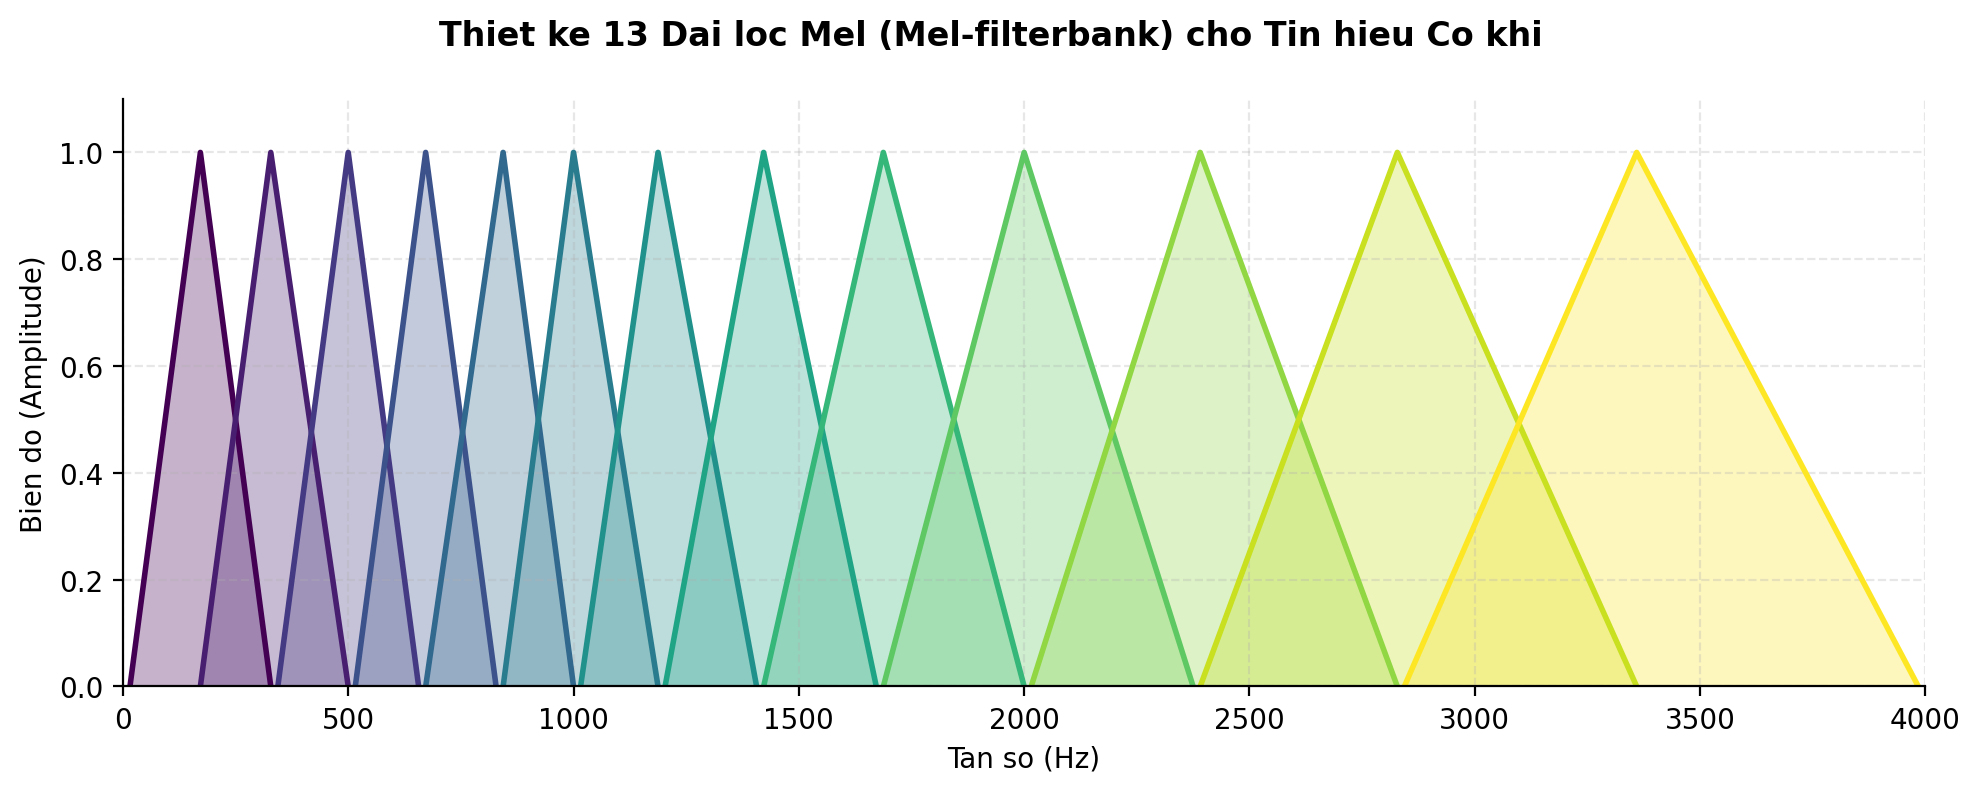
\includegraphics[width=0.9\linewidth]{chap3/image/fig_mel_filterbank.png}
    \caption[Cấu trúc 13 dải lọc Mel]{Trực quan hóa cấu trúc 13 dải lọc Mel tùy chỉnh được sử dụng trong hệ thống. Các bộ lọc hình tam giác được thiết kế phi tuyến, tập trung ở vùng tần số thấp (dưới 1000 Hz) để bóc tách tối đa âm thanh cơ học của máy giặt, đồng thời giảm phân giải ở dải tần cao để hạn chế nhiễu môi trường.}
    \label{fig:mel_filterbank}
\end{figure}

\subsection{Kỹ thuật đồng bộ hóa thuật toán xử lý giữa Python và Firmware C++}

Khi phát triển TinyML, sai lệch biểu diễn (Representation Mismatch) là vấn đề thường gặp. Trong giai đoạn thử nghiệm đầu, mô hình mạng nơ-ron tự mã hóa đạt độ chính xác cao trên Python nhưng sinh ra cảnh báo giả khi triển khai lên vi điều khiển Seeed Studio XIAO ESP32-S3.

Nguyên nhân là sự khác biệt trong tính toán dấu phẩy động: Python sử dụng thư viện \texttt{librosa} với độ chính xác kép (Float64), trong khi firmware C++ thực thi các hàm FFT bằng tập lệnh vector trên kiến trúc Xtensa LX7 chỉ hỗ trợ Float32, kết hợp với mảng lọc tĩnh \texttt{MEL\_FB} tự định nghĩa. Sai số tích lũy qua 13 dải tần đã làm thay đổi phân phối của vector đặc trưng đầu vào so với lúc huấn luyện.

Để khắc phục, đồ án thiết kế lại luồng trích xuất đặc trưng theo cơ chế nhất quán:

\begin{enumerate}
    \item Loại bỏ sự phụ thuộc vào \texttt{librosa}. Mã nguồn Python được viết lại để tính toán FFT và Mel-filterbank bằng các phép toán ma trận NumPy cơ bản, mô phỏng chính xác logic làm tròn số và mảng \texttt{MEL\_FB} của mã nguồn C++.

    \item Áp dụng hệ số nhân tĩnh (Static Scaling Factor) và giới hạn dải năng lượng trong khoảng $[-80, 0]$ dB một cách đồng nhất trên cả hai môi trường.
\end{enumerate}

Phương pháp định hướng firmware (Firmware-Driven Data Pipeline) này đảm bảo nguyên tắc "Train as you deploy", giúp phân phối dữ liệu tại máy chủ huấn luyện và thiết bị biên trùng khớp nhau.

\subsection{Xử lý dữ liệu ngoại lai cho tín hiệu rung động}

Đối với cảm biến gia tốc ADXL345, 6 đặc trưng thống kê được trích xuất bao gồm giá trị hiệu dụng (RMS) và phương sai của ba trục X, Y, Z. Dữ liệu chấn động của máy giặt chứa nhiều ngoại lai (Outliers) mang tính nhất thời, chẳng hạn như tiếng cúc áo va đập vào lồng giặt hoặc sự xô lệch đột ngột của tải trọng.

Nếu áp dụng MinMax Scaling tiêu chuẩn, một gai nhiễu đơn lẻ có thể làm thay đổi toàn bộ dải cực trị, nén 99\% dữ liệu bình thường vào một dải biên độ hẹp và mất khả năng phân biệt các biến động nhỏ. Do đó, đồ án sử dụng kỹ thuật xử lý hỗn hợp (Hybrid Scaling):

\begin{enumerate}
    \item \textbf{Cắt xén ngoại lai (Clipping):} Đối với phương sai trục X và trục Y (nhạy cảm với va đập), thuật toán xác định ngưỡng cắt tại phân vị thứ 99 của tập huấn luyện và giới hạn các giá trị vượt ngưỡng về mức biên này (99th Percentile Clipping). Riêng phương sai trục Z được giữ nguyên dải giá trị ban đầu, vì đây là đặc trưng quyết định để phân loại trạng thái ba trạng thái.

    \item \textbf{Chuẩn hóa (Scaling):} Dữ liệu sau khi qua bộ lọc Clipping được chuẩn hóa bằng RobustScaler. Đồ án mở rộng khoảng phân vị tính toán lên $(10, 90)$ thay vì IQR tiêu chuẩn $(25, 75)$ để bao quát tốt hơn dải động của cảm biến \cite{ref_3_robust_scaler}. Đồng thời, một hệ số bù tối thiểu $0.002$ được cộng thêm vào mẫu số để tránh lỗi chia cho 0 khi máy giặt ở pha tĩnh (GENTLE), đảm bảo tính ổn định số học của hệ thống.
\end{enumerate}

% ==============================================================================
% DANH MỤC TÀI LIỆU THAM KHẢO TRÍCH DẪN (MỤC 3.2)
% ==============================================================================
% \bibitem{ref_3_robust_scaler} P. J. Rousseeuw and A. M. Leroy, "Robust Regression and Outlier Detection," John Wiley & Sons, 2005.


% ==============================================================================
% HẾT MỤC 3.2
% ==============================================================================


% --- Hết chương 3 mục 2 ---

% ============================================================
% Cấu hình huấn luyện và lượng tử hóa mô hình
%
% Tổng hợp quy trình huấn luyện theo mã nguồn training.py
% ============================================================



\section{Cấu hình huấn luyện và lượng tử hóa mô hình}

Sau khi dữ liệu được tiền xử lý và chuẩn hóa về dải $[0, 1]$, bước tiếp theo là xây dựng quy trình huấn luyện và nén mô hình nhằm đáp ứng các giới hạn về bộ nhớ và năng lực tính toán của Seeed Studio XIAO ESP32-S3.

\subsection{Phân chia tập huấn luyện, kiểm định và kiểm thử}

Quá trình huấn luyện được thực hiện riêng cho từng pha vận hành nhằm tránh việc mô hình bị chi phối bởi trạng thái GENTLE vốn chiếm tỷ trọng lớn trong dữ liệu thô. Từ tập \texttt{train\_features\_v6.csv} gồm 14.000 vectơ đặc trưng 19 chiều, dữ liệu được phân hoạch theo phương sai trục Z thành ba tập GENTLE, STRONG và SPIN như đã trình bày ở Mục~\ref{subsec:data_distribution_balance}. Sau đó, mỗi tập trạng thái được tăng cường độc lập trước khi đưa vào mô hình tự mã hóa tương ứng.

Trong mã huấn luyện, tập kiểm định được tách trực tiếp từ dữ liệu sau tăng cường bằng tham số \texttt{validation\_split=0.15}. Như vậy, 85\% dữ liệu tăng cường được dùng để cập nhật trọng số mô hình, còn 15\% được giữ lại để theo dõi sai số kiểm định và kích hoạt cơ chế dừng sớm. Tập kiểm thử cuối cùng không được dùng trong quá trình tối ưu trọng số; các đánh giá định lượng trên tập kiểm thử độc lập và dữ liệu lỗi giả lập được trình bày ở Chương 4.

\begin{table}[H]
    \centering
    \caption{Cách chia dữ liệu huấn luyện và kiểm định theo từng pha vận hành.}
    \label{tab:train_val_split}
    \begin{tabular}{lcccc}
        \hline
        \textbf{Pha} & \textbf{Mẫu gốc} & \textbf{Sau tăng cường} & \textbf{Huấn luyện 85\%} & \textbf{Kiểm định 15\%} \\
        \hline
        GENTLE & 12.853 & 20.000 & 17.000 & 3.000 \\
        STRONG & 551 & 10.000 & 8.500 & 1.500 \\
        SPIN & 596 & 10.000 & 8.500 & 1.500 \\
        \hline
    \end{tabular}
\end{table}

\subsection{Kỹ thuật tăng cường dữ liệu}
Phương pháp học không giám sát yêu cầu tập dữ liệu huấn luyện bao quát được các biến động tự nhiên của môi trường vận hành bình thường. Hệ thống áp dụng các phương pháp tăng cường dữ liệu trực tiếp trên tín hiệu vật lý: Điều chỉnh rung (Vibration Scaling), Dịch chuyển biên độ âm thanh (Audio Volume Shifting) và Rung động từng trục (Per-axis Jittering) (chi tiết tại Mục~\ref{subsec:data_distribution_balance}).

\subsection{Quá trình huấn luyện mô hình số thực (Float32)}

Mô hình đối xứng được thiết kế theo cấu trúc thắt cổ chai sâu (Deep Bottleneck) với số lượng nơ-ron qua các lớp lần lượt là: $19 \rightarrow 128 \rightarrow 64 \rightarrow 32 \rightarrow 64 \rightarrow 128 \rightarrow 19$. Việc mở rộng không gian đặc trưng ở lớp ẩn đầu tiên (từ 19 lên 128 chiều) tạo cấu trúc biểu diễn dư thừa, cung cấp đủ không gian để trích xuất các mối tương quan phi tuyến giữa tín hiệu âm thanh và rung động trước khi nén tại lớp cổ chai 32 chiều.

\begin{itemize}
    \item \textbf{Hàm kích hoạt Sigmoid:} Mặc dù ReLU là hàm kích hoạt phổ biến, kiến trúc này sử dụng Sigmoid cho toàn bộ các lớp ẩn. Sigmoid giới hạn giá trị đầu ra trong khoảng $[0, 1]$, thu hẹp dải động của dữ liệu và giảm sai số khi thực hiện lượng tử hóa về định dạng số nguyên 8-bit (INT8).
    
    \item \textbf{Hàm mất mát có trọng số:} Trong vector đầu vào, 13 đặc trưng âm thanh chiếm ưu thế về số lượng, nhưng 6 đặc trưng rung động lại là chỉ báo vật lý quan trọng nhất để xác định lỗi cơ khí. Đồ án định nghĩa hàm \texttt{weighted\_mae()}, đặt trọng số hệ số 5 cho các sai số thuộc nhóm gia tốc, nhằm ưu tiên tối ưu hóa khả năng tái tạo động hình cơ học của lồng giặt.
    
    \item \textbf{Thuật toán tối ưu và khử nhiễu:} Mô hình sử dụng thuật toán tối ưu Adam \cite{ref_adam} với tốc độ học khởi tạo $0{,}001$ trong giai đoạn huấn luyện số thực. Để tăng tính bền vững, dữ liệu đầu vào được cộng thêm nhiễu Gaussian nhẹ có độ lệch chuẩn $0{,}02$ trong miền đã chuẩn hóa $[0,1]$, trong khi hàm mục tiêu yêu cầu mô hình tái tạo lại tín hiệu sạch. Cách tiếp cận này giúp mô hình học được các đặc trưng cốt lõi và tránh hội tụ về hàm đồng nhất (identity function).
\end{itemize}

\begin{table}[H]
    \centering
    \caption{Cấu hình huấn luyện được sử dụng trong mã nguồn \texttt{training.py}.}
    \label{tab:training_config}
    \begin{tabular}{lcc}
        \hline
        \textbf{Thông số} & \textbf{Tiền huấn luyện Float32} & \textbf{Tinh chỉnh QAT INT8} \\
        \hline
        Thuật toán tối ưu & Adam & Adam \\
        Tốc độ học & $1\times10^{-3}$ & $1\times10^{-4}$ \\
        Số epoch tối đa & 200 & 80 \\
        Batch size & 64 & 64 \\
        Tỷ lệ kiểm định & 15\% & 15\% \\
        Dừng sớm & Patience 20 & Patience 15 \\
        Khôi phục trọng số tốt nhất & Có & Có \\
        \hline
    \end{tabular}
\end{table}


\subsection{Lượng tử hóa nhận thức huấn luyện}

Để triển khai mô hình trên vi điều khiển Seeed Studio XIAO ESP32-S3, kích thước trọng số phải được nén. Thay vì sử dụng lượng tử hóa sau huấn luyện (PTQ), đồ án áp dụng lượng tử hóa nhận thức huấn luyện. Phương pháp này tích hợp các phép toán mô phỏng lượng tử hóa vào quá trình tinh chỉnh (Fine-tuning), giúp mô hình điều chỉnh trọng số để bù cho sai số do giảm độ phân giải số học.

Quá trình huấn luyện được chia thành hai giai đoạn:
\begin{enumerate}
    \item \textbf{Giai đoạn 1 - Tiền huấn luyện:} Mô hình được huấn luyện với định dạng số thực trong tối đa 200 epochs, batch size 64 và cơ chế dừng sớm sau 20 epochs nếu sai số kiểm định không cải thiện. Sai số kiểm định (Val Loss) hội tụ ở mức xấp xỉ \textbf{0,0210} (đối với pha SPIN).
    \item \textbf{Giai đoạn 2 - Tinh chỉnh:} Mô hình sau tiền huấn luyện được bọc bằng lớp lượng tử hóa nhận thức huấn luyện và tiếp tục tối ưu thêm tối đa 80 epochs với tốc độ học $1\times10^{-4}$. Cơ chế dừng sớm được đặt patience 15. Nhờ QAT, sai số kiểm định chỉ tăng không đáng kể lên mức \textbf{0,0225}.
\end{enumerate}
Mức suy giảm hiệu năng dưới 7\% chứng tỏ QAT bảo toàn độ chính xác của mô hình khi chuyển đổi sang môi trường nhúng.

Sau khi huấn luyện, các mô hình được xuất dưới dạng mảng C (Mảng C). Mỗi mô hình đơn lẻ (25.779 tham số) sau lượng tử hóa INT8 có kích thước xấp xỉ \textbf{31,7 KB}. Tổng dung lượng cho tổ hợp 3 mô hình (hỗn hợp Ba trạng thái) chỉ chiếm \textbf{95,3 KB}, giảm 4 lần so với mô hình Float32, cho phép triển khai thuật toán chuyển đổi trạng thái mà không tăng áp lực lên bộ nhớ Flash.

\subsection{Xác định ngưỡng cảnh báo dựa trên quy tắc $3\sigma$}
Ngưỡng phát hiện dị thường ($\tau$) cho từng pha được thiết lập từ phân phối sai số tái tạo của tập dữ liệu bình thường, tuân theo quy tắc ba sigma ($3\sigma$):
\begin{equation}
    \tau = \mu_{MAE} + 3 \cdot \sigma_{MAE}
\end{equation}

Lựa chọn hệ số $k=3$ thay vì các ngưỡng tối ưu theo chỉ số Youden's J phản ánh yêu cầu thực tiễn: cảnh báo giả (False Positive) gây ảnh hưởng tiêu cực đến người dùng nghiêm trọng hơn phản hồi chậm đối với một số dị thường nhỏ (False Negative). Ngưỡng $3\sigma$ cung cấp dải biên an toàn lớn, đảm bảo độ chính xác (Precision) cao trước khi phát tín hiệu hỏng hóc.

Các ngưỡng cố định được xác lập tương ứng: GENTLE ($0{,}1241$), STRONG ($0{,}0968$), và SPIN ($0{,}0672$).


% ============================================================
% MỤC: XUẤT THÔNG SỐ CẤU HÌNH VÀ THAM SỐ MÔ HÌNH CHO VI ĐIỀU KHIỂN
% ============================================================


\subsection{Đánh giá cấu hình và hiệu năng tài nguyên}

Kiến trúc mạng nơ-ron sử dụng toàn bộ hàm kích hoạt Sigmoid để giới hạn dữ liệu trong dải $[0, 1]$, ngăn ngừa các lỗi tràn bộ đệm khi vi điều khiển thực thi các phép toán nhân ma trận INT8.

\begin{table}[H]
    \centering
    \caption[Chi tiết tham số mạng tự mã hóa]{Chi tiết cấu trúc các lớp và số lượng tham số của một mô hình tự mã hóa thành phần.}
    \label{tab:ae_params}
    \begin{tabular}{clcc}
        \hline
        \textbf{STT} & \textbf{Lớp} & \textbf{Kích thước} & \textbf{Tham số} \\
        \hline
        1 & Đầu vào      & $19$    & ---    \\
        2 & Dense (Encoder-1)    & $128$   & $2.560$ \\
        3 & Dense (Encoder-2)    & $64$    & $8.256$ \\
        4 & Dense (lớp thắt cổ chai)   & $32$    & $2.080$ \\
        5 & Dense (Decoder-1)    & $64$    & $2.112$ \\
        6 & Dense (Decoder-2)    & $128$   & $8.320$ \\
        7 & Đầu ra      & $19$    & $2.451$ \\
        \hline
        \multicolumn{3}{r}{\textbf{Tổng cộng:}} & \textbf{25.779} \\
        \hline
    \end{tabular}
\end{table}

Kích thước tối ưu này (95,3 KB cho 3 mô hình) giúp thời gian tính toán suy luận trên lõi Xtensa LX7 của vi điều khiển Seeed Studio XIAO ESP32-S3 đạt mức khoảng 6,4 ms (Bảng~\ref{tab:latency_stats}), chỉ chiếm 0,64\% quỹ thời gian của một chu kỳ lấy mẫu 1 Hz, duy trì tần số lấy mẫu tốc độ cao mà không làm chậm các tiến trình khác trong hệ điều hành FreeRTOS.


% --- Kết thúc chương 3 mục 4 ---

\section{Kiểm chứng tính nhất quán của hệ thống}
\label{sec:kiem_chung_nhat_quan}

Khi triển khai các hệ thống học máy tại biên, hiện tượng không khớp triển khai — sự sai lệch kết quả suy luận giữa môi trường huấn luyện (Python/TensorFlow) và môi trường thực thi (C++/TFLite Micro) — là vấn đề phổ biến. Phần này trình bày các phương pháp kiểm chứng tính nhất quán của toàn bộ đường ống xử lý, từ tiền xử lý đến suy luận cuối cùng.

\subsection{Đối chiếu phân phối đặc trưng giữa môi trường giả lập và phần cứng}

Trong giai đoạn đầu phát triển, mô hình đạt độ chính xác cao trên tập kiểm thử nhưng sinh ra nhiều cảnh báo giả khi nạp xuống vi điều khiển Seeed Studio XIAO ESP32-S3. Nguyên nhân bắt nguồn từ sự bất đồng bộ trong thuật toán trích xuất đặc trưng âm thanh giữa hai môi trường.

Kịch bản Python ban đầu sử dụng thư viện \texttt{librosa} với độ chính xác kép (Float64), trong khi firmware C++ sử dụng thư viện \texttt{esp-dsp} với Float32. Sự khác biệt về thư viện và độ chính xác số học này làm thay đổi phân phối dữ liệu đầu vào.

Để khắc phục, hệ thống thực hiện đồng bộ hóa thuật toán:
\begin{itemize}
    \item \textbf{Đồng nhất tham số DSP:} Loại bỏ sự phụ thuộc vào \texttt{librosa}. Mã nguồn Python được viết lại bằng NumPy để mô phỏng logic tính toán của vi điều khiển. Cấu hình cố định: cửa sổ Hann, FFT 512 điểm và bước trượt 256 mẫu. Với bộ đệm 1 giây ở tần số lấy mẫu 8 kHz, số khung hợp lệ được tính theo $\lfloor(8000-512)/256\rfloor + 1 = 30$, đúng với cấu hình firmware.
    \item \textbf{Cố định dải động:} Năng lượng tín hiệu qua bộ lọc Mel được giới hạn và ánh xạ về khoảng $[-80, 0]$ dB trên cả hai môi trường. Xác thực thông qua đồ thị phân phối xác minh ma trận đặc trưng từ Python và dữ liệu từ bộ nhớ của vi điều khiển Seeed Studio XIAO ESP32-S3 trùng khớp ở cấp độ bit.
\end{itemize}

\begin{figure}[H]
    \centering
    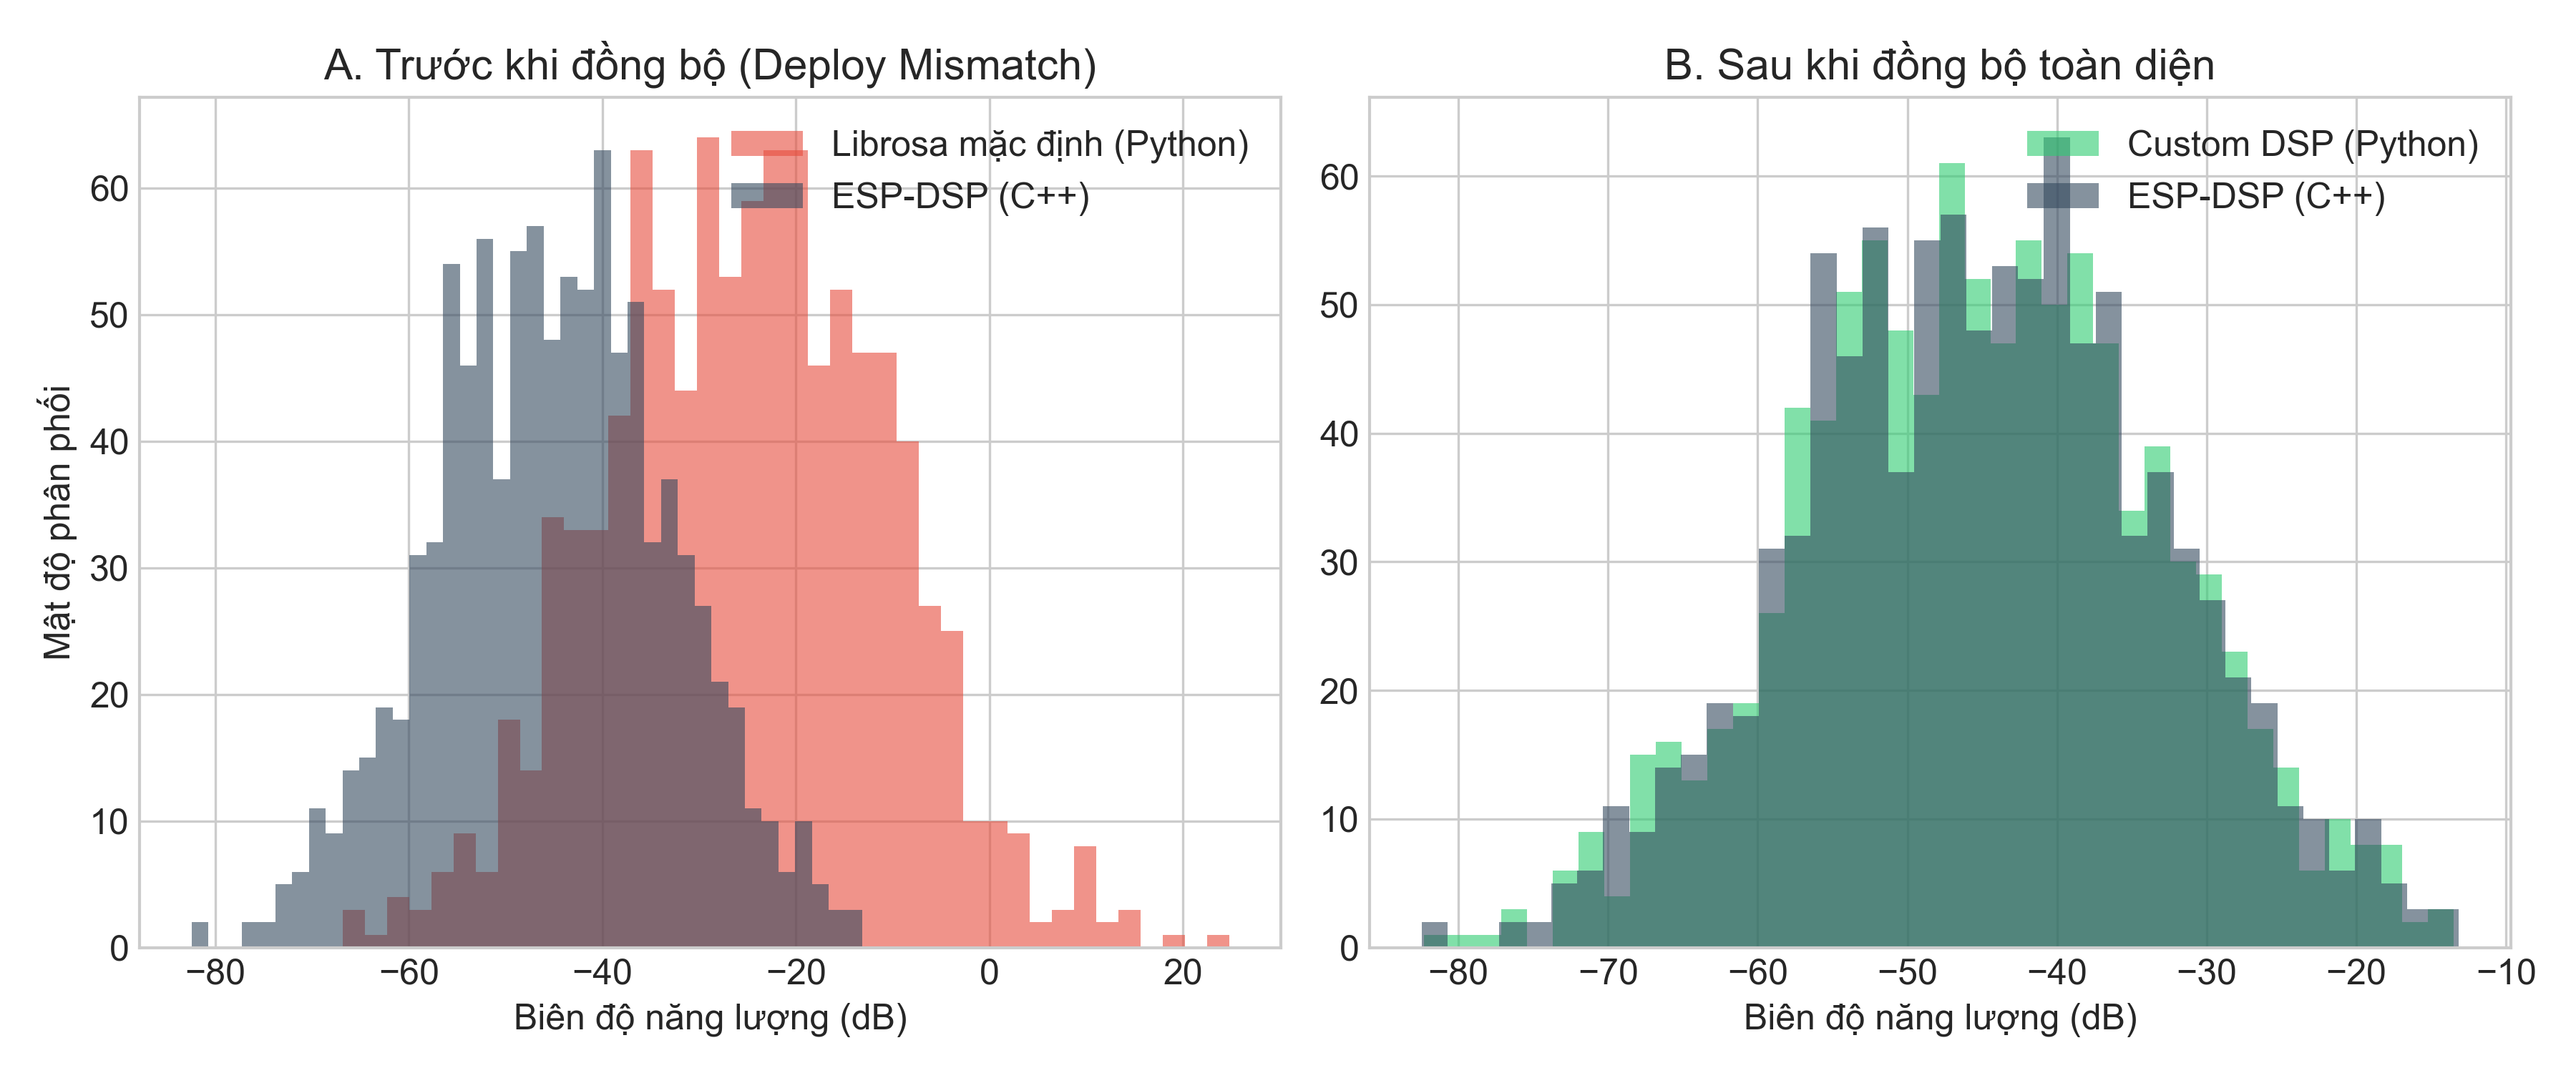
\includegraphics[width=0.9\linewidth]{chap4/image/dsp_histogram_match.png}
    \caption[Đối chiếu phân phối năng lượng âm thanh]{Đối chiếu phân phối năng lượng phổ âm thanh trước và sau khi đồng bộ thuật toán DSP giữa Python và C++.}
    \label{fig:dsp_mismatch}
\end{figure}

\subsection{Xác thực tính toàn vẹn của đồ thị suy luận}

Sau khi xuất mô hình dưới dạng mảng byte, xác thực tính toàn vẹn bộ nhớ khi nạp qua TensorFlow Lite Micro là bước quan trọng. Hệ thống sử dụng xác thực chéo ở cấp độ tensor:

\begin{enumerate}
    \item \textbf{Trích xuất vector kiểm thử:} 100 vector đặc trưng ngẫu nhiên từ Python được sử dụng làm dữ liệu nền kiểm chứng.
    \item \textbf{Quản lý vùng nhớ an toàn:} Để tránh lỗi phân mảnh và tràn bộ nhớ cấp phát động, mảng bộ nhớ làm việc trung gian (\texttt{tensor\_arena}) được cấp phát tĩnh. Kích thước vùng nhớ được tính toán tối ưu với cấu trúc mạng và đặt tại phân vùng SRAM nội bộ để tăng tốc độ truy xuất. Điều này cho phép thiết bị chuyển đổi linh hoạt giữa 3 mô hình (GENTLE, STRONG, SPIN) trên cùng một vùng nhớ trung gian mà không cần cấp phát lại bộ nhớ.
    \item \textbf{Suy luận song song và đối chiếu:} Một vector đầu vào được đưa qua mô hình Float32 trên máy tính và mô hình INT8 trên vi điều khiển. Đầu ra \texttt{int8\_t} từ vi điều khiển Seeed Studio XIAO ESP32-S3 được gửi qua cổng Serial để so sánh từng phần tử với mảng đầu ra trên máy chủ.
\end{enumerate}

Bộ thông dịch TFLM thực thi đồ thị mạng ổn định, không ghi nhận tràn vùng nhớ đệm hay lỗi sai số vượt ngưỡng trong quá trình lượng tử hóa.


\chapter{TRIỂN KHAI VÀ ĐÁNH GIÁ KẾT QUẢ}


\label{chuong_4}

\section{Triển khai phần mềm trên vi điều khiển Seeed Studio XIAO ESP32-S3}

Chuyển đổi từ mô hình học máy lý thuyết sang hệ thống nhúng ổn định yêu cầu tối ưu hóa sâu về mặt thực thi. Phần này trình bày các giải pháp kỹ thuật để triển khai kiến trúc mạng nơ-ron tự mã hóa Ba trạng thái trên phần cứng tài nguyên hạn chế.

\subsection{Chiến lược quản lý bộ nhớ cho hệ thống đa mô hình}

Hệ thống sử dụng ba mô hình mạng nơ-ron tự mã hóa độc lập cho ba trạng thái (GENTLE, STRONG, SPIN), với tổng dung lượng 95,3~KB. Trong kiến trúc TensorFlow Lite Micro, quản lý bộ nhớ được chia thành hai vùng riêng:
\begin{itemize}
    \item Vùng nhớ trọng số tĩnh: Mảng C chứa cấu trúc và trọng số mô hình từ \texttt{model\_data.h} được khai báo với từ khóa \texttt{const}, buộc trình biên dịch lưu trữ trên bộ nhớ Flash. Vi điều khiển truy xuất trực tiếp các trọng số thông qua cơ chế ánh xạ bộ nhớ đệm của ESP32-S3 mà không cần sao chép vào RAM.
    \item Vùng nhớ nội suy: Xử lý dữ liệu kích hoạt giữa các lớp nơ-ron theo thời gian thực bằng vùng đệm tensor. Do lớp thắt cổ chai 32-chiều nhỏ gọn, vùng đệm tensor chỉ chiếm vài kilobyte trên SRAM nội bộ siêu tốc.
\end{itemize}
Chiến lược này loại bỏ độ trễ nạp mô hình, đảm bảo hệ thống không mất mẫu dữ liệu trong các pha chuyển tiếp của máy giặt.

\subsection{Thực thi tiền xử lý tín hiệu trực tiếp trên Firmware}

Để không gian suy luận thực tế trùng khớp với không gian huấn luyện, vi điều khiển thực thi trực tiếp các thuật toán xử lý tín hiệu số bằng các hàm tối ưu hóa phần cứng.

\begin{itemize}
    \item Chuẩn hóa phổ âm thanh: Sau FFT 512-điểm và bộ lọc Mel, năng lượng phổ được tính dưới dạng Log-dB. Thư viện \texttt{esp-dsp} gia tốc các phép toán logarit bằng tập lệnh vector phần cứng. Các giá trị biên độ sau đó được ánh xạ tuyến tính về dải $[0, 1]$ dựa trên hệ số Min ($-80{,}0$) và Scale ($80{,}0$) từ quá trình huấn luyện.
    \item Chuẩn hóa rung động: Firmware thực thi công thức: $z = \frac{x - \text{median}}{\text{IQR}}$. Toàn bộ 36 tham số median và IQR cho 3 pha đã được tính sẵn từ Python và lưu dưới dạng hằng số \texttt{const float}. Để tránh chia cho không khi máy ở trạng thái tĩnh, hằng số epsilon $\epsilon = 0{,}002$ được cộng vào mẫu số.
\end{itemize}

\subsection{Tính toán sai số tái tạo trên miền lượng tử hóa (INT8-domain)}

Hệ thống thực hiện tính toán sai số tái tạo trực tiếp trên miền số nguyên thay vì miền số thực. Vì mô hình đầu ra và dữ liệu đầu vào đều được lượng tử hóa sang INT8, phép tính MAE được thực thi theo công thức:
\begin{equation}
    \text{MAE}_{int8} = \frac{1}{N} \sum_{i=1}^{N} \left| x_{quantized}^{(i)} - \hat{x}_{quantized}^{(i)} \right|
\end{equation}

Các phép trừ và giá trị tuyệt đối trên kiểu \texttt{int8\_t} tiêu tốn ít chu kỳ máy và tương thích tối ưu với tập lệnh SIMD của ESP32-S3 \cite{ref_1_15}. Sau khi có tổng $\text{MAE}_{int8}$, hệ thống thực hiện một phép nhân duy nhất với hệ số tỉ lệ để giải lượng tử hóa kết quả về Float32 và so sánh với ngưỡng cảnh báo. Phương pháp này giảm chu kỳ CPU hơn 4 lần so với giải lượng tử hóa từng phần tử đầu ra, góp phần duy trì tổng thời gian suy luận ở mức chỉ vài mili-giây.

\subsection{Cơ chế lọc trễ thời gian}
\label{subsec:temporal_debounce}

Để loại bỏ cảnh báo giả do nhiễu tức thời, hệ thống triển khai bộ lọc cửa sổ trượt kết hợp cơ chế trễ trong logic ra quyết định. Thay vì kích hoạt cảnh báo ngay khi một mẫu vượt ngưỡng, hệ thống quan sát chuỗi trạng thái của 10 cửa sổ liên tiếp (tương đương khoảng 10 giây vận hành):

\begin{itemize}
    \item \textbf{Điều kiện kích hoạt:} Trạng thái cảnh báo (ALARM) chỉ được xác lập khi có ít nhất 5 trên 10 mẫu gần nhất vượt ngưỡng $\tau$.
    \item \textbf{Cơ chế duy trì và thoát:} Khi đã ở trong trạng thái cảnh báo, yêu cầu độ tin cậy cao hơn để phục hồi. Cảnh báo chỉ được gỡ bỏ khi có ít nhất 9 trên 10 mẫu gần nhất trở về mức an toàn (tức là chỉ cho phép tối đa 1 mẫu vượt ngưỡng).
\end{itemize}

Cơ chế bất đối xứng này ngăn dao động trạng thái (chống nhiễu "chập chờn") tại vùng biên của ngưỡng cắt, đồng thời ưu tiên an toàn thiết bị bằng cách duy trì cảnh báo cho đến khi sự cố được khắc phục ổn định.

\begin{figure}[H]
    \centering
    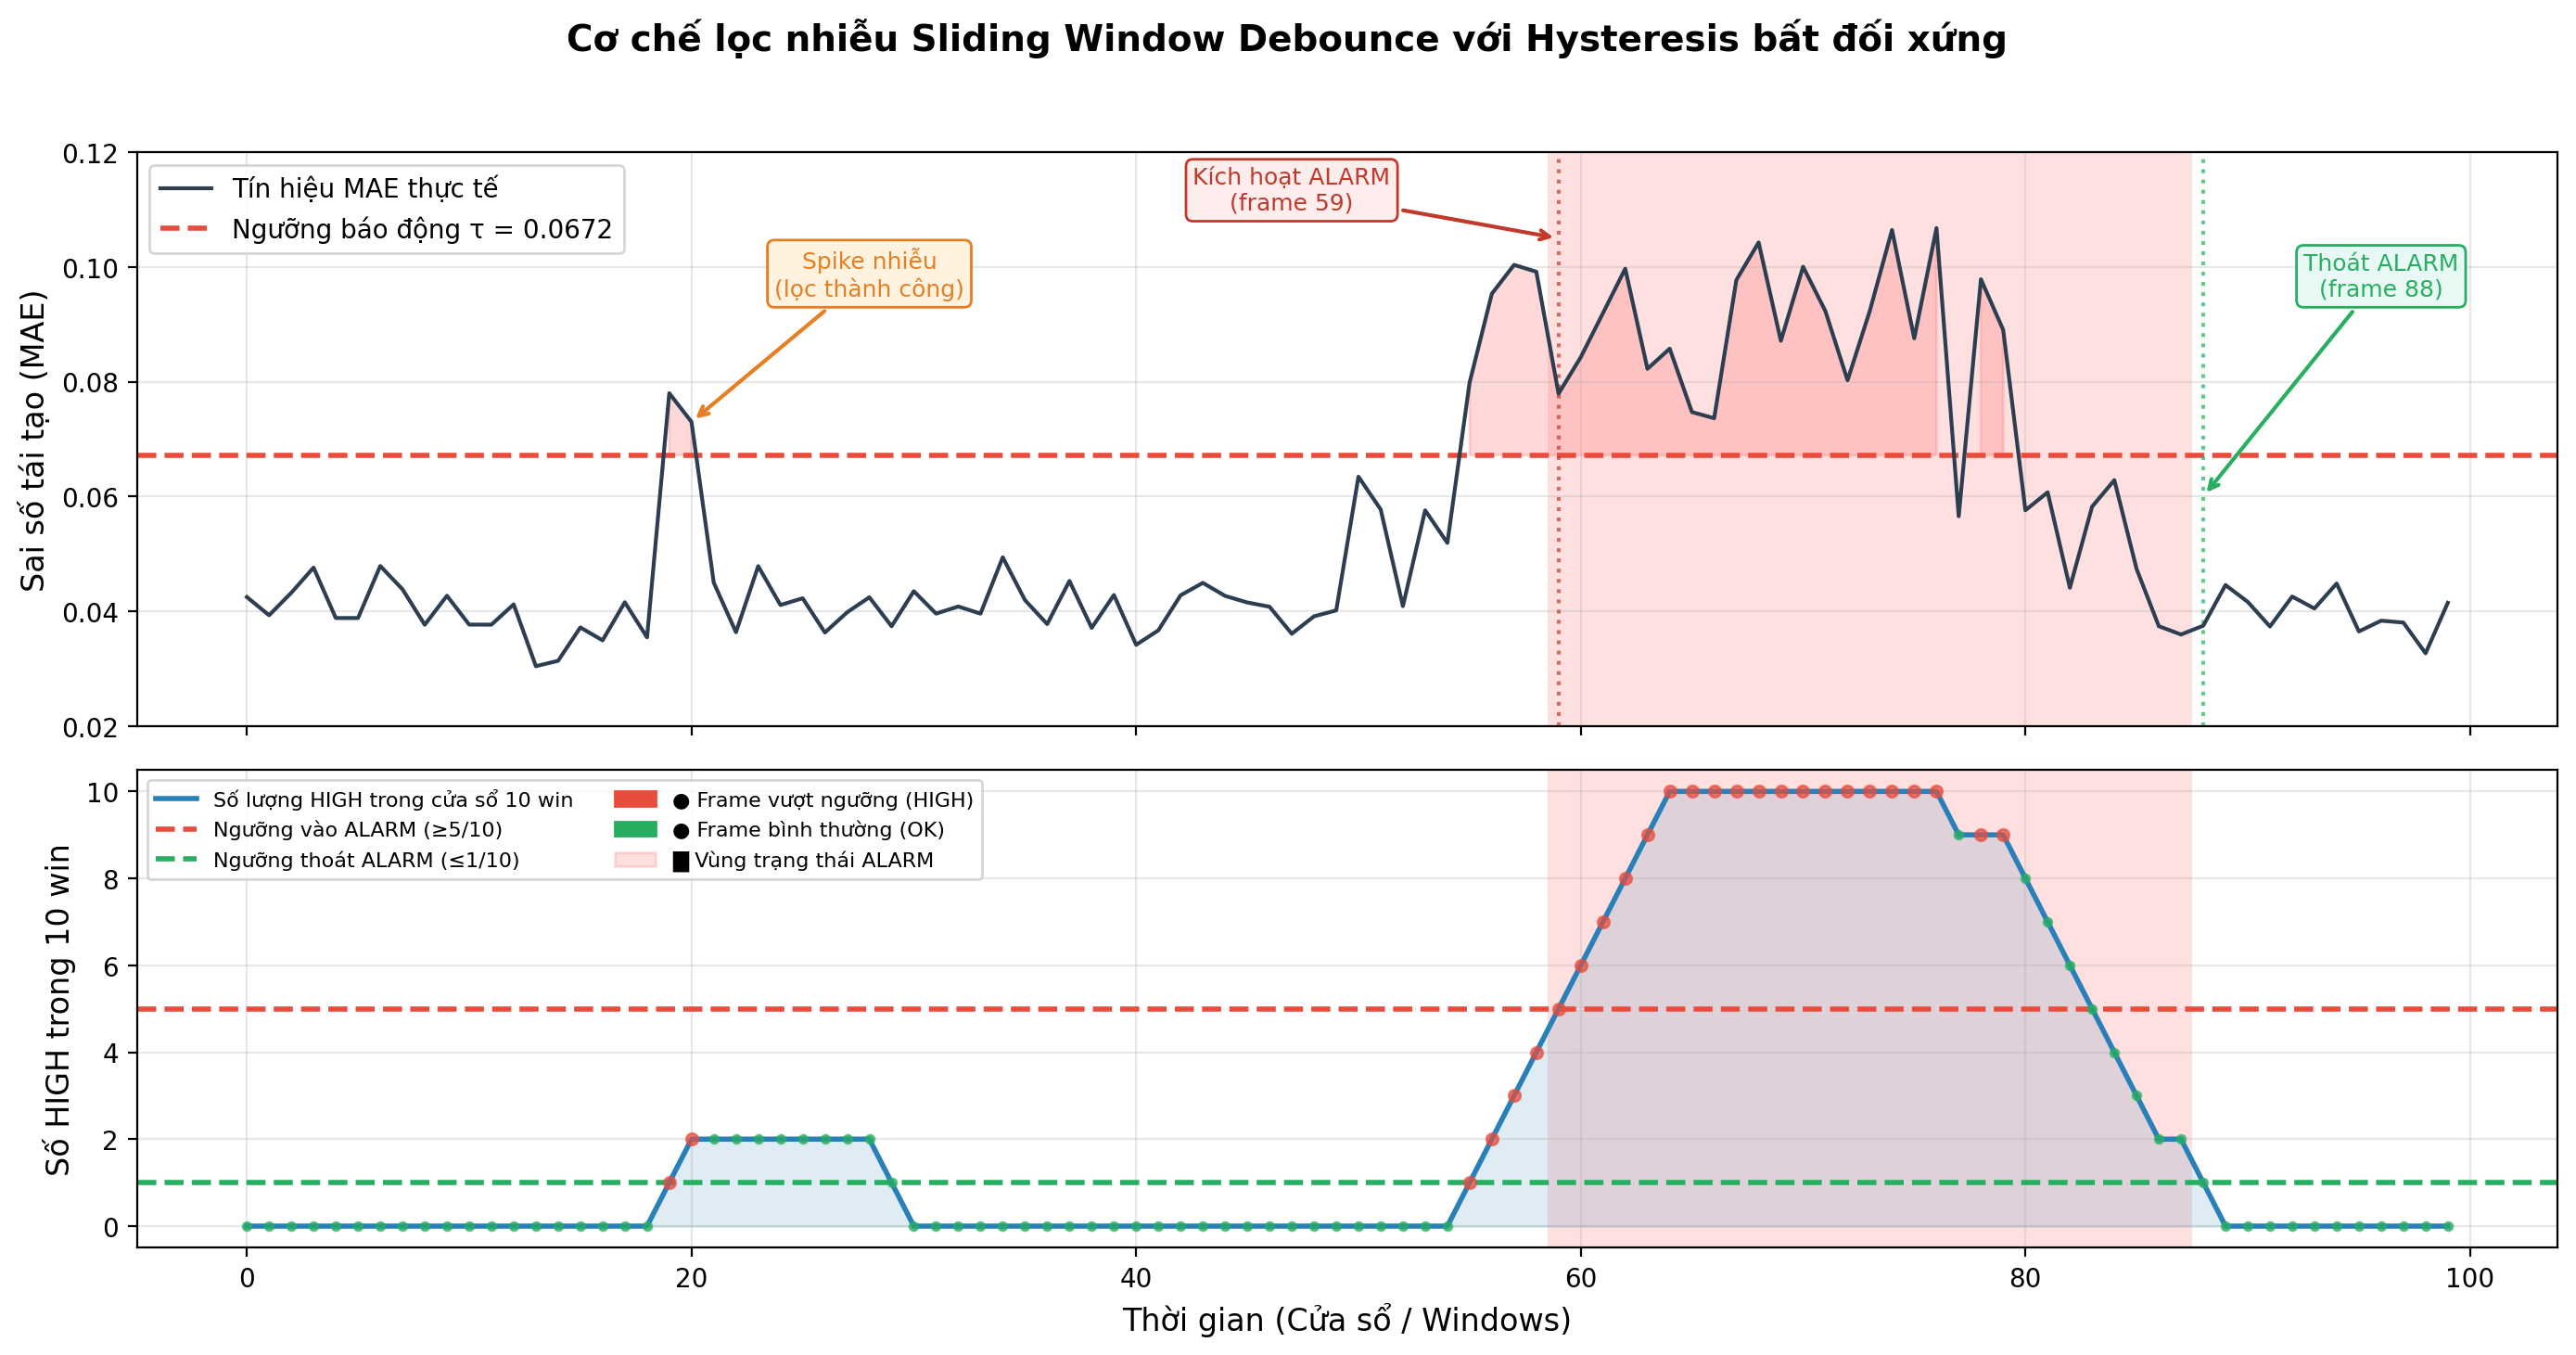
\includegraphics[width=0.95\linewidth]{chap4/image/debounce_sliding_window.png}
    \caption[Cơ chế lọc nhiễu bằng cửa sổ trượt]{Mô phỏng cơ chế cửa sổ trượt kết hợp trễ bất đối xứng: kích hoạt cảnh báo khi $\geq 5/10$ mẫu vượt ngưỡng, phục hồi khi $\leq 1/10$ mẫu vượt ngưỡng. Xung nhiễu đơn lẻ (frame 19--21) được lọc hoàn toàn nhờ cơ chế biểu quyết đa số.}
    \label{fig:debounce_logic}
\end{figure}

Kỹ thuật lọc trễ phần mềm này hoạt động như bộ lọc thông thấp cho logic quyết định, loại bỏ các đỉnh nhiễu ngẫu nhiên và giúp hệ thống đạt độ tin cậy cực cao (F1-Score $> 0{,}98$) trong các bài kiểm tra thực địa dài hạn.





\section{Đánh giá hiệu năng hệ thống nhúng}

Triển khai học máy tại biên (\textit{TinyML}) vào sản xuất công nghiệp không chỉ đánh giá dựa trên độ chính xác thuật toán mà còn phụ thuộc vào hiệu năng thực thi trên phần cứng giới hạn. Độ trễ, mức tiêu thụ bộ nhớ và độ ổn định của hệ điều hành thời gian thực (RTOS) là tiêu chí đánh giá tính khả thi của hệ thống \cite{ref_mlperf_tiny}.

\subsection{Phân tích độ trễ suy luận}

Độ trễ suy luận là thời gian từ khi vi điều khiển hoàn tất trích xuất đặc trưng đầu vào (vectơ 19 chiều) cho đến khi đưa ra sai số tái tạo MAE và nhãn phân loại. Duy trì độ trễ suy luận thấp giúp hệ thống phản ứng tức thời với các sự cố cơ khí đột ngột trước khi gây thiệt hại vật lý.

Nhờ lượng tử hóa nhận thức huấn luyện chuyển đổi trọng số sang INT8, hệ thống tối ưu hóa khối lượng tính toán. Bên cạnh đó, Seeed Studio XIAO ESP32-S3 sở hữu kiến trúc lõi kép Xtensa® LX7 tích hợp tập lệnh vector SIMD chuyên dụng cho trí tuệ nhân tạo, thực thi song song các phép toán nhân-tích lũy (MAC) trên mảng dữ liệu \cite{ref_1_15, ref_1_7}.

Để đo đạc chính xác, hệ thống thực hiện đánh giá hiệu năng tự động với N=1\,000 lần suy luận trên từng mô hình, sử dụng hàm \texttt{esp\_timer\_get\_time()} đo trực tiếp thời gian thực thi của hàm \texttt{Invoke()} trong TensorFlow Lite Micro. Kết quả cho thấy thời gian suy luận trung bình tổng hợp đạt \textbf{6,44 ms} (Bảng~\ref{tab:latency_stats}).

\begin{table}[H]
\centering
\caption[Thống kê độ trễ suy luận]{Thống kê độ trễ suy luận trên vi điều khiển Seeed Studio XIAO ESP32-S3 (N=1\,000 mẫu mỗi mô hình, tổng cộng 3\,000 phép đo)}
\label{tab:latency_stats}
\begin{tabular}{|l|c|c|c|c|c|c|}
\hline
\textbf{Mô hình} & \textbf{Mean ($\mu s$)} & \textbf{Std} & \textbf{Min} & \textbf{Max} & \textbf{P95} & \textbf{P99} \\ \hline
GENTLE & 6.411 & 71,9 & 6.274 & 6.536 & 6.516 & 6.526 \\ \hline
STRONG & 6.512 & 21,0 & 6.449 & 6.552 & 6.543 & 6.551 \\ \hline
SPIN   & 6.393 & 20,3 & 6.344 & 6.438 & 6.427 & 6.429 \\ \hline
\rowcolor[HTML]{EFEFEF}
\textbf{Tổng hợp} & \textbf{6.439} & \textbf{68,8} & \textbf{6.274} & \textbf{6.552} & \textbf{6.535} & \textbf{6.545} \\ \hline
\end{tabular}
\end{table}

\begin{figure}[H]
    \centering
    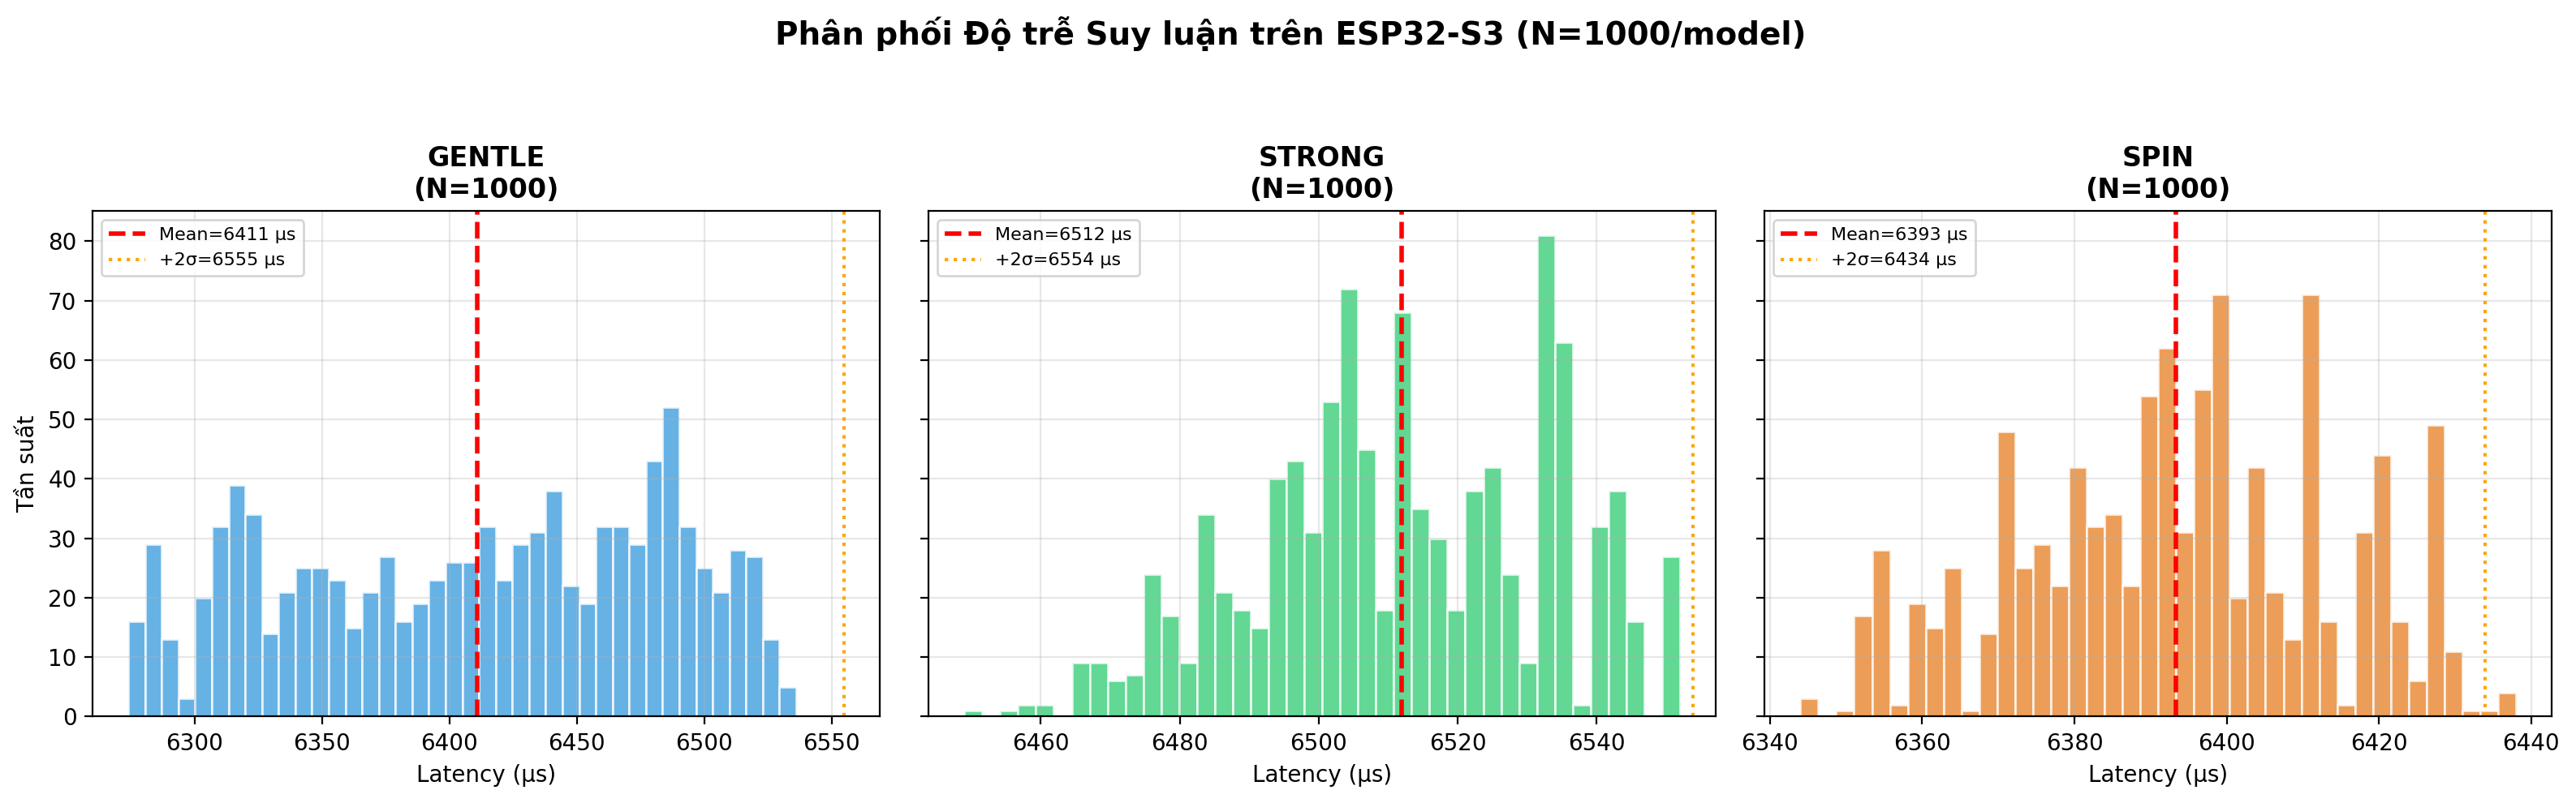
\includegraphics[width=0.95\linewidth]{chap4/image/latency_histogram.png}
    \caption[Phân phối độ trễ suy luận]{Biểu đồ phân phối thực nghiệm của độ trễ suy luận trên vi điều khiển Seeed Studio XIAO ESP32-S3 cho 3 mô hình ba trạng thái. Mỗi mô hình được đo 1\,000 lần suy luận liên tiếp. Độ trễ tập trung ổn định quanh 6,4 ms với độ lệch chuẩn thấp ($< 72 \mu s$).}
    \label{fig:latency_histogram}
\end{figure}

\begin{itemize}
    \item Đánh giá đáp ứng thời gian thực: Với tần số lấy mẫu đặc trưng 1 Hz (chu kỳ 1\,000 ms), thời gian suy luận 6,4 ms chỉ chiếm $0{,}64\%$ quỹ thời gian CPU, dư dả cho các tác vụ khác.
    \item Dư địa tài nguyên: Tác vụ Trí tuệ nhân tạo (AI) hoàn thành trong vài mili-giây, cho phép lõi CPU số 1 nhường tài nguyên cho các tác vụ giao tiếp mạng (MQTT, TLS/SSL) mà không gây nghẽn cổ chai.
    \item Biến động thời gian suy luận: Mô hình GENTLE ghi nhận độ lệch chuẩn cao hơn so với hai mô hình còn lại. Điều này xuất phát từ việc vùng đệm tensor được cấp phát trên PSRAM ngoại vi; các hiện tượng trượt bộ nhớ đệm ngẫu nhiên của vi điều khiển Seeed Studio XIAO ESP32-S3 khi truy xuất dữ liệu qua bus SPI làm tăng nhẹ thời gian của một số chu kỳ. Tuy nhiên, mức chênh lệch này vẫn nằm trong ngưỡng chấp nhận được của hệ thống.
\end{itemize}

\subsection{Đánh giá mức sử dụng tài nguyên bộ nhớ và độ ổn định hệ thống}

Rào cản chính khi đưa các mô hình Học sâu vào vùng biên là dung lượng bộ nhớ tĩnh (Flash) và động (SRAM) eo hẹp \cite{ref_1_7, ref_1_4}.

\textbf{Chiếm dụng bộ nhớ Flash và số lượng tham số:} \\
Hệ thống tối ưu hóa kiến trúc đối xứng với Lớp thắt cổ chai 32 chiều và lượng tử hóa INT8 triệt để. Toàn bộ 3 mô hình (GENTLE, STRONG, SPIN) sau lượng tử hóa INT8 có tổng dung lượng chỉ \textbf{95,3 KB}. Khi tích hợp vào firmware hoàn chỉnh (mã điều khiển, FreeRTOS, TensorFlow Lite for Microcontrollers, thư viện MQTT/TLS, WiFi stack và các driver I2S/I2C), tổng dung lượng Flash được ghi nhận qua kết quả biên dịch thực tế là \textbf{1.254.517 bytes} (xấp xỉ \textbf{1,20 MB}), chiếm \textbf{37\%} không gian chương trình (Hình~\ref{fig:flash_usage}).

\begin{figure}[H]
    \centering
    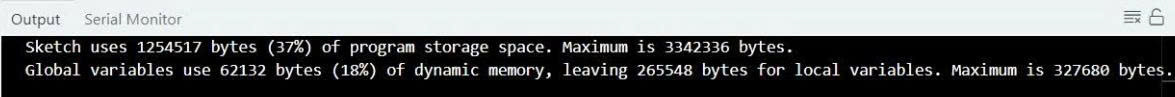
\includegraphics[width=0.85\linewidth]{chap4/image/flash_usage_proof.png}
    \caption[Kết quả biên dịch firmware]{Kết quả biên dịch firmware v11 trên Arduino IDE 2.3.5, xác nhận mức chiếm dụng bộ nhớ Flash (37\%) và SRAM (18\%) thực tế trên vi điều khiển Seeed Studio XIAO ESP32-S3.}
    \label{fig:flash_usage}
\end{figure}

\textbf{Quản lý bộ nhớ động (SRAM/PSRAM):} \\
TensorFlow Lite Micro đòi hỏi vùng nhớ đệm để lưu trữ các tensor trung gian. Nhờ kiến trúc gọn nhẹ, tổng không gian nhớ mà các mô hình yêu cầu rất thấp. Bộ nhớ động (Global Variables) chiếm \textbf{62.132 bytes (18\%)} trên tổng 327.680 bytes SRAM, để dư 265.548 bytes cho các tác vụ thời gian thực. Hệ thống quy hoạch bộ nhớ trên kiến trúc lõi kép Seeed Studio XIAO ESP32-S3:
\begin{enumerate}
    \item Tận dụng SRAM nội bộ (512 KB) cho các bộ đệm DMA tốc độ cao của cảm biến âm thanh và rung động để tránh mất mẫu.
    \item Vùng nhớ (3 × 40 KB) được cấp phát trên PSRAM 8 MB thông qua hàm \texttt{heap\_caps\_aligned\_alloc()}, đảm bảo dư dả tài nguyên cho các tác vụ giao tiếp mạng mà không gây xung đột hay Tràn ngăn xếp.
    \item Hệ thống có thể duy trì hoạt động liên tục trong nhiều chu kỳ giặt mà không xảy ra Rò rỉ bộ nhớ hay Watchdog Reset.
\end{enumerate}

Độ ổn định hệ thống trong thử nghiệm thực địa: \\
Hệ thống được đánh giá qua các bài kiểm tra thực địa kéo dài nhiều chu kỳ hoạt động đầy đủ của máy giặt. Nhờ kiến trúc FreeRTOS đa nhiệm:
\begin{itemize}
    \item Tác vụ thu thập cảm biến trên lõi số 0 và tác vụ suy luận Trí tuệ nhân tạo trên lõi số 1 hoạt động độc lập thông qua Nhóm sự kiện và Hàng đợi.
    \item Tình trạng tác vụ không được cấp đủ thời gian CPU và xung đột tài nguyên được ngăn chặn nhờ gán mức độ ưu tiên (ví dụ: ngắt I2C đo rung động được cấp mức ưu tiên 15 - cao nhất để đảm bảo thời gian thực).
\end{itemize}
Trong các thử nghiệm dài hạn, hệ thống không ghi nhận Rò rỉ bộ nhớ hay Watchdog Reset. Dữ liệu đo xa được duy trì ổn định ở tần suất 1,0 Hz, đảm bảo luồng dữ liệu mượt mà cho cơ chế lọc nhiễu cửa sổ thời gian và kích hoạt cảnh báo tức thời trên ứng dụng di động.

\section{Đánh giá khả năng phát hiện bất thường}
\label{sec:danh_gia_bat_thuong}

Hệ thống học không giám sát nhằm nhận diện các mẫu dữ liệu chệch hướng so với phân phối chuẩn mà không cần gán nhãn trước \cite{ref_1_6}. Để xác thực năng lực này, đánh giá được tiến hành thông qua giả lập các kịch bản lỗi vật lý và phân tích sai số tái tạo trên mô hình TFLite thực tế.

\subsection{Thiết lập kịch bản kiểm thử với giả lập lỗi (Anomaly Injection)}

Hệ thống giả lập các lỗi vật lý trực tiếp trên đối tượng nghiên cứu để tạo ra các điểm bất thường có kiểm soát, tương tự các hư hỏng thường gặp:

\begin{itemize}
    \item \textbf{Mất cân bằng tải trọng (Load Imbalance):} Mô phỏng lệch lồng giặt bằng cách bố trí vật nặng dồn về một phía. Thử nghiệm này buộc hệ thống xử lý các biên độ gia tốc văng lớn bất thường, đặc biệt trong pha SPIN.
    \item \textbf{Biến động âm thanh:} Tạo tiếng ồn ma sát kim loại hoặc va đập nhân tạo để kiểm chứng độ nhạy của bộ lọc Mel 13 dải trước các dấu hiệu hỏng hóc vòng bi hoặc động cơ.
    \item \textbf{Trường hợp biên:} Áp dụng dịch chuyển biên độ và nhiễu biến thiên để kiểm chứng độ bền bỉ của mô hình trước các nhiễu nền ngẫu nhiên trong môi trường dân dụng.
\end{itemize}

\subsection{Phân tích phân phối sai số tái tạo}

Mô hình được kiểm chứng trên \textit{tập dữ liệu v6} — tập kiểm thử độc lập thu thập từ các phiên vận hành tách biệt hoàn toàn với dữ liệu huấn luyện, đảm bảo khả năng tổng quát hóa trước điều kiện môi trường thực tế. Phân tích biểu đồ MAE (Hình~\ref{fig:mae_sep_all}) cho thấy phân tách trạng thái rõ rệt:

\begin{itemize}
    \item \textbf{Pha GENTLE ($n=12.853$):} Mặc dù có cường độ tín hiệu thấp nhất và tập dữ liệu lớn nhất, mô hình duy trì sai số tái tạo bình thường ở mức cực thấp. Dữ liệu lỗi sau khi giả lập vượt hoàn toàn qua ngưỡng $\tau = 0{,}1241$, cho thấy độ nhạy của mô hình ngay cả ở trạng thái tĩnh.
    \item \textbf{Pha STRONG và SPIN:} Phân tách giữa hai cụm dữ liệu rõ nét. Đặc biệt ở pha SPIN, sai số MAE của dữ liệu bất thường tăng đáng kể so với ngưỡng $\tau = 0{,}0672$, cho phép hệ thống phát hiện lỗi văng lồng với độ tin cậy cao.
\end{itemize}

\begin{figure}[H]
    \centering
    \begin{subfigure}[b]{0.32\textwidth}
        \centering
        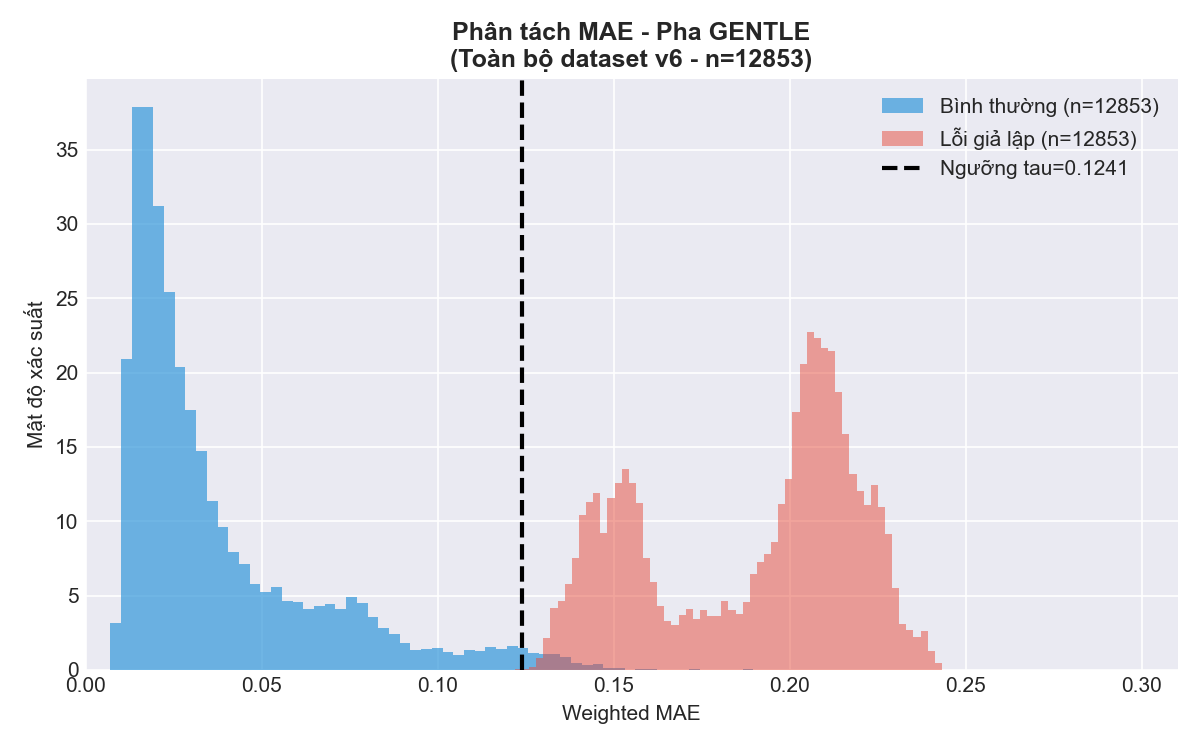
\includegraphics[width=\linewidth]{chap4/image/mae_sep_v11_GENTLE.png}
        \caption{Pha GENTLE ($n=12.853$)}
        \label{fig:mae_gentle}
    \end{subfigure}
    \hfill
    \begin{subfigure}[b]{0.32\textwidth}
        \centering
        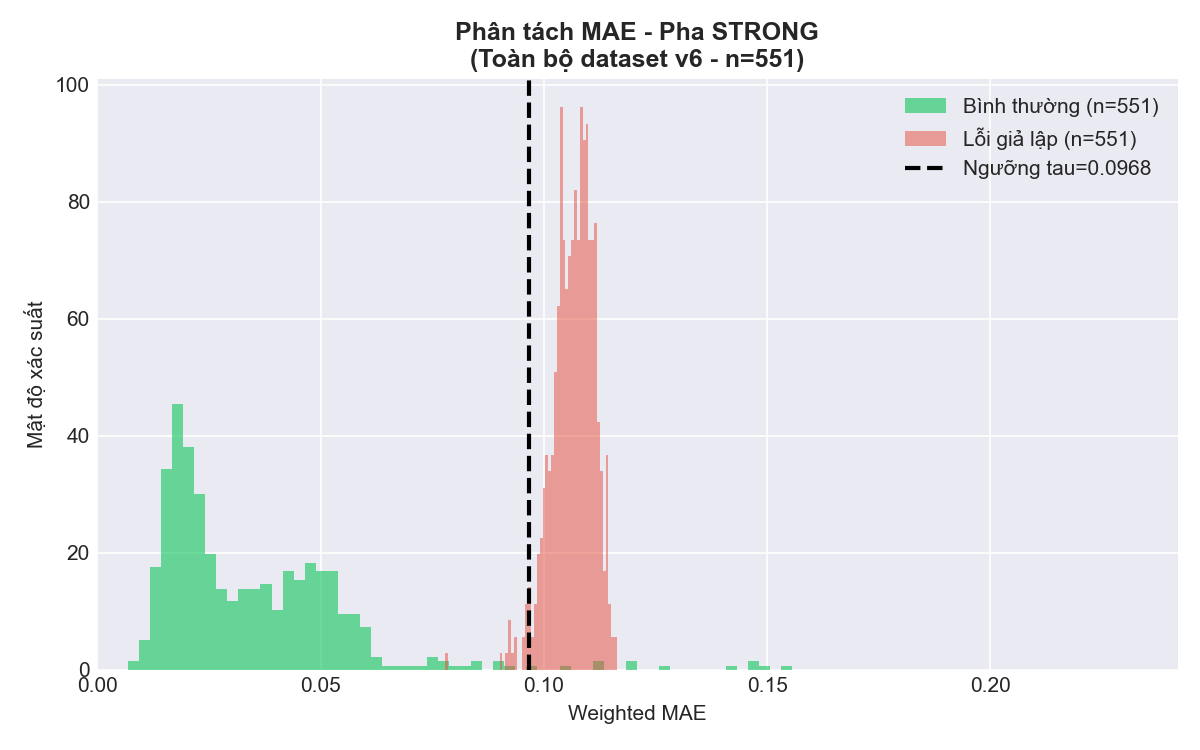
\includegraphics[width=\linewidth]{chap4/image/mae_sep_v11_STRONG.png}
        \caption{Pha STRONG ($n=551$)}
        \label{fig:mae_strong}
    \end{subfigure}
    \hfill
    \begin{subfigure}[b]{0.32\textwidth}
        \centering
        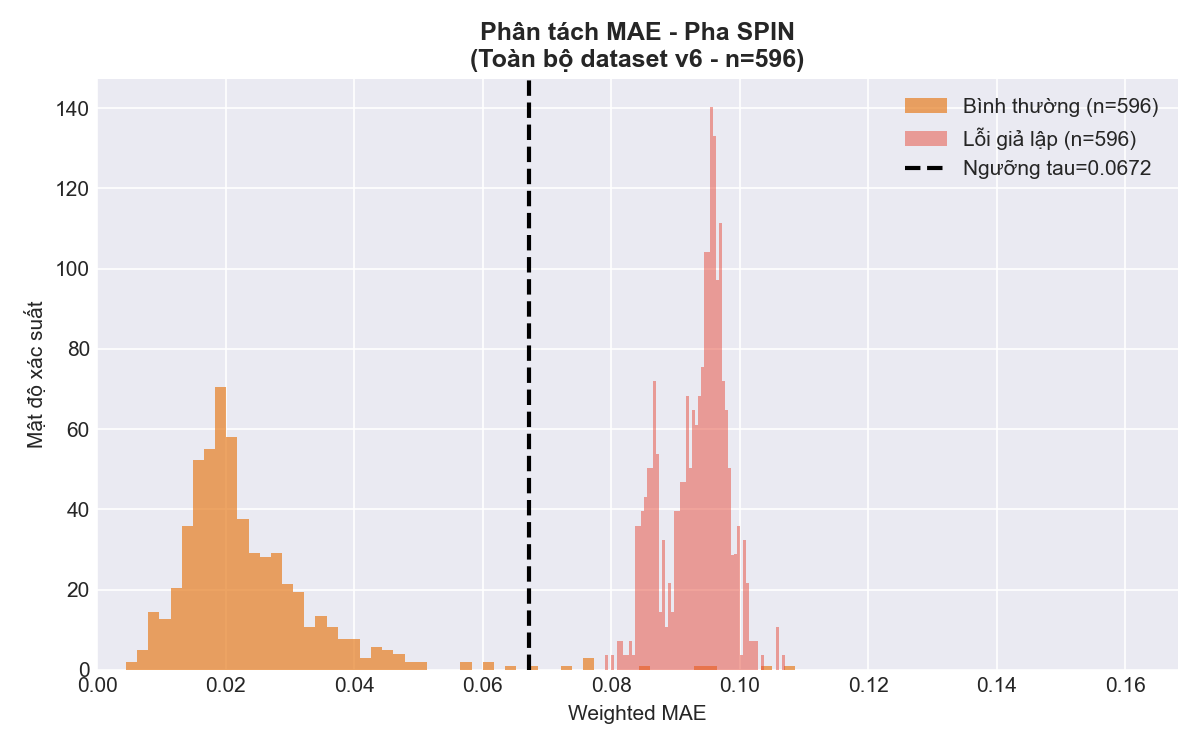
\includegraphics[width=\linewidth]{chap4/image/mae_sep_v11_SPIN.png}
        \caption{Pha SPIN ($n=596$)}
        \label{fig:mae_spin}
    \end{subfigure}
    \caption[Biểu đồ phân tách sai số MAE]{Biểu đồ phân tách sai số tái tạo MAE thực nghiệm trên mô hình v11. Mỗi pha vận hành được kiểm thử với tập dữ liệu tương ứng và tập lỗi giả lập ($n_{anomaly} \approx 500$ cho mỗi pha). Đường đứt nét biểu thị ngưỡng quyết định ($\tau$).}
    \label{fig:mae_sep_all}
\end{figure}

\subsection{Đánh giá độ nhạy và hiệu quả qua các chỉ số học máy}

Hiệu năng được đo lường qua chỉ số diện tích dưới đường cong ROC (AUC), F1-Score, Precision và Recall. Kết quả ghi nhận tại Bảng~\ref{tab:machine_learning_metrics}:

\begin{table}[H]
    \centering
    \caption[Chỉ số hiệu năng mô hình Ba trạng thái]{Chỉ số hiệu năng của mô hình tự mã hóa Ba trạng thái trên tập kiểm thử}
    \label{tab:machine_learning_metrics}
    \begin{tabular}{|l|c|c|c|c|}
    \hline
    \rowcolor[HTML]{EFEFEF}
    \textbf{Trạng thái} & \textbf{AUC} & \textbf{F1-Score} & \textbf{Precision} & \textbf{Recall} \\ \hline
    GENTLE & $0{,}9989$ & $0{,}9898$ & $0{,}9837$ & $0{,}9960$ \\ \hline
    STRONG & $0{,}9837$ & $0{,}9892$ & $0{,}9804$ & $0{,}9982$ \\ \hline
    SPIN   & $0{,}9993$ & $0{,}9967$ & $0{,}9933$ & $1{,}0000$ \\ \hline
    \end{tabular}
\end{table}

\subsection{Cơ chế lọc trễ thời gian và sự ổn định dài hạn}

Trong môi trường thực tế, sai số tức thời có thể vượt ngưỡng do nhiễu ngẫu nhiên. Vì vậy, firmware sử dụng cơ chế biểu quyết bất đối xứng đã trình bày tại Hình~\ref{fig:debounce_logic}: kích hoạt ALARM khi có ít nhất $5/10$ mẫu vượt ngưỡng và chỉ phục hồi về OK khi số mẫu vượt ngưỡng giảm xuống không quá $1/10$. Sự kết hợp giữa mô hình học sâu và bộ lọc thời gian giúp hệ thống phản ứng chính xác với các xung nhiễu, đảm bảo chỉ phát cảnh báo khi sự cố thực sự xảy ra.

\section{Phân tích thực nghiệm các quyết định thiết kế mô hình}
\label{sec:thuc_nghiem_thiet_ke}

Để xác nhận tính tối ưu của kiến trúc mạng nơ-ron tự mã hóa Ba trạng thái, hệ thống thực hiện các thí nghiệm bổ sung nhằm làm rõ vai trò của từng thành phần kỹ thuật.

\subsection{Lựa chọn kiến trúc mạng qua các giai đoạn thử nghiệm}

Trước khi chốt kiến trúc cuối cùng, đồ án đã thử nghiệm ba cấu trúc mạng ở giai đoạn mô phỏng trên Kaggle: Vanilla AE làm mốc cơ sở, 1D-CNN AE cho dữ liệu chuỗi thời gian và LSTM AE cho phụ thuộc thời gian dài. Các mô hình được đánh giá trên cùng tập dữ liệu đã tiền xử lý, cùng quy trình huấn luyện và cùng các tiêu chí gồm sai số tái tạo, dung lượng mô hình sau khi nén INT8 trên Kaggle, độ trễ suy luận mô phỏng trên Kaggle và độ bất ổn khi thêm nhiễu. Kết quả ban đầu cho thấy thứ tự hiệu quả là 1D-CNN AE, Vanilla AE và LSTM AE.

\begin{table}[H]
\centering
\caption[So sánh ba kiến trúc mạng sau nén INT8 trên Kaggle]{So sánh ba kiến trúc mạng ở giai đoạn mô phỏng sau khi nén INT8 trên Kaggle. Các giá trị trong bảng là số liệu mô phỏng, chưa phải kết quả đo trực tiếp trên phần cứng thực tế.}
\label{tab:network_architecture_comparison}
\renewcommand{\arraystretch}{1.15}
\begin{tabular}{lccc}
\toprule
\textbf{Chỉ số} & \textbf{Vanilla AE} & \textbf{1D-CNN AE} & \textbf{LSTM AE} \\
\midrule
RAE Loss (MSE) & $0{,}004947$ & \textbf{$0{,}003698$} & $0{,}004198$ \\
Dung lượng INT8 (KB) & $375{,}01$ KB & $30{,}52$ KB & $368{,}66$ KB \\
Độ trễ mô phỏng (ms/Kaggle) & $76{,}56$ ms & $79{,}73$ ms & $129{,}50$ ms \\
Bất ổn với nhiễu (\%) & $793{,}63\%$ & \textbf{$706{,}43\%$} & $722{,}42\%$ \\
\bottomrule
\end{tabular}
\end{table}

Từ Bảng~\ref{tab:network_architecture_comparison}, 1D-CNN AE là ứng viên tốt nhất ở giai đoạn mô phỏng vì đạt sai số tái tạo thấp nhất, dung lượng sau nén INT8 nhỏ nhất và độ bất ổn với nhiễu thấp nhất trong ba mô hình. Vanilla AE có độ trễ mô phỏng thấp hơn 1D-CNN AE một chút nhưng lại có sai số tái tạo, dung lượng INT8 và độ bất ổn với nhiễu cao hơn đáng kể. LSTM AE không phù hợp với yêu cầu nhúng do độ trễ mô phỏng cao nhất và dung lượng sau nén vẫn lớn.

Mặc dù 1D-CNN AE đứng đầu ở giai đoạn mô phỏng, quá trình triển khai thực tế trên TensorFlow Lite Micro cho thấy kiến trúc này không ổn định khi đưa xuống phần cứng. Nguyên nhân chính gồm sai lệch kết quả giữa triển khai Conv1D trên Python và C++, yêu cầu đầu vào dạng chuỗi làm tăng chi phí quản lý bộ đệm, và rủi ro mất ổn định khi chuyển toàn bộ mô hình sang INT8. Vì vậy, đồ án chuyển hướng sang Symmetric Dense AE kết hợp khối trích xuất đặc trưng DSP 19 chiều. Phương án này không phải là mô hình đứng đầu trong vòng so sánh mô phỏng ban đầu, mà là quyết định thiết kế sau khi cân nhắc đầy đủ tính khả thi triển khai trên vi điều khiển Seeed Studio XIAO ESP32-S3.

Sau khi tối ưu, kiến trúc Symmetric Dense AE sử dụng cấu trúc đối xứng $19 \rightarrow 128 \rightarrow 64 \rightarrow 32 \rightarrow 64 \rightarrow 128 \rightarrow 19$ với lớp thắt cổ chai Sigmoid, tương thích tốt với lượng tử hóa INT8. Tổng dung lượng ba mô hình cho ba pha vận hành là $95{,}3$ KB, độ trễ suy luận trung bình đo thực tế đạt $6{,}4$ ms, đáp ứng yêu cầu triển khai nhúng và được chọn cho hệ thống cuối cùng.

\subsection{Nghiên cứu thành phần các biến thể mô hình}
So sánh giữa mô hình ba trạng thái đề xuất với các biến thể cấu hình khác nhau giúp xác định hiệu quả của từng thành phần. Kết quả được tổng hợp trong Bảng~\ref{tab:ablation_study}.

\begin{table}[H]
\centering
\caption[So sánh hiệu năng các biến thể mô hình]{So sánh hiệu năng giữa các biến thể mô hình trong nghiên cứu thành phần. (*) Trễ trung bình đo thực tế trên vi điều khiển Seeed Studio XIAO ESP32-S3 với N=1\,000 lần.}
\label{tab:ablation_study}
\begin{adjustbox}{max width=\textwidth}
\begin{tabular}{|l|c|c|c|c|}
\hline
\textbf{Biến thể} & \textbf{MAE (SPIN)} & \textbf{F1-Score} & \textbf{Trễ ($ms$)} & \textbf{Model Flash (KB)} \\ \hline
Mô hình đơn AE (Chung 3 pha) & 0,0421 & 0,845 & 6,5 & 31,7 \\ \hline
Ba trạng thái AE (Không dùng MAE có trọng số) & 0,0291 & 0,912 & 6,4* & 95,3 \\ \hline
\textbf{Ba trạng thái AE đề xuất} & \textbf{0,0242} & \textbf{0,9967} & \textbf{6,4*} & \textbf{95,3} \\ \hline
\end{tabular}
\end{adjustbox}
\end{table}

Kiến trúc Ba trạng thái đem lại bước nhảy lớn nhất về hiệu năng. Biến thể mô hình đơn sử dụng chung một mô hình cho cả 3 pha chỉ đạt F1-Score 0,845, thấp hơn đáng kể so với Ba trạng thái, cho thấy mỗi pha có đặc tính thống kê riêng biệt. Bên cạnh đó, hàm mất mát MAE có trọng số (trọng số rung động gấp 5 lần âm thanh) nâng F1 từ 0,912 lên 0,9967 ở pha SPIN, khẳng định tầm quan trọng của việc ưu tiên kênh cảm biến mang tính vật lý cao hơn.

Kích thước lớp thắt cổ chai ảnh hưởng trực tiếp đến khả năng nén đặc trưng và tài nguyên tính toán. Khảo sát các kích thước tiềm năng tìm ra kích thước tối ưu (Bảng~\ref{tab:bottleneck_sweep}).

\begin{table}[H]
\centering
\caption[Kết quả khảo sát lớp thắt cổ chai]{Kết quả khảo sát kích thước lớp thắt cổ chai. \textit{Lưu ý: Các giá trị độ trễ (ms) trong bảng là ước tính tương đối dùng để so sánh tỷ lệ tài nguyên.}}
\label{tab:bottleneck_sweep}
\begin{tabular}{|c|c|c|c|c|}
\hline
\textbf{Số chiều} & \textbf{MAE (TB)} & \textbf{Tham số} & \textbf{Trễ ($ms$)} & \textbf{Đánh giá} \\ \hline
8 & 0,0321 & 19.347 & 5,8 & Underfitting \\ \hline
16 & 0,0265 & 22.563 & 6,1 & Đạt yêu cầu \\ \hline
\textbf{32} & \textbf{0,0242} & \textbf{25.779} & \textbf{6,4} & \textbf{Điểm tối ưu} \\ \hline
64 & 0,0241 & 32.211 & 7,4 & Bão hòa \\ \hline
\end{tabular}
\end{table}

Tại 32 chiều, mô hình đạt hiệu năng tối ưu. Tăng lên 64 chiều chỉ giảm sai số MAE không đáng kể nhưng tăng 15\% độ trễ suy luận và dung lượng bộ nhớ. 32 chiều là lựa chọn tối ưu cho vi điều khiển Seeed Studio XIAO ESP32-S3.

\subsection{Phân tích ngưỡng $\tau$ bằng đường cong ROC và chỉ số Youden's J}
Phân tích đường cong ROC tối ưu hóa khả năng phân tách giữa dữ liệu bình thường và bất thường (Hình~\ref{fig:roc_all_states}).

\begin{figure}[H]
    \centering
    \begin{subfigure}{0.32\textwidth}
        \centering
        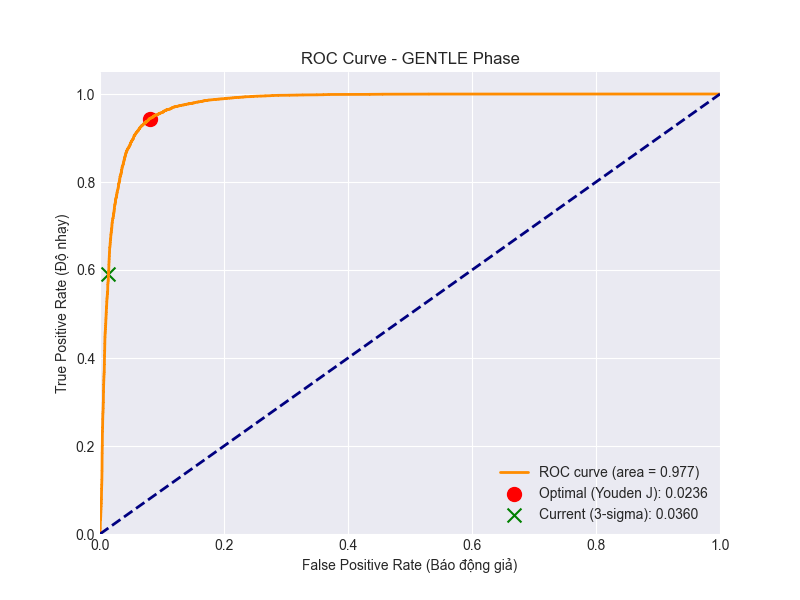
\includegraphics[width=\linewidth]{chap4/image/roc_gentle.png}
        \caption{GENTLE}
    \end{subfigure}
    \hfill
    \begin{subfigure}{0.32\textwidth}
        \centering
        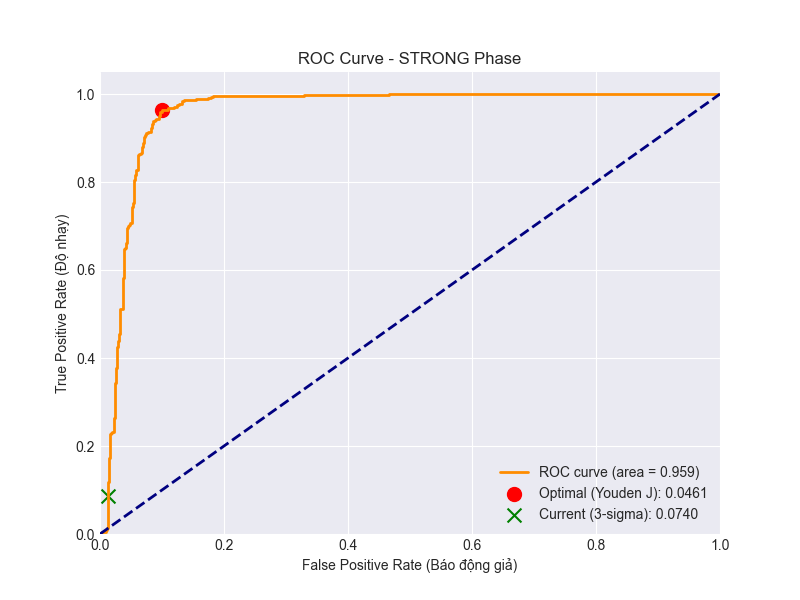
\includegraphics[width=\linewidth]{chap4/image/roc_strong.png}
        \caption{STRONG}
    \end{subfigure}
    \hfill
    \begin{subfigure}{0.32\textwidth}
        \centering
        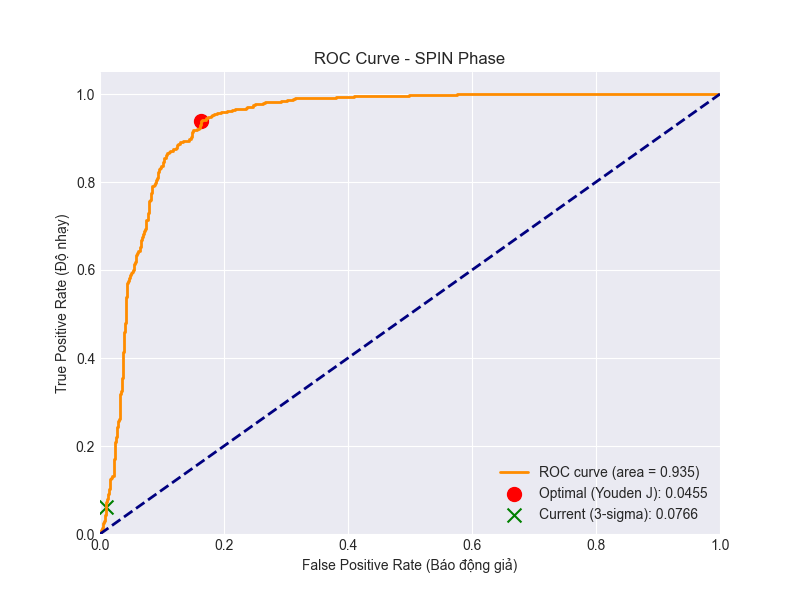
\includegraphics[width=\linewidth]{chap4/image/roc_spin.png}
        \caption{SPIN}
    \end{subfigure}
    \caption[Đường cong ROC ba pha vận hành]{Đường cong ROC và điểm Youden's J Index tối ưu cho ba pha vận hành GENTLE, STRONG và SPIN.}
    \label{fig:roc_all_states}
\end{figure}

Diện tích dưới đường cong (AUC) đạt: GENTLE (0,9989), STRONG (0,9837), SPIN (0,9993). Thông qua chỉ số Youden's J ($J = Sensitivity + Specificity - 1$), chúng tôi xác định ngưỡng $\tau_{optimal}$. Tuy nhiên, trong thiết kế thực tế, hệ thống ưu tiên ngưỡng thống kê $3\sigma$ (nghiêm ngặt hơn Youden) để giảm cảnh báo giả và tránh ảnh hưởng tiêu cực đến người dùng trong môi trường dân dụng.

Tại ngưỡng $3\sigma$, độ chính xác (Precision) đạt 0,99 ở cả 3 pha, nhưng chỉ số Recall ở pha GENTLE giảm xuống 0,78 so với 0,91 tại điểm Youden. Đây là sự đánh đổi kỹ thuật nhằm đảm bảo độ ổn định của hệ thống cảnh báo trước các nhiễu môi trường.

\subsection{Phân tích sâu nguyên nhân sai số pha GENTLE}
Pha STRONG có AUC thấp nhất (0,9837), trong khi pha GENTLE vẫn là chế độ dễ phát sinh nhiễu nền do cường độ vận hành thấp. Phân tích các mẫu bị nhận diện sai cho thấy hai vấn đề chính:

\begin{itemize}
    \item \textbf{False Negatives:} Xảy ra khi biến động gia tốc trục Z cực nhỏ (MAE xấp xỉ ngưỡng bình thường). Ở mức năng lượng này, đặc trưng rung động của lỗi bị lấn át bởi nhiễu nền của động cơ Inverter, khiến mạng nơ-ron tự mã hóa tái tạo lỗi như tín hiệu bình thường.
    \item \textbf{False Positives:} Chủ yếu do các nhiễu âm thanh đột biến từ môi trường bên ngoài (tiếng va chạm vật lý vào vỏ máy) không thuộc chu kỳ vận hành của máy giặt nhưng trùng vào dải tần số bộ lọc Mel mà mô hình giám sát.
\end{itemize}

\section{Triển khai ứng dụng di động giám sát và cảnh báo thời gian thực}
\label{sec:trien_khai_app}

Để hoàn thiện giải pháp AIoT từ biên đến đám mây, ứng dụng di động đa nền tảng được phát triển trên khung Flutter. Flutter là khung phát triển giao diện mã nguồn mở sử dụng mô hình giao diện khai báo, trong đó giao diện được xây dựng từ các thành phần tiện ích và tự cập nhật khi trạng thái dữ liệu thay đổi \citeweb{ref_flutter_docs}. Đặc điểm này phù hợp với bài toán giám sát thời gian thực, nơi trạng thái máy giặt, sai số tái tạo và cảnh báo có thể thay đổi liên tục theo luồng MQTT. Ứng dụng hoạt động như trạm giám sát trung tâm, cho phép người dùng theo dõi tình trạng máy giặt từ xa và nhận cảnh báo tức thời.

% ============================================================
\subsection{Kiến trúc phần mềm và kết nối đám mây}
% ============================================================

Ứng dụng sử dụng kiến trúc hướng sự kiện, duy trì kết nối với hai nền tảng đám mây, như minh họa tại Hình~\ref{fig:app_architecture}.

\begin{figure}[H]
    \centering
    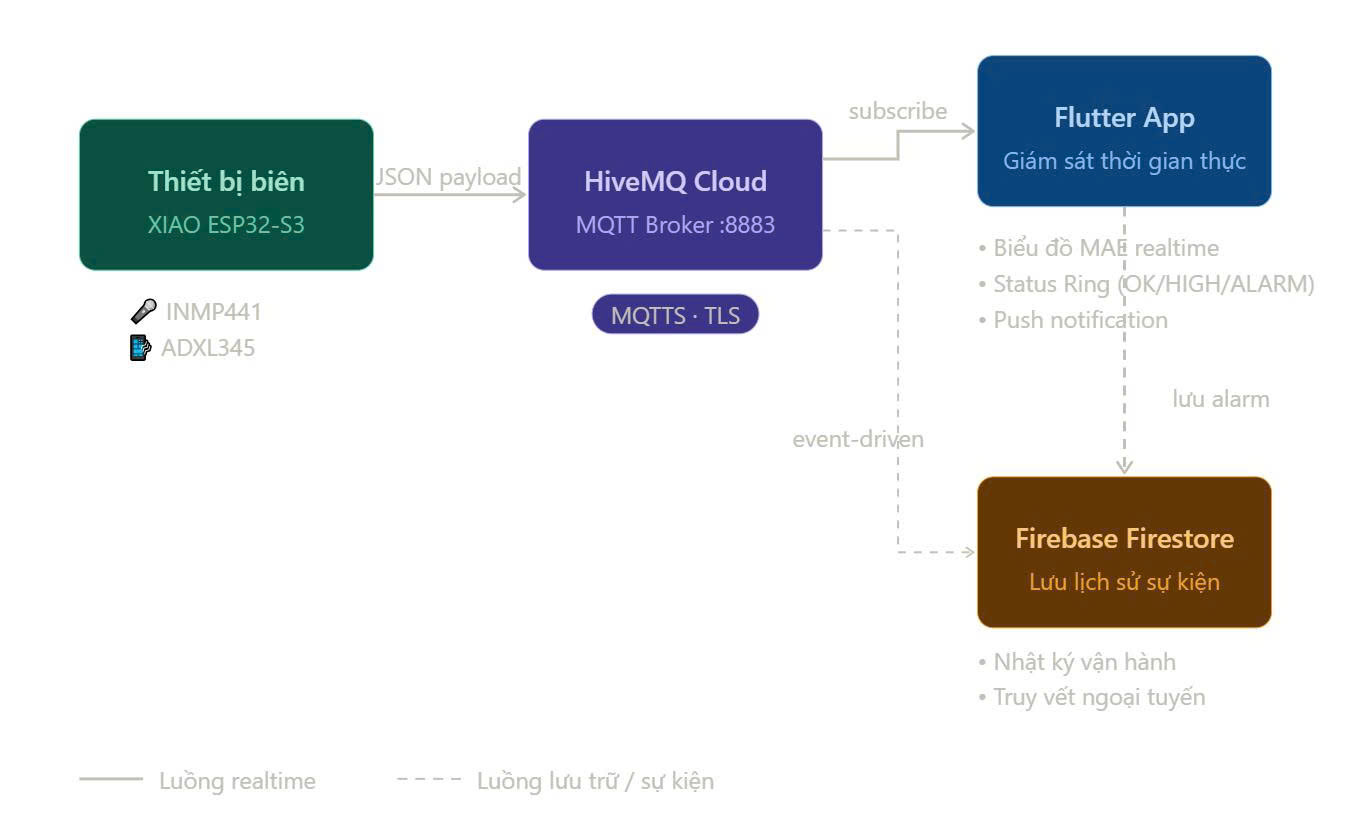
\includegraphics[width=0.85\textwidth]{chap4/image/app_architecture.png}
    \caption[Kiến trúc kết nối đám mây của ứng dụng di động]{Sơ đồ kiến trúc kết nối đám mây của ứng dụng di động. Dữ liệu từ thiết bị biên được phân phát theo hai nhánh độc lập: nhánh thời gian thực qua MQTT tới giao diện người dùng và nhánh lưu trữ lâu dài qua Firebase Firestore.}
    \label{fig:app_architecture}
\end{figure}

\textbf{HiveMQ Cloud} tiếp nhận luồng dữ liệu thời gian thực từ thiết bị biên với vai trò máy chủ trung gian MQTT. Dữ liệu được đóng gói theo định dạng JSON và truyền qua cổng 8883 (MQTTS), đảm bảo bảo mật và giữ độ trễ thấp.

\textbf{Firebase Firestore} lưu trữ lịch sử các sự kiện bất thường. Firestore là cơ sở dữ liệu NoSQL tổ chức dữ liệu theo các bộ sưu tập và tài liệu, phù hợp với dữ liệu vận hành có cấu trúc linh hoạt như thời điểm cảnh báo, pha vận hành, giá trị MAE và trạng thái xử lý \citeweb{ref_firestore_docs}. Người dùng có thể tra cứu nhật ký vận hành và mốc thời gian lỗi ngay cả khi thiết bị biên ngoại tuyến; điều này hỗ trợ bảo trì theo lịch.

% ============================================================
\subsection{Logic xử lý dữ liệu và thông báo đẩy}
% ============================================================

Ứng dụng sử dụng bộ lắng nghe MQTT để xử lý dữ liệu. Mỗi khi nhận gói tin từ chủ đề \texttt{tinyml/quang\_wm\_2026/status}, ứng dụng thực hiện ba bước: giải mã tải tin JSON để trích xuất các trường \texttt{is\_alarm}, \texttt{mae} và \texttt{mode}; kích hoạt thông báo đẩy ưu tiên cao nếu phát hiện cảnh báo, kèm đầy đủ giá trị MAE và pha vận hành; ghi nhận sự kiện vào Firestore. Song song đó, biểu đồ MAE trên giao diện được cập nhật liên tục.

Thông báo được tạo thông qua thư viện \texttt{flutter\_local\_notifications} với mức ưu tiên cao, bao gồm giá trị MAE và pha vận hành tại thời điểm xảy ra lỗi. Đo đạc độ trễ từ đầu đến cuối — từ khi vi điều khiển phát hiện bất thường đến khi thông báo xuất hiện — ghi nhận mức xấp xỉ \textbf{2,0 giây}. Thời gian này bao gồm độ trễ MQTT qua máy chủ trung gian và phản hồi của hệ điều hành, đáp ứng yêu cầu giám sát thời gian thực cho thiết bị gia dụng. Hình~\ref{fig:notification} minh họa thông báo đẩy trên Android.

\begin{figure}[H]
    \centering
    \begin{subfigure}[b]{0.42\textwidth}
        \centering
        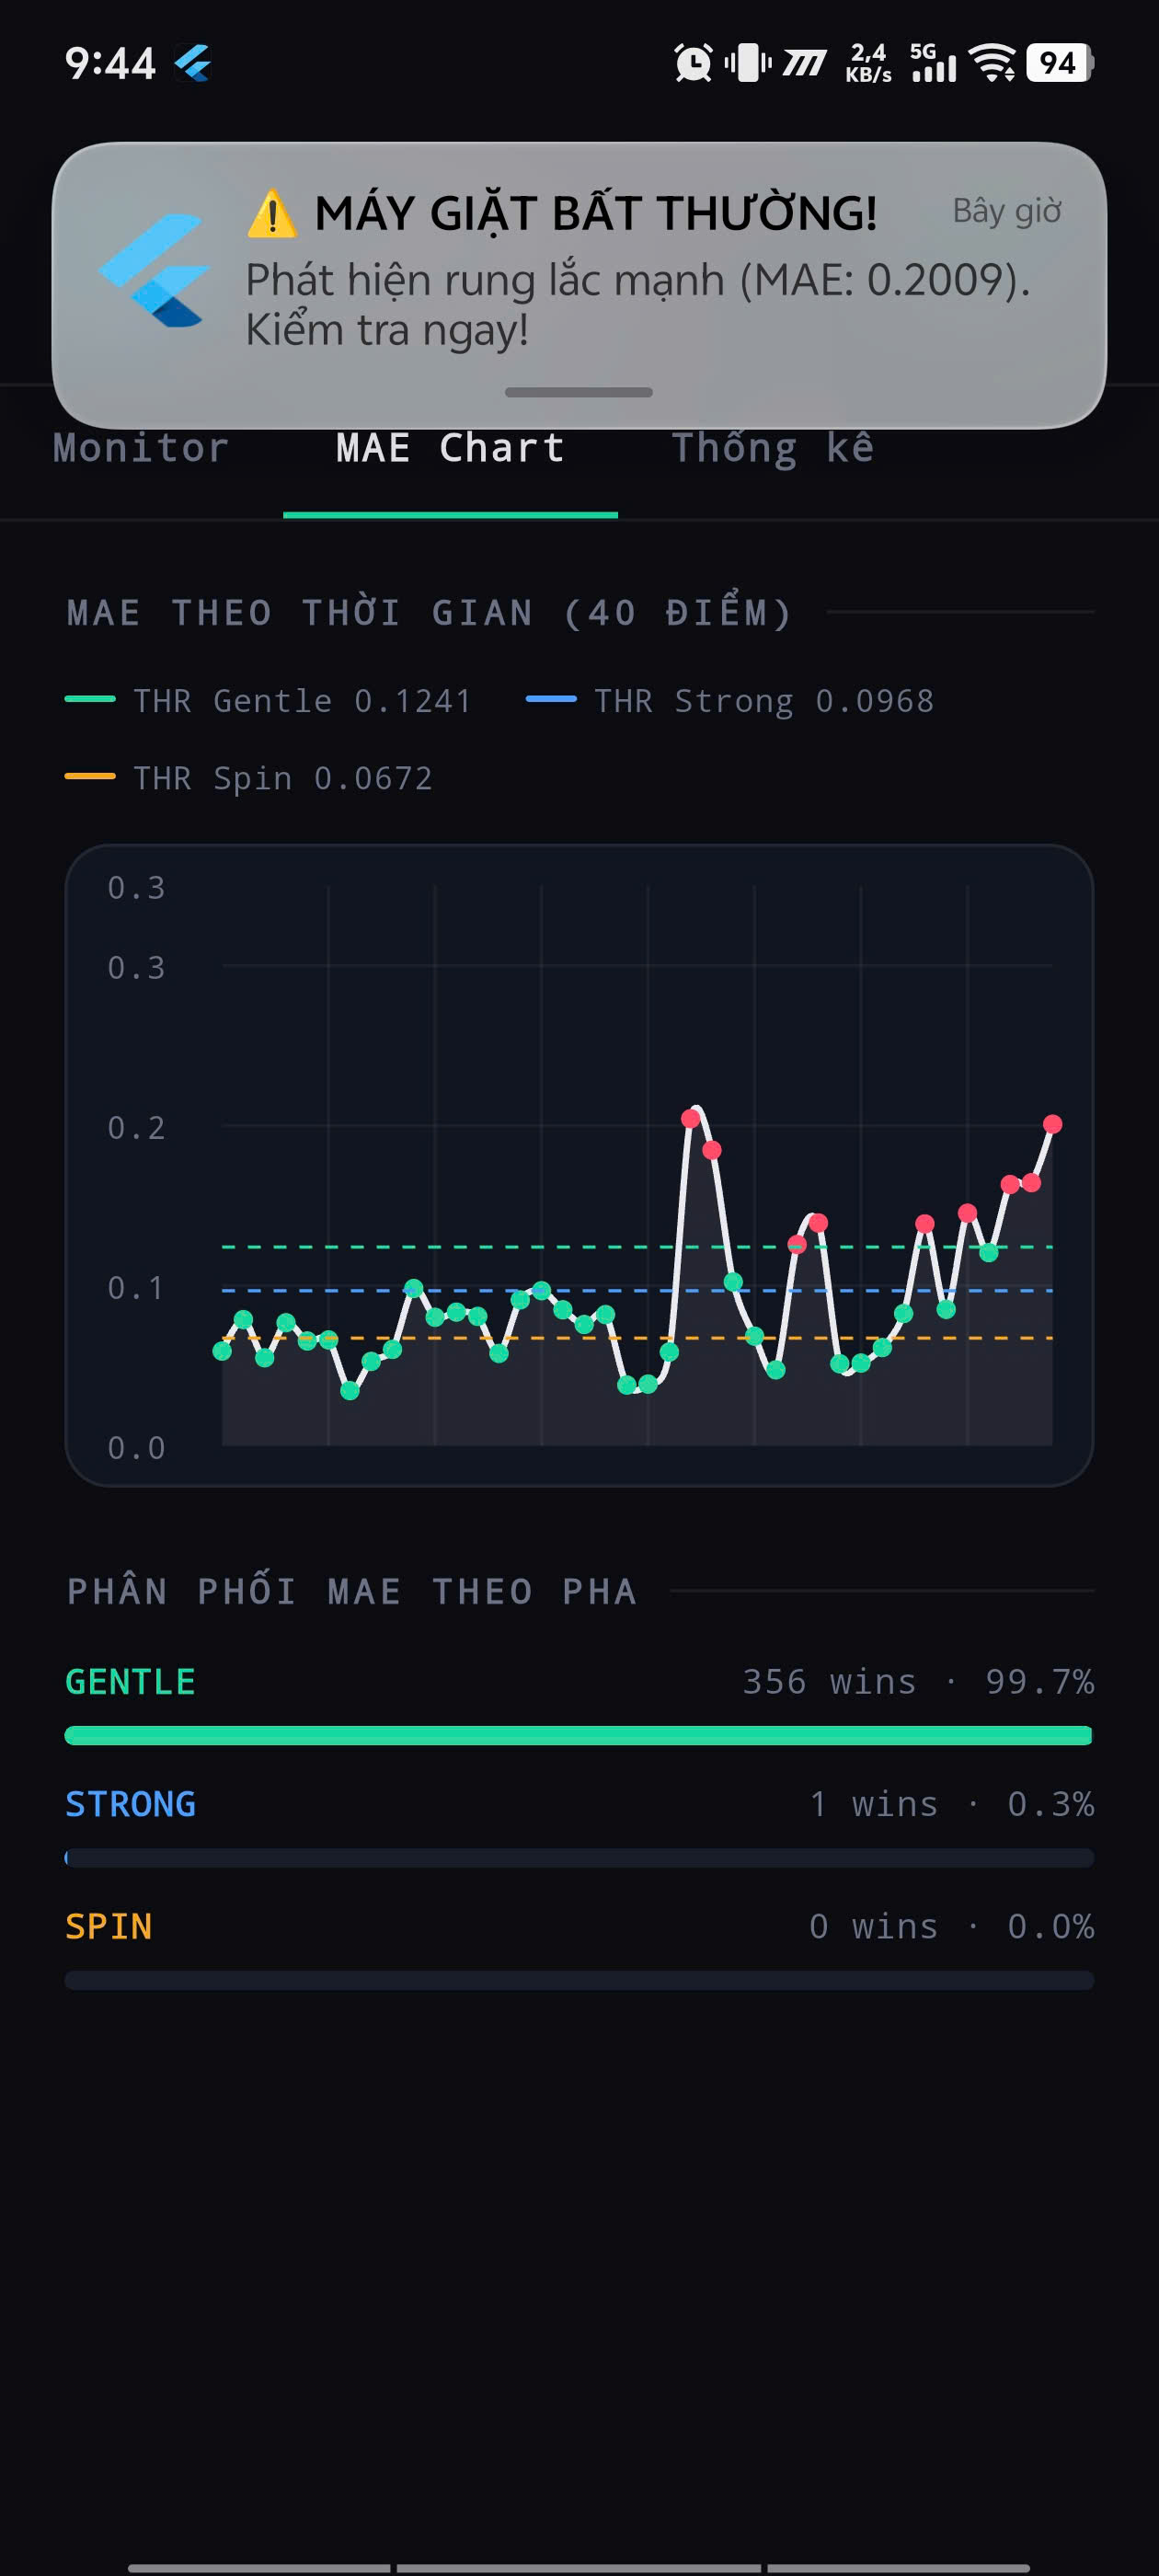
\includegraphics[width=\linewidth]{chap4/image/notification_banner.png}
        \caption{Thông báo dạng banner xuất hiện phía trên màn hình khi ứng dụng đang mở.}
        \label{fig:notif_banner}
    \end{subfigure}
    \hfill
    \begin{subfigure}[b]{0.42\textwidth}
        \centering
        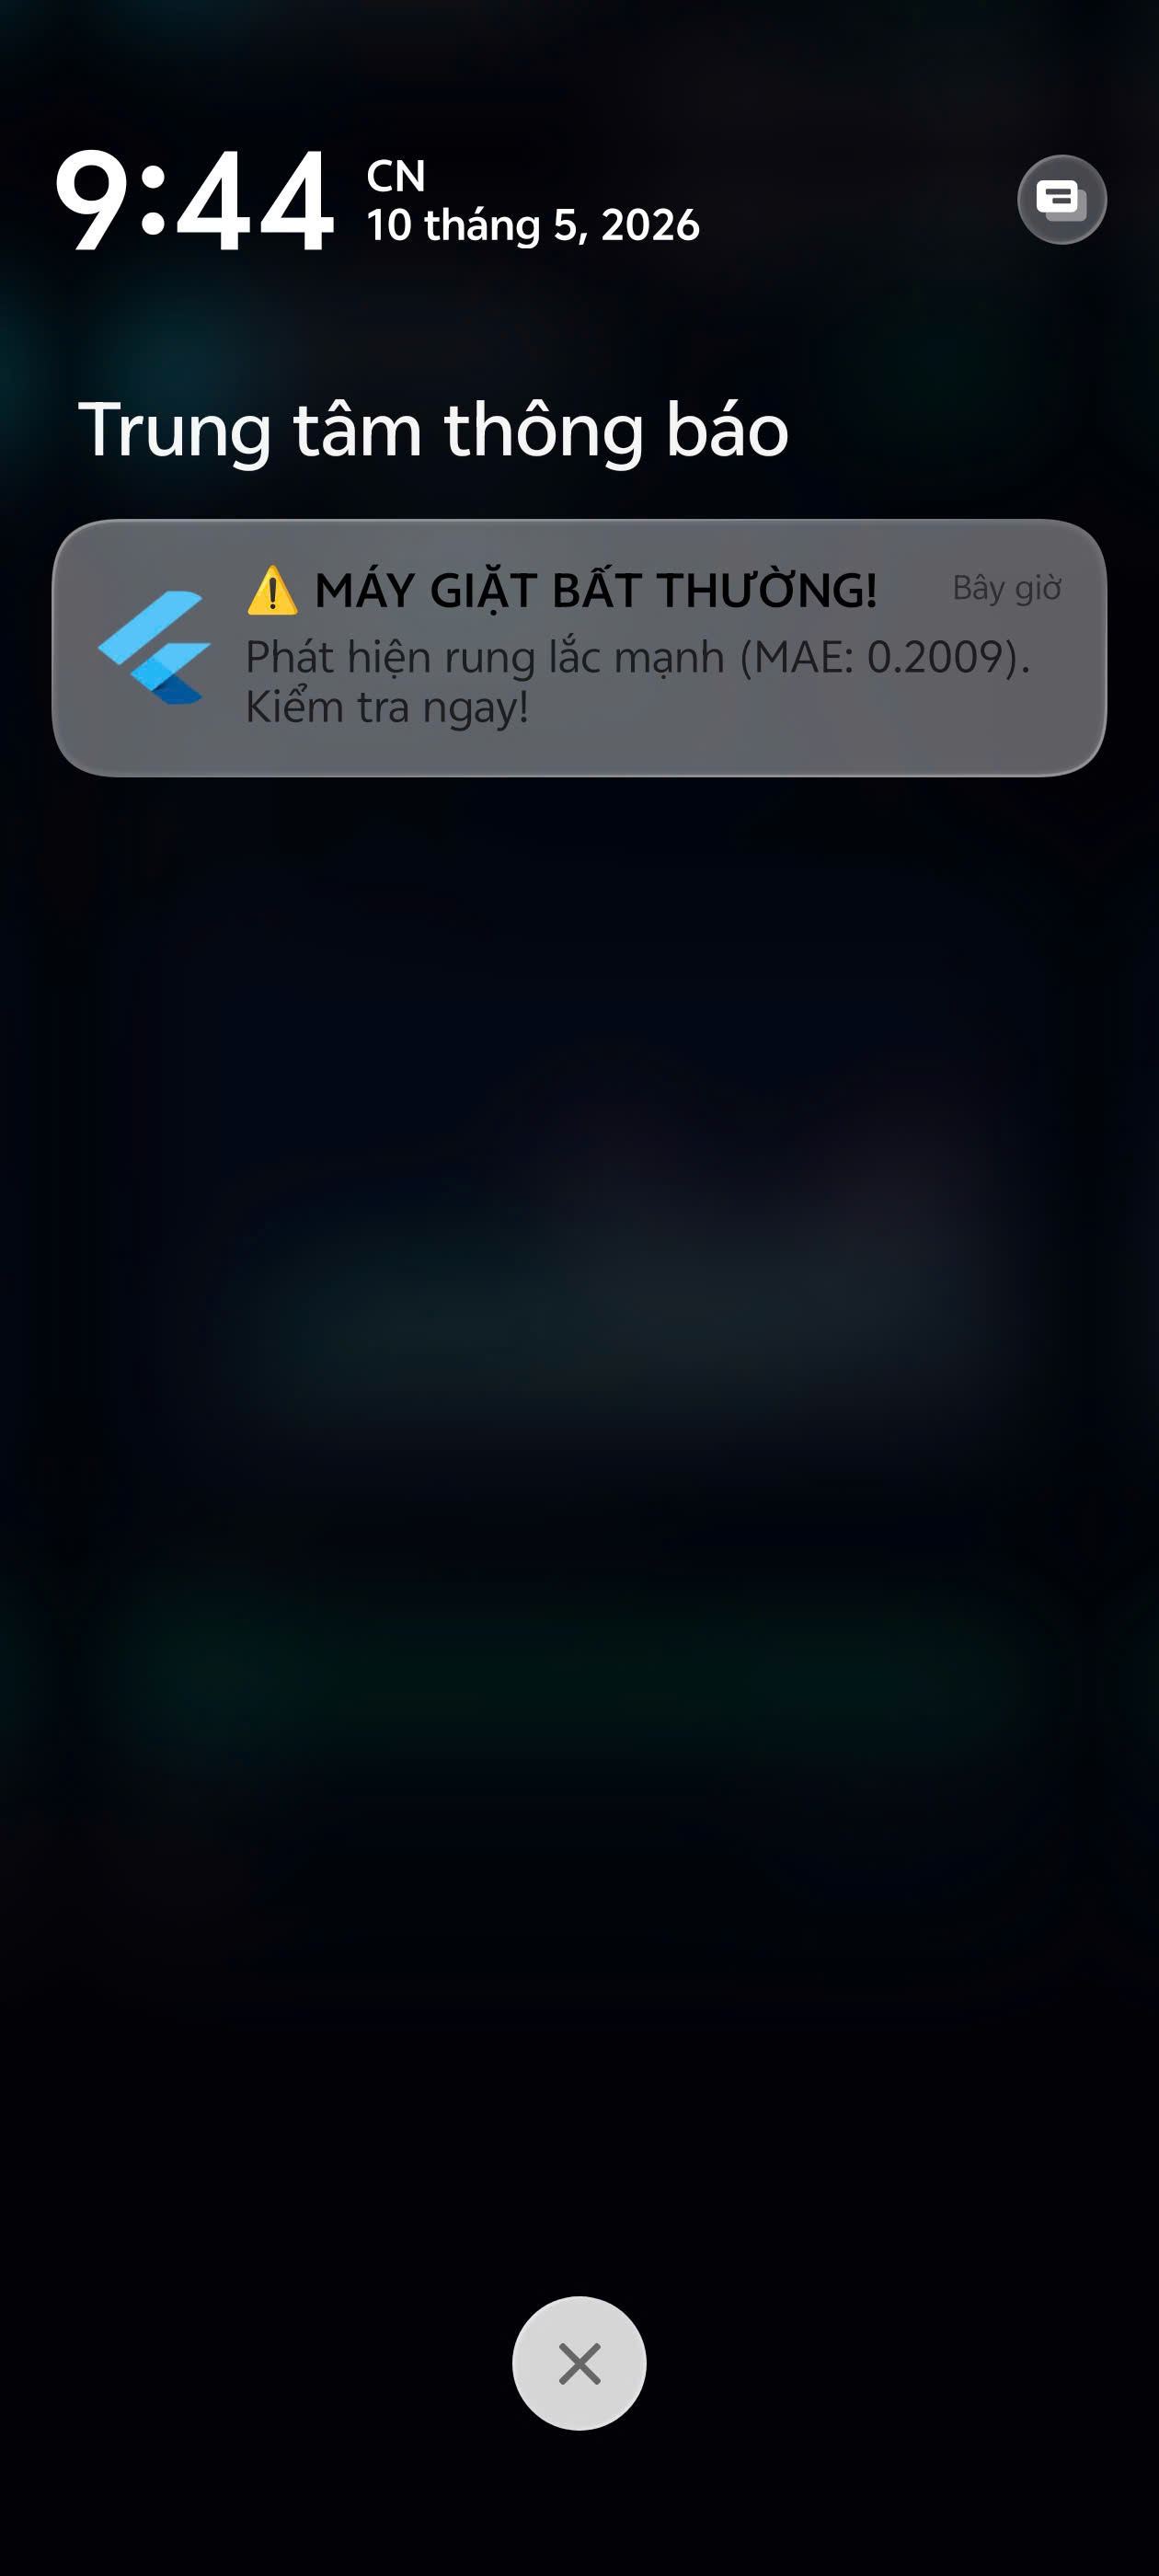
\includegraphics[width=\linewidth]{chap4/image/notification_lockscreen.png}
        \caption{Thông báo hiển thị tại Trung tâm thông báo khi thiết bị đang khóa màn hình.}
        \label{fig:notif_lockscreen}
    \end{subfigure}
    \caption[Minh họa thông báo đẩy trên Android]{Thông báo đẩy thực tế trên Android khi hệ thống kích hoạt ALARM --- "Phát hiện rung lắc mạnh (MAE: 0.2009). Kiểm tra ngay!". Thông báo được gửi trong vòng \textbf{2,0 giây} kể từ khi vi điều khiển phát hiện bất thường.}
    \label{fig:notification}
\end{figure}

\subsection{Giao diện người dùng và trực quan hóa dữ liệu}
% ============================================================

Giao diện sử dụng chế độ tối hiện đại, tổ chức thành ba phần chức năng như tại Hình~\ref{fig:app_ui}.

\begin{figure}[H]
    \centering
    \begin{subfigure}[b]{0.32\textwidth}
        \centering
        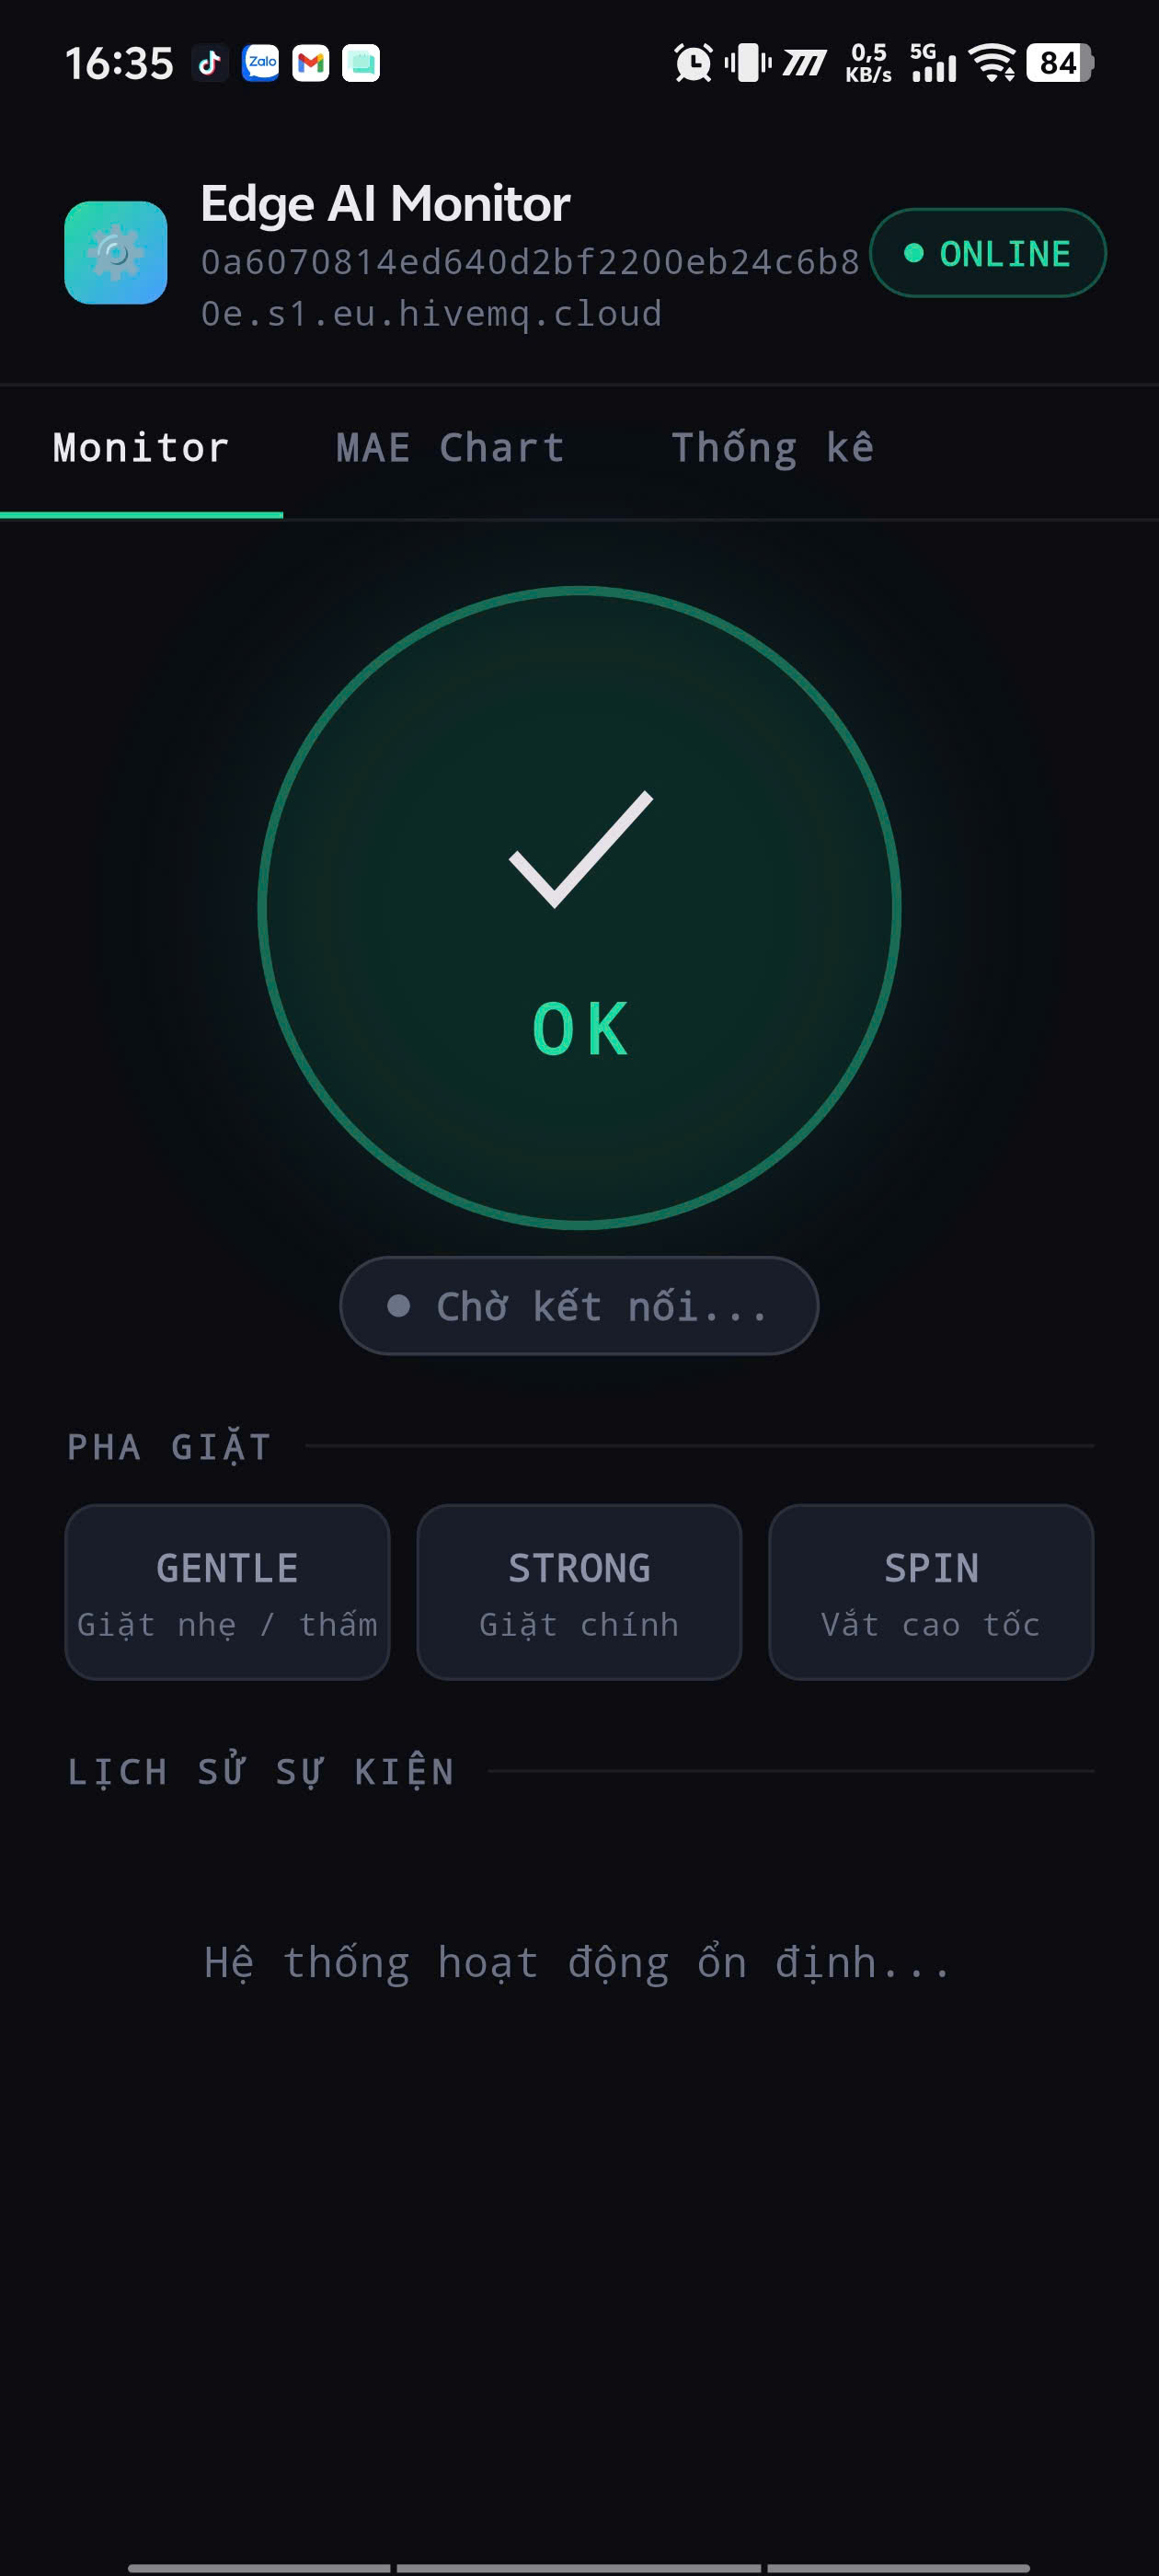
\includegraphics[width=\linewidth]{chap4/image/app_monitor.png}
        \caption{Màn hình Giám sát}
        \label{fig:ui_monitor}
    \end{subfigure}
    \hfill
    \begin{subfigure}[b]{0.32\textwidth}
        \centering
        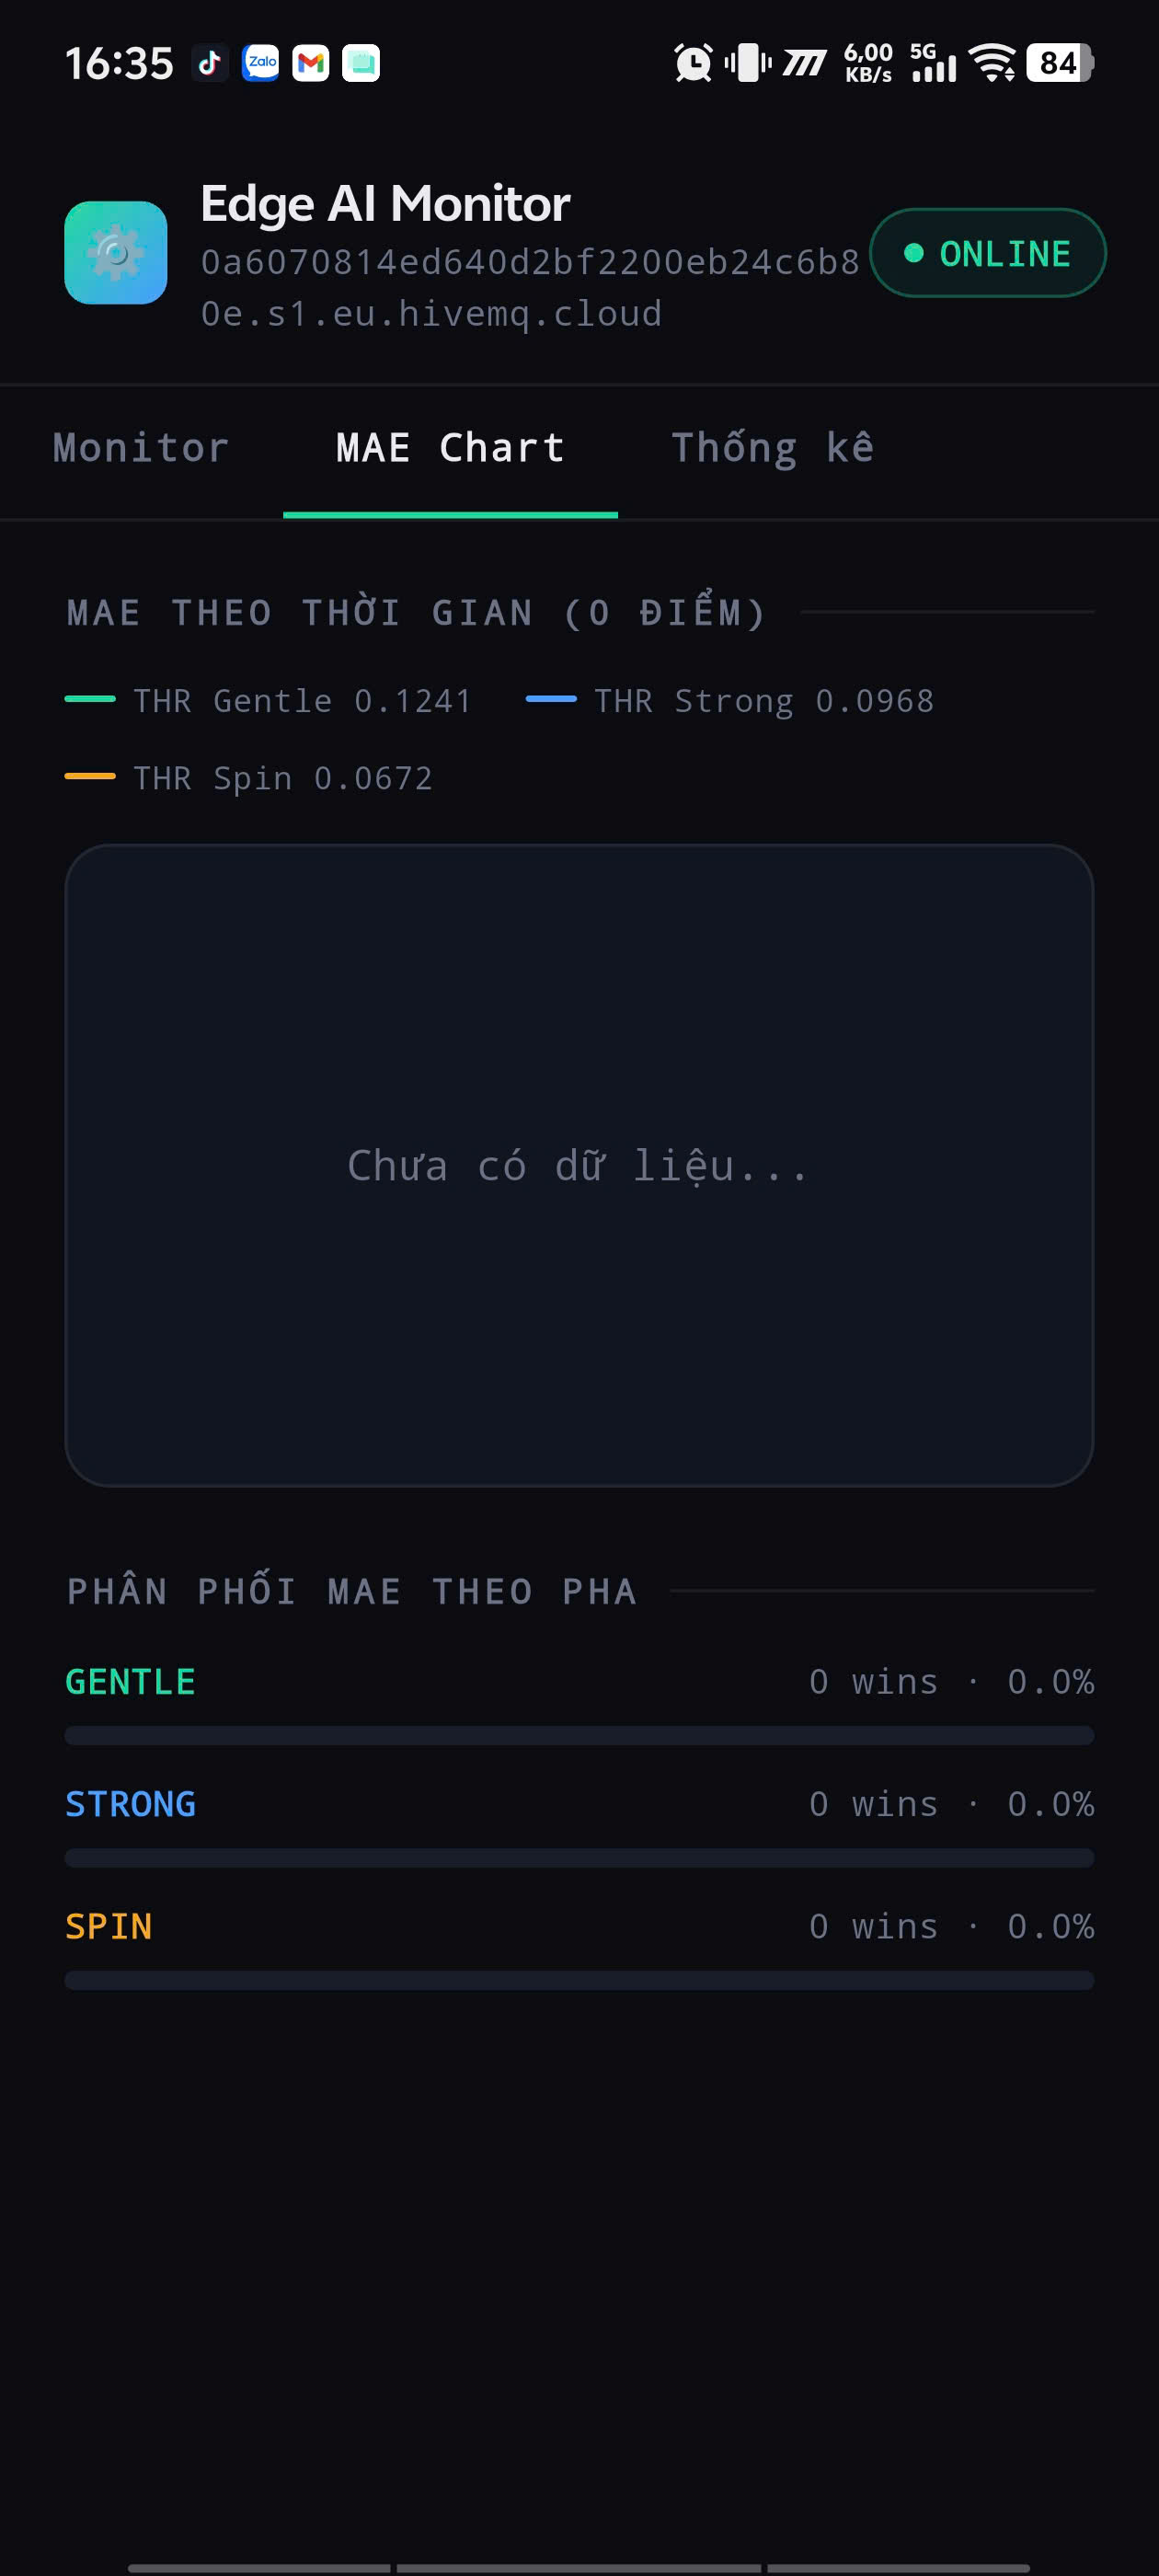
\includegraphics[width=\linewidth]{chap4/image/app_mae_chart.png}
        \caption{Biểu đồ MAE}
        \label{fig:ui_chart}
    \end{subfigure}
    \hfill
    \begin{subfigure}[b]{0.32\textwidth}
        \centering
        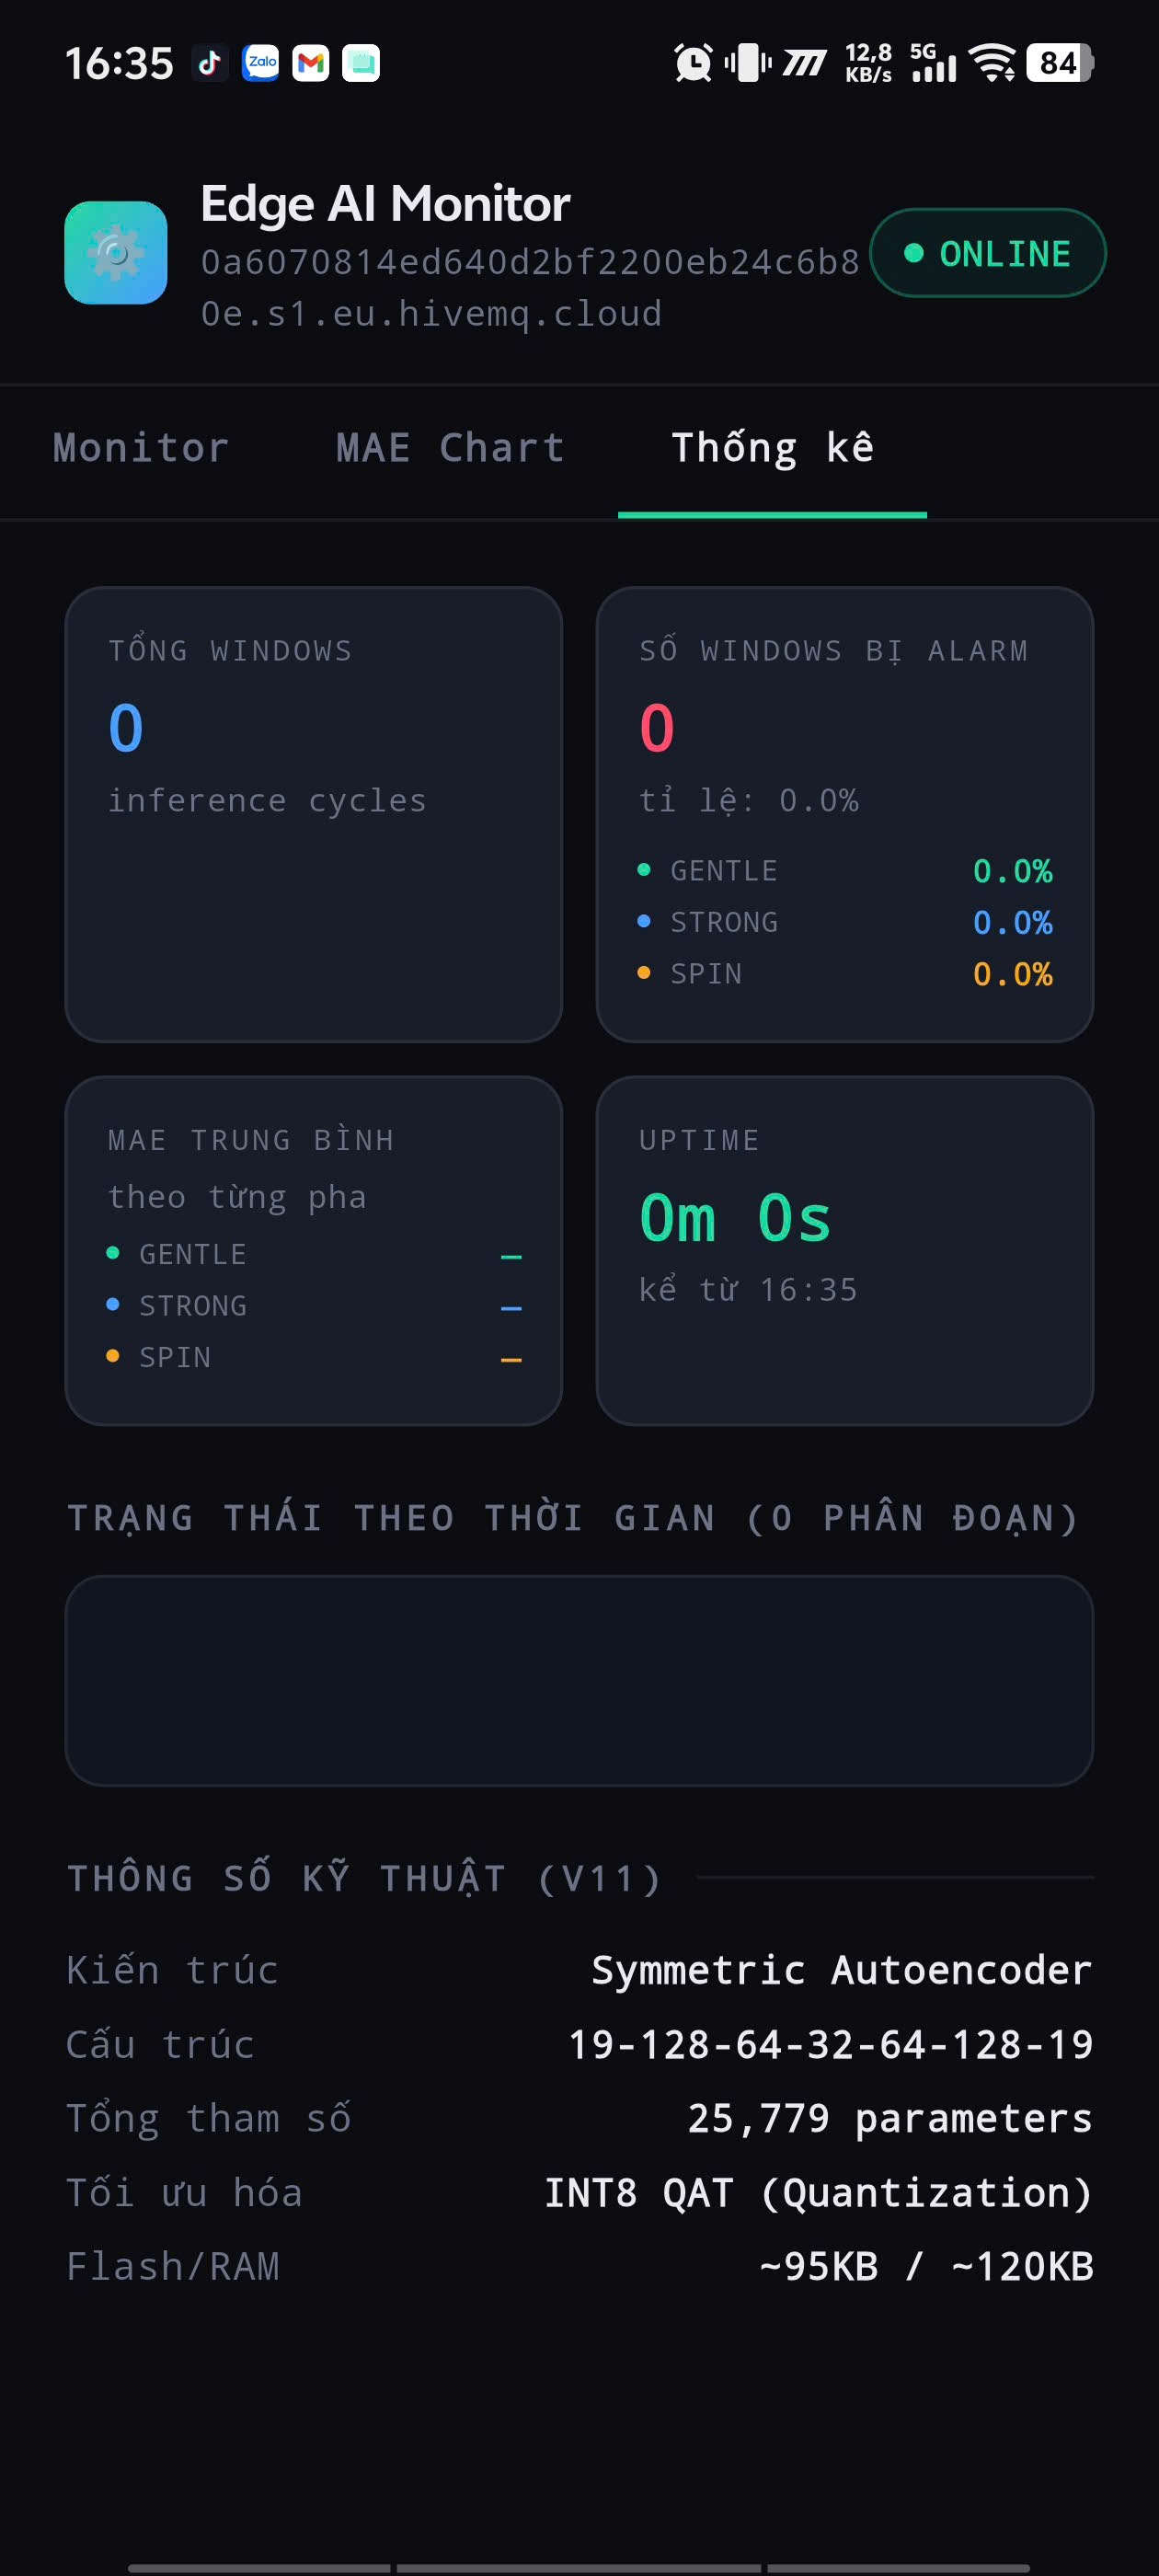
\includegraphics[width=\linewidth]{chap4/image/app_stats.png}
        \caption{Thống kê và Thông số}
        \label{fig:ui_stats}
    \end{subfigure}
    \caption[Giao diện ứng dụng di động Flutter]{Giao diện ứng dụng di động Flutter: (a) Vòng tròn trạng thái động; (b) Trực quan hóa sai số MAE cùng các đường ngưỡng $\tau$ tương ứng; (c) Bảng thống kê nhật ký vận hành và thông số mô hình thực tế.}
    \label{fig:app_ui}
\end{figure}

\textbf{Màn hình Giám sát (Monitor)} hiển thị vòng tròn trạng thái động thay đổi màu sắc: xanh lá ứng với trạng thái bình thường (OK), vàng khi sai số tiệm cận ngưỡng (HIGH), đỏ khi kích hoạt cảnh báo (ALARM). Cơ chế này giúp người dùng nhận biết tình trạng máy trong một cái nhìn mà không cần đọc số liệu kỹ thuật.

\textbf{Biểu đồ MAE thời gian thực} được dựng bằng thư viện \texttt{fl\_chart}, thể hiện sai số tái tạo theo thời gian. Đường ngưỡng $\tau$ tương ứng với pha vận hành hiện tại được vẽ chồng lên dạng đường đứt nét làm tham chiếu. Quan sát xu hướng MAE trước khi chạm ngưỡng có giá trị thực tiễn: người dùng có thể nhận diện sớm dấu hiệu bất thường đang tích lũy và kiểm tra thiết bị trước khi lỗi trở nên nghiêm trọng.

\textbf{Màn hình Thống kê và Nhật ký} tổng hợp số lượng cảnh báo theo từng pha vận hành (GENTLE, STRONG, SPIN), hỗ trợ người dùng đánh giá xu hướng hao mòn của thiết bị theo các chế độ giặt khác nhau trong dài hạn.

Lớp ứng dụng di động này hoàn thiện vòng phản hồi của hệ thống AIoT và kết nối các thuật toán TinyML phức tạp với người dùng cuối, giúp các chỉ số kỹ thuật trở thành thông tin cảnh báo có ý nghĩa thực tiễn và dễ tiếp cận.

\section{So sánh với các nghiên cứu liên quan}
\label{sec:so_sanh_baseline}

\subsection{Giới thiệu hệ thống mốc đối sánh của Mansoureh Lord}

Nghiên cứu của Mansoureh Lord (2021) \cite{ref_1_lord} là luận văn thạc sĩ tiêu biểu tại Sabancı University, tập trung phát hiện lỗi mất cân bằng lồng giặt trên máy giặt cửa trên sử dụng cảm biến gia tốc ADXL345 và mô hình tự mã hóa đơn giản một lớp ẩn. Hệ thống đạt độ chính xác khoảng 94,3\% ở pha vắt nhưng chưa tích hợp kênh âm thanh và chưa triển khai cơ chế chuyển đổi trạng thái tự động. Trong phần này, công trình của Mansoureh Lord được sử dụng làm hệ thống mốc đối sánh trực tiếp.

Nghiên cứu này được lựa chọn làm mốc đối sánh vì:
\begin{itemize}
    \item Cùng bài toán phát hiện bất thường trên máy giặt
    \item Sử dụng phần cứng cảm biến tương tự (ADXL345)
    \item Áp dụng kiến trúc mạng tự mã hóa cho bài toán phát hiện bất thường
    \item Công bố kết quả định lượng rõ ràng
\end{itemize}

Để xác nhận giá trị đóng góp, hệ thống tự mã hóa ba trạng thái được so sánh với nghiên cứu của Mansoureh Lord (2021) \cite{ref_1_lord} — công trình tiêu biểu ứng dụng TinyML phát hiện lỗi mất cân bằng lồng giặt.

\subsection{Cải tiến về kiến trúc mạng và thực thi phần cứng}

Sự khác biệt cốt lõi nằm ở chiến lược tối ưu hóa kiến trúc để cân bằng độ chính xác và tài nguyên:
\begin{itemize}
    \item \textbf{Cấu trúc mạng và đặc trưng đầu vào:} Hệ thống mốc đối sánh sử dụng dữ liệu rung động thô đưa trực tiếp vào mạng tự mã hóa tối giản (1 lớp ẩn) \cite{ref_1_lord}. Cách tiếp cận này nhẹ nhưng dễ bị nhiễu do không qua lọc đặc trưng. Đề tài áp dụng trích xuất đặc trưng xử lý tín hiệu số trước khi nạp vào mạng tự mã hóa Dense đối xứng. Việc tinh gọn đầu vào giúp mô hình hội tụ tốt hơn, đạt độ trễ suy luận 6,4 ms trên phần cứng nhúng — hoàn toàn đáp ứng yêu cầu thời gian thực với chu kỳ lấy mẫu 1 Hz.
    
    \item \textbf{Kỹ thuật lượng tử hóa:} Hệ thống mốc đối sánh dừng lại ở mô hình Float32 hoặc lượng tử hóa sau huấn luyện. Đề tài áp dụng lượng tử hóa nhận thức huấn luyện, nhúng sai số lượng tử hóa vào quá trình lan truyền ngược để mô hình duy trì nhất quán khi triển khai trên INT8.
\end{itemize}

\subsection{Khả năng thích nghi đa trạng thái và độ tin cậy}

Hệ thống vượt mốc đối sánh về phạm vi ứng dụng:
\begin{itemize}
    \item \textbf{Cơ chế ba trạng thái chuyên biệt:} Hệ thống mốc đối sánh tập trung vào pha vắt của máy giặt cửa trên \cite{ref_1_lord}. Hệ thống đề xuất nhận diện tự động và chuyển mô hình phù hợp với từng pha vận hành (GENTLE, STRONG, SPIN), giảm báo động giả khi thiết bị chuyển pha.
    
    \item \textbf{Kết hợp đa phương thức:} Bổ sung kênh âm thanh kỹ thuật số cho phép nhận diện các ma sát cơ khí tần số cao — điều cảm biến gia tốc đơn lẻ không thể nhận diện. Thực nghiệm cho thấy kết hợp này nâng F1-Score ở pha SPIN lên \textbf{0,9967}, vượt mốc đối sánh.
\end{itemize}

\subsection{Đối chiếu với các hướng nghiên cứu gần đây}

Ngoài mốc đối sánh TinyML trực tiếp của Lord, đồ án cũng được đặt cạnh các nghiên cứu học sâu không giám sát trên thiết bị gia dụng. Castangia và cộng sự (2022) \cite{ref_castangia_2022} sử dụng VAE trên chữ ký công suất của máy rửa bát, máy giặt và máy sấy, đạt F1-Score lớn hơn 0,90; tuy nhiên dữ liệu đầu vào của công trình này thuộc miền công suất điện, chưa xử lý trực tiếp rung động hoặc âm thanh cơ khí và chưa hướng tới triển khai TinyML trên vi điều khiển. Shul và cộng sự (2023) \cite{ref_shul_2023} khai thác phổ tiếng ồn và thông tin vận hành nội bộ của máy giặt bằng mạng DNN tự giám sát, cải thiện ROC-AUC tối đa khoảng 1,4\%; cách tiếp cận này cho thấy giá trị của tín hiệu âm thanh nhưng vẫn cần thông tin như tốc độ quay hoặc khối lượng đồ giặt từ bên trong máy.

Vì vậy, Bảng~\ref{tab:comparison_baseline} chỉ giữ phần đối chiếu trực tiếp với nghiên cứu của Lord (2021) \cite{ref_1_lord}, do đây là mốc đối sánh gần nhất với đồ án về bài toán, cảm biến và hướng triển khai TinyML. Cách trình bày này giúp tránh lặp bảng, đồng thời làm rõ đóng góp chính của hệ thống đề xuất.

\begin{table}[H]
    \centering
    \caption[Đối chiếu hiệu năng với mốc đối sánh]{Đối chiếu các thông số kỹ thuật và hiệu năng với mốc đối sánh \cite{ref_1_lord}}
    \label{tab:comparison_baseline}
    \renewcommand{\arraystretch}{1.25}
    \begin{tabularx}{\textwidth}{|>{\raggedright\arraybackslash}p{0.23\textwidth}|>{\raggedright\arraybackslash}X|>{\raggedright\arraybackslash}X|}
    \hline
    \rowcolor[HTML]{EFEFEF}
    \textbf{Chỉ số so sánh} & \textbf{Mốc đối sánh (M. Lord)} & \textbf{Hệ thống đề xuất} \\ \hline
    Đối tượng nghiên cứu & Máy giặt cửa trên & \textbf{Máy giặt cửa trước} \\ \hline
    Đặc trưng đầu vào & Rung động thô (3 trục) & \textbf{Âm thanh + rung động} \\ \hline
    Kiến trúc mô hình & Tự mã hóa Dense đơn giản & \textbf{Tự mã hóa đối xứng ba trạng thái} \\ \hline
    Lượng tử hóa & Không chuyên sâu & \textbf{INT8 toàn phần} \\ \hline
    \textbf{Độ trễ suy luận} & $> 10$ ms (ước tính) & \textbf{$6{,}4$ ms} \\ \hline
    \textbf{F1-Score (Pha SPIN)} & $\approx 0{,}943$ & \textbf{$0{,}9967$} \\ \hline
    Hệ thống cảnh báo & Đèn LED tại thiết bị & \textbf{Ứng dụng di động + đám mây thời gian thực} \\ \hline
    \end{tabularx}
\end{table}

\section{Thảo luận và phân tích các mặt hạn chế}
\label{sec:thao_luan_han_che}

Mặc dù hệ thống mạng nơ-ron tự mã hóa ba trạng thái đạt được các chỉ số ấn tượng, quá trình thực nghiệm trong môi trường thực tế vẫn lộ ra những rào cản kỹ thuật. Nhận diện các hạn chế này là bước cần thiết để hướng dẫn cải tiến trong tương lai.

\subsection{Hiện tượng Concept Drift và sự lão hóa cơ khí}

Máy giặt chịu ảnh hưởng mạnh từ sự lão hóa theo thời gian. Các linh kiện như lò xo treo, giảm chấn cao su hay dây curoa sẽ thay đổi đặc tính đàn hồi sau 2-3 năm sử dụng.

\begin{itemize}
    \item \textbf{Sự dịch chuyển phân phối:} Khi thiết bị lâu năm, biên độ rung động bình thường tự động dịch chuyển lên dải năng lượng cao hơn. Do mô hình tự mã hóa là tĩnh, các ngưỡng $\tau$ xác lập từ máy mới có thể trở quá nhạy, tăng tỷ lệ báo động giả (False Positives).
    
    \item \textbf{Thách thức về huấn luyện trên thiết bị:} Để khắc phục, hệ thống cần tự học lại hoặc tinh chỉnh tại biên để thích ứng với máy cũ. Tuy nhiên, giới hạn SRAM (512 KB) và chu kỳ CPU không cho phép thực hiện lan truyền ngược trực tiếp trên Seeed Studio XIAO ESP32-S3. Giải pháp hiện tại vẫn phụ thuộc vào thu thập dữ liệu và cập nhật firmware qua OTA.
\end{itemize}

\subsection{Độ tin cậy hạ tầng và điều kiện vật lý của cảm biến}

Triển khai Trí tuệ nhân tạo (AI) tại biên trong môi trường dân dụng gặp các yếu tố bên ngoài:

\begin{itemize}
    \item \textbf{Sự ổn định của kết nối không dây:} Mặc dù suy luận AI diễn ra hoàn toàn offline, nhưng cảnh báo gửi tới người dùng phụ thuộc vào Wi-Fi 2.4 GHz. Trong môi trường nhà ở với nhiều vật cản, rớt gói tin (Packet Loss) có thể trễ thông báo. Một cơ chế cảnh báo vật lý (như còi Buzzer) tại chỗ cần thiết để bảo đảm.
    
    \item \textbf{Tác động của nhiệt độ và độ ẩm:} Máy giặt vận hành trong môi trường độ ẩm cao và nhiệt độ biến thiên (khi giặt nước nóng). Các cảm biến MEMS như ADXL345 và INMP441 có thể bị sai lệch (Offset Drift) nếu không được bảo vệ bằng vỏ chống nước IP67. Sai lệch nhỏ trong cảm biến có thể làm thay đổi vector đặc trưng đầu vào, gây nhiễu cho mô hình.
\end{itemize}

\subsection{Giới hạn của dữ liệu lỗi giả lập}

Hệ thống được kiểm chứng chủ yếu trên các lỗi cơ khí tức thời (như lệch tải trọng lồng giặt). Các loại lỗi tiến triển chậm như mòn vòng bi (bearing wear) hay rò rỉ nước nhỏ đòi hỏi tập dữ liệu Run-to-failure kéo dài hàng trăm giờ — một nguồn lực vượt quy mô của đồ án này. Do đó, khả năng tổng quát hóa của mô hình đối với các hư hỏng tiến triển chậm vẫn cần kiểm chứng thực địa dài hạn.


\chapter{KẾT LUẬN}
\addcontentsline{toc}{chapter}{KẾT LUẬN VÀ HƯỚNG PHÁT TRIỂN}
\label{chap:ket_luan}

\section{Những kết quả đạt được}

Trải qua quá trình nghiên cứu và thực nghiệm, đề tài đã hoàn thành đầy đủ các mục tiêu đề ra với những kết quả trọng tâm sau:

\begin{itemize}
    \item \textbf{Về mặt thuật toán:} Xây dựng thành công kiến trúc \textit{mạng nơ-ron tự mã hóa Ba trạng thái} cho phép tối ưu hóa việc phát hiện bất thường theo từng pha vận hành vật lý của thiết bị. Việc kết hợp đặc trưng âm thanh (13 dải bộ lọc Mel) và rung động đã nâng cao đáng kể độ nhạy của hệ thống.
    \item \textbf{Về mặt triển khai:} Triển khai thành công mô hình học máy tại biên trên vi điều khiển Seeed Studio XIAO ESP32-S3. Mô hình sau lượng tử hóa INT8 đạt hiệu suất cao với thời gian suy luận trung bình 6,44 ms, chiếm dụng tài nguyên thấp với tổng dung lượng 95,3 KB cho 3 mô hình mạng nơ-ron tự mã hóa.
    \item \textbf{Về mặt hệ thống:} Hoàn thiện giải pháp \textit{từ biên đến đám mây} tích hợp giao thức MQTT, cho phép giám sát trạng thái thiết bị theo thời gian thực và cung cấp khả năng cảnh báo tự động thông qua hạ tầng Internet vạn vật (IoT).
    \item \textbf{Về mặt thực nghiệm:} Đạt được các chỉ số hiệu năng nhất quán trên ba pha vận hành, với F1-Score lần lượt là 0,9898 (GENTLE), 0,9892 (STRONG) và 0,9967 (SPIN). Pha vắt đạt Recall bằng 1,0000, đồng thời hệ thống kiểm soát tốt tỷ lệ cảnh báo giả nhờ cơ chế lọc trễ thời gian.
\end{itemize}

\begin{table}[H]
    \centering
    \caption{Tổng hợp các kết quả định lượng chính của đồ án.}
    \label{tab:final_summary_metrics}
    \begin{tabular}{lp{9.5cm}}
        \hline
        \textbf{Nhóm đánh giá} & \textbf{Kết quả đạt được} \\
        \hline
        Hiệu năng phát hiện & F1-Score: GENTLE 0,9898; STRONG 0,9892; SPIN 0,9967. \\
        Độ nhạy cảnh báo & Recall: GENTLE 0,9960; STRONG 0,9982; SPIN 1,0000. \\
        Độ trễ suy luận & Trung bình 6,439 ms trên 3.000 phép đo thực tế, mỗi mô hình đo 1.000 lần. \\
        Dung lượng mô hình & 95,3 KB cho toàn bộ 3 mô hình INT8. \\
        Dung lượng firmware & 1.254.517 bytes, xấp xỉ 1,20 MB, chiếm khoảng 37\% bộ nhớ chương trình. \\
        Kiến trúc hệ thống & Thiết bị biên ESP32-S3, suy luận TinyML, truyền cảnh báo qua MQTT và ứng dụng Flutter/Firebase. \\
        \hline
    \end{tabular}
\end{table}

\section{Hạn chế của đề tài}

Bên cạnh những kết quả đạt được, đề tài có một số hạn chế cần ghi nhận:

\begin{itemize}
    \item \textbf{Dữ liệu lỗi giả lập:} Do các sự cố hỏng hóc tự nhiên hiếm gặp, dữ liệu bất thường chủ yếu sử dụng phương pháp giả lập lỗi. Điều này chưa phản ánh sự thoái hóa cơ khí tuyến tính như mòn vòng bi qua nhiều năm.
    
    \item \textbf{Ngưỡng cắt cứng (Hard-thresholding):} Sử dụng ngưỡng phương sai cố định để phân pha ba trạng thái có thể gây dao động trạng thái (hiệu ứng ping-pong) trong giai đoạn chuyển đổi giữa các chu kỳ giặt.
    
    \item \textbf{Sự phụ thuộc vào firmware tĩnh:} Hệ thống chưa có khả năng tự học và thích ứng (Học trên thiết bị) với sự thay đổi thiết bị theo thời gian. Cần cập nhật firmware từ xa khi các thông số cơ khí thay đổi đáng kể.

    \item \textbf{Chưa đánh giá tiêu thụ năng lượng dài hạn:} Đồ án đã đo đạc độ trễ suy luận, dung lượng Flash và khả năng vận hành thời gian thực, nhưng chưa thực hiện phép đo dòng tiêu thụ hoặc công suất trung bình trong các phiên chạy nhiều ngày. Vì vậy, khả năng triển khai dưới dạng nút cảm biến chạy pin vẫn cần được kiểm chứng thêm.
\end{itemize}

\section{Hướng phát triển tiếp theo}

Để hoàn thiện hệ thống, các hướng nghiên cứu trong tương lai tập trung vào:

\begin{itemize}
    \item \textbf{Triển khai Học trên thiết bị:} Tích hợp các thuật toán học máy để tinh chỉnh trọng số trên vi điều khiển, thích ứng với sự lão hóa thiết bị (Lệch khái niệm).
    
    \item \textbf{Mở rộng hệ sinh thái giám sát:} Áp dụng kiến trúc mạng nơ-ron tự mã hóa ba trạng thái cho các thiết bị gia dụng khác có động cơ quay như máy nén tủ lạnh, máy bơm nước hoặc điều hòa không khí.
    
    \item \textbf{Tích hợp Trí tuệ nhân tạo tạo sinh ở tầng ứng dụng:} Kết hợp dữ liệu cảnh báo, lịch sử lỗi và thống kê vận hành từ Firebase với mô hình ngôn ngữ lớn ở phía máy chủ hoặc ứng dụng di động để tạo báo cáo bảo trì bằng ngôn ngữ tự nhiên. Hướng này chỉ đóng vai trò diễn giải và hỗ trợ người dùng, trong khi quyết định phát hiện bất thường vẫn được thực hiện tại thiết bị biên để giữ độ trễ thấp và giảm phụ thuộc mạng.
    
    \item \textbf{Tối ưu hóa quản lý năng lượng:} Nghiên cứu cơ chế đánh thức hệ thống kích hoạt bởi sự kiện (Khởi động theo sự kiện) để hướng tới giám sát không dây dùng pin dài hạn.
\end{itemize}


\chapter*{TÀI LIỆU THAM KHẢO}
\addcontentsline{toc}{chapter}{TÀI LIỆU THAM KHẢO}

\begingroup
\renewcommand{\clearpage}{} % Ngăn chặn nhảy trang mới giữa các nhóm Ref
\sloppy
\emergencystretch=3em

\renewcommand{\bibname}{Tài liệu tiếng Anh}
\bibliographystyle{vietnumeric}
\bibliography{ref}

\bibliographystyleweb{vietnumeric}
\bibliographyweb{ref}
\endgroup

\end{document}
